\documentclass[14pt]{extarticle}

\usepackage[T1,T2A]{fontenc}
\usepackage[utf8]{inputenc}
\usepackage[english,russian]{babel}
% \usepackage[left=3cm,right=2.5cm,top=2cm,bottom=2cm]{geometry}
\usepackage[left=2.5cm,right=2.5cm,top=2.5cm,bottom=2.5cm]{geometry}
\usepackage{graphicx}
\usepackage{indentfirst} %indent first par

\usepackage[breaklinks]{hyperref}
\usepackage{xurl}
\usepackage{xr}

\usepackage{csquotes}
\usepackage[font=normalsize,labelfont=it,textfont=it,justification=centering]{caption}
\usepackage{subcaption}
\usepackage{float} %for figure position
\usepackage{amsmath} %for math equations
\usepackage{lastpage}
\usepackage{ulem} %зачёркнутый текст
\usepackage{svg}

% Шрифт Times в тексте как основной
\usepackage{tempora}
% Шрифт Times в формулах как основной
\usepackage[varg, cmbraces, cmintegrals]{newtxmath}


\usepackage{tikz}


% \usepackage{todonotes}
% \presetkeys{todonotes}{inline,backgroundcolor=yellow}{}

\usepackage{enumitem} %for list customization
% \setlist[itemize]{leftmargin=2cm,labelsep=0.5cm}
% \setlist[enumerate]{leftmargin=1.5cm}

\usepackage{tabularx}
\usepackage{makecell}
\renewcommand\theadfont{\normalsize\bfseries}
\newcolumntype{C}{>{\centering\arraybackslash}X}
\renewcommand\tabularxcolumn[1]{m{#1}}% for vertical centering text in X column

% footnotes will start from 1 on each page
\usepackage[perpage]{footmisc}

%% Перечисления по умолчанию слишком разрежены.
% \usepackage{enumitem}
% \setlist{nosep}

% Использовать полужирное начертание для векторов
\let\vec=\mathbf


\graphicspath{ {./images/} }

\pagestyle{plain} %for counting pages
\setcounter{page}{2}

%% Абзацный отступ по ГОСТу - пять букв. Это примерно столько.
\setlength{\parindent}{1.25cm}

%% Не используем буллеты.
% \renewcommand\labelitemi{---}

% \newcommand{\specialcell}[2][c]{%command \specialcell for auto-carry in cells of table
% \begin{tabular}[#1]{@{}c@{}}#2\end{tabular}}

\usepackage{titlesec}
\titleformat*{\section}{\large\bfseries}
\titleformat*{\subsection}{\normalsize\bfseries}
\titleformat*{\subsubsection}{\normalsize\bfseries}
\titleformat*{\paragraph}{\normalsize\bfseries}
\titleformat*{\subparagraph}{\normalsize\bfseries}

\usepackage{listings} %listings
\usepackage{color} %colors for listings


%% "Тонкая" настройка теховских штрафов при формировании абзацев.
\sloppy
\binoppenalty=10000
\relpenalty=10000
\clubpenalty=10000
\widowpenalty=10000

%% Подписи к рисункам, таблицам, листингам.
\floatstyle{plaintop}

\captionsetup[figure]{
    labelsep=endash,
    singlelinecheck=false,
    labelfont={normalsize,md},
    justification=centering,
    position=bottom
}

\captionsetup[table]{
    labelsep=endash,
    singlelinecheck=false,
    labelfont={normalsize,md},
    justification=justified,
    position=top
}

% \floatsetup[algorithm]{style=plain, capposition=top}
% \captionsetup[algorithm]{
%     labelsep=endash,
%     singlelinecheck=false,
%     labelfont={normalsize,md},
%     justification=justified,
%     position=top
% }

% \floatsetup[lstlisting]{style=plain, capposition=top}
% \captionsetup[lstlisting]{
%     labelsep=endash,
%     singlelinecheck=false,
%     labelfont={normalsize,md},
%     justification=justified,
%     position=top
% }




\usepackage[
    backend=biber,
    bibencoding=utf8,
    language=auto,
    autolang=other,
    movenames=false,
    sorting=ntvy,
    isbn=false,
    style=gost-numeric,
]{biblatex}

\renewcommand*{\mkgostheading}[1]{#1}
\providecommand{\datecircaprint}{}
\providecommand{\dateeraprintpre}[1]{}
\providecommand{\mkyearzeros}{}
\providecommand{\dateeraprint}[1]{}
\providecommand{\dateuncertainprint}{}

\renewbibmacro*{//}{\nopunct\printtext{\addspace\mbox{//}\addnbspace}}
\renewcommand*{\newblockpunct}{\textemdash\addnbspace\bibsentence}
\DeclareFieldFormat*{pages}{\mkpageprefix[bookpagination][\mbox]{#1}}
\DeclareFieldFormat*{labelnumberwidth}{#1}
\DefineBibliographyStrings{english}{pages={p\adddot}}
\DefineBibliographyExtras{russian}{\protected\def\bibrangedash{\textendash\penalty\hyphenpenalty}}

\DeclareSourcemap{
    \maps[datatype=bibtex]{
        \map{
            \step[fieldsource=language, match=russian, final]
            \step[fieldset=presort, fieldvalue={a}]
        }
        \map{
            \step[fieldsource=language, notmatch=russian, final]
            \step[fieldset=presort, fieldvalue={z}]
        }
    }
}

% Сделаем ссылки URL нормальным шрифтомs
\renewcommand\UrlFont{\rmfamily}

% Уберём пробел перед разделяющим двоеточием
\renewcommand*{\addcolondelim}{\addcolon\space}

\DeclareBibliographyDriver{online}{%
    \usebibmacro{bibindex}%
    \usebibmacro{begentry}%
    \usebibmacro{heading}%
    \newunit
    \usebibmacro{author/editor}%
    \setunit*{\labelnamepunct}%
    \usebibmacro{title}%
    \addspace\foreignlanguage{russian}{[Электронный ресурс]}
    \setunit{\addcolondelim}%
    \usebibmacro{translation}%
    \def\bbx@gost@respdelim{\setunit{\respdelim}}% ----- Resp starts -----
    \usebibmacro{byauthor}%
    \setunit*{\resppunct}%
    \iflistundef{organization}
    {}
    {%
        \setrespdelim%
        \printlist{organization}%
        \setunit*{\resppunct}%
    }%
    \usebibmacro{credits}%
    \setunit*{\resppunct}%
    \usebibmacro{byeditor}%
    \setunit*{\resppunct}%
    \usebibmacro{bytranslator+others}%
    \newunit\newblock
    \printfield{version}%
    \newunit\newblock
    \printlist[semicolondelim]{specdata}%
    \newunit\newblock
    \usebibmacro{date}%
    \newunit\newblock
    \printupdate%
    \newunit\newblock
    \printfield{systemreq}%
    \newunit\newblock
    \usebibmacro{doi+eprint+url+note}%
    \newunit\newblock
    \usebibmacro{addendum+pubstate}%
    \setunit{\bibpagerefpunct}\newblock
    \usebibmacro{pageref}%
    \newunit\newblock
    \usebibmacro{related:init}%
    \usebibmacro{related}%
    \usebibmacro{finentry}
}


\addbibresource{bibliography.bib}

\newcommand{\addbibliography}[1]{
    \phantomsection
    \addcontentsline{toc}{section}{#1}
    \printbibliography[title={#1}]
}


\usepackage{minted}

\setminted{
    fontsize=\small,
    frame=single, 
    encoding=utf8,
    samepage,
    autogobble,
    tabsize=4
}

\setmintedinline{
    fontsize=\normalsize,
    encoding=utf8,
    breaklines,
    breakafter=-/
}

% Disabling italic font in minted 
\usepackage{xpatch}
\xpatchcmd{\mint}{\begingroup}{\begingroup\let\itshape\relax}{}{}
\xpatchcmd{\inputminted}{\begingroup}{\begingroup\let\itshape\relax}{}{}
\xpatchcmd{\mintinline}{\begingroup}{\begingroup\let\itshape\relax}{}{}
\xpatchcmd{\minted}{\VerbatimEnvironment}{\VerbatimEnvironment\let\itshape\relax}{}{}

\newcommand{\code}[2][text]{\mintinline{#1}{#2}}

% \setlength{\marginparwidth}{2cm}

%% раскомментите при дебаге и закомментите при релизе
%% наличие данной команды убирает все блоки туду с документа
 % \presetkeys{todonotes}{disable}{}

\providecommand\phantomsection{}


\begin{document}
    \nocite{*}

    % \todo{Если видно это сообщение - раскомментировать строку в main.tex}
    
\thispagestyle{empty}
\begin{center}
    
\includegraphics[scale=0.15]{itmo_logo_black_2022}

    \vspace*{\fill}

    \begin{bfseries}
        \begin{Large}
            В.В. Соснин, П.В. Балакшин, Д.С. Шилко, \\
            Д.А. Пушкарев, А.В. Мишенёв, \\
            П.В. Кустарев, А.А. Тропченко 
        
            \vspace*{\fill}
        
            \centerline{ВВЕДЕНИЕ В ПАРАЛЛЕЛЬНЫЕ ВЫЧИСЛЕНИЯ}
        \end{Large}
     
        \vspace*{\fill}
        
        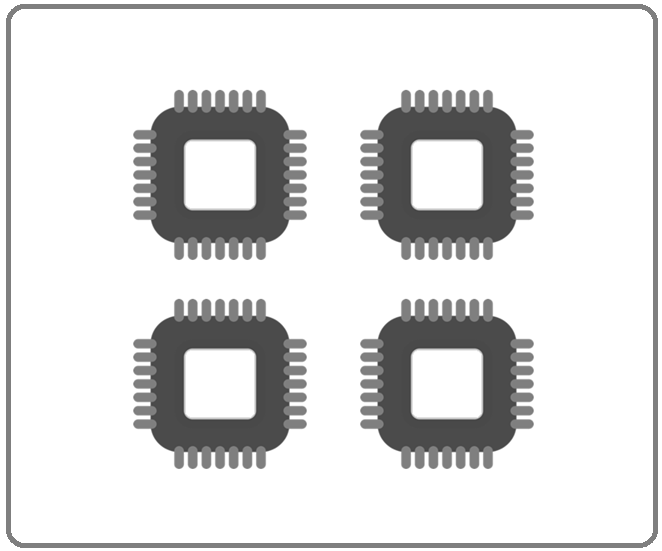
\includegraphics[width=10cm, height=9cm]{titlePicture}
        
        \vspace*{\fill}
        
        \begin{large}
            Санкт-Петербург \\ \the\year
        \end{large}
    \end{bfseries}   
\end{center}

% Старый вариант
% \thispagestyle{empty}
% \begin{center}
%     \begin{figure}
%         \centering
%         
\includegraphics[scale=0.15]{itmo_logo_black_2022}
%     \end{figure}
%     \textbf{\Large\centerline{В.В. Соснин, П.В. Балакшин, Д.С. Шилко,}} 
%     \textbf{\Large\centerline{Д.А. Пушкарев, А.В. Мишенёв,}} 
%     \textbf{\Large\centerline{П.В. Кустарев, А.А. Тропченко}}
    
%     \vspace*{\fill}
    
%     \Large\textbf{\centerline{ВВЕДЕНИЕ В ПАРАЛЛЕЛЬНЫЕ ВЫЧИСЛЕНИЯ}}
    
%     \vspace*{\fill}
    
%     \makebox[14cm]{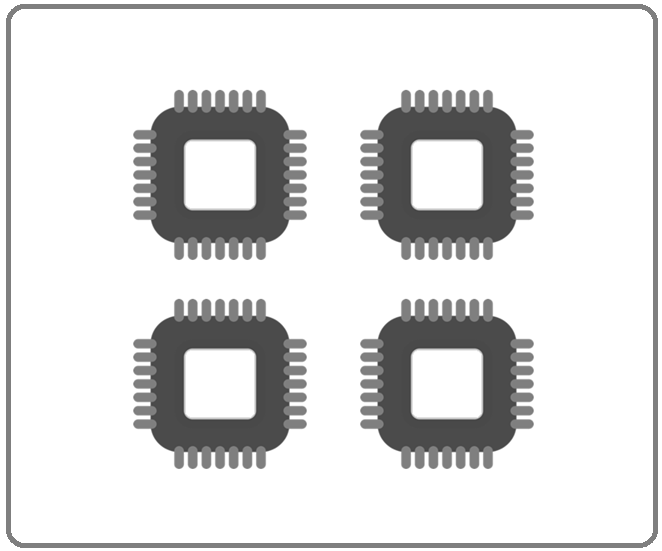
\includegraphics[width=10cm, height=9cm]{titlePicture}}
    
%     \vspace*{\fill}
    
%     \textbf{Санкт-Петербург}
    
%     \textbf{\the\year}
% \end{center}
% %сделать отступы между строками!!! %обложка, не идеёт в счёт страниц
	\thispagestyle{empty}

\begin{center}
    \noindent МИНИСТЕРСТВО НАУКИ И ВЫСШЕГО ОБРАЗОВАНИЯ РОССИЙСКОЙ ФЕДЕРАЦИИ
    \\[\baselineskip]
    УНИВЕРСИТЕТ ИТМО
    \\[2\baselineskip]
    \begin{bfseries}
        \begin{Large}
            В.В. Соснин, П.В. Балакшин, А.В. Мишенёв 
            \\[\baselineskip]
            \centerline{ВВЕДЕНИЕ В ПАРАЛЛЕЛЬНЫЕ ВЫЧИСЛЕНИЯ}
        \end{Large}
    \end{bfseries}
    
    \bigskip
    
    УЧЕБНО-МЕТОДИЧЕСКОЕ ПОСОБИЕ
    \\[\baselineskip]
    РЕКОМЕНДОВАНО К ИСПОЛЬЗОВАНИЮ В УНИВЕРСИТЕТЕ ИТМО
        
    по направлениям подготовки <<09.04.04 -- Программная инженерия>>, <<09.04.01 -- Информатика и вычислительная техника>> для реализации основных профессиональных образовательных программ магистратуры

    \vspace{\fill}

    
\includegraphics[scale=0.15]{itmo_logo_black_2022}

    \bigskip

    \begin{bfseries}
        \begin{large}
            Санкт-Петербург \\ 
            \the\year
        \end{large}
    \end{bfseries}
    
\end{center}

    \thispagestyle{empty}
 
Соснин В.В., Балакшин П.В., Мишенёв А.В. Введение в параллельные вычисления. -- СПб: Университет ИТМО, \the\year. -- \pageref{LastPage}~с. \\

Рецензент: Зилинберг А.Ю., к.т.н., доцент кафедры радиотехнических систем, ФГАОУ ВО <<Санкт-Петербургский государственный университет аэрокосмического приборостроения>>. \\

В пособии излагаются основные понятия и определения теории параллельных вычислений. Рассматриваются основные принципы построения программ на языке <<Си>> для многоядерных и многопроцессорных вычислительных комплексов с общей памятью. Предлагается набор заданий для проведения лабораторных и практических занятий. \\

Учебное пособие предназначено для студентов, обучающихся по магистерским программам направления <<09.04.04 -- Программная инженерия>>, <<09.04.01 -- Информатика и вычислительная техника>>, и может быть использовано выпускниками (бакалаврами и магистрантами) при написании выпускных квалификационных работ, связанных с проектированием и исследованием многоядерных и многопроцессорных вычислительных комплексов.
	%\parРекомендовано к печати Ученым советом факультета компьютерных технологий и управления, 8 декабря 2015 года, протокол №10.\textbf{НЕТ!!!!}

\vspace*{\fill}

\begin{flushright}
    
\includegraphics[scale=0.15]{itmo_logo_black_2022}
\end{flushright}

Университет ИТМО – ведущий вуз России в области информационных и фотонных технологий, один из немногих российских вузов, получивших в 2009 году статус национального исследовательского университета. С 2013 года Университет ИТМО -- участник программы повышения конкурентоспособности российских университетов среди ведущих мировых научно-образовательных центров, известной как проект <<5 в 100>>. Цель Университета ИТМО -- становление исследовательского университета мирового уровня, предпринимательского по типу, ориентированного на интернационализацию всех направлений деятельности.
\begin{flushright}
    \copyright\spaceУниверситет ИТМО, \the\year
    
    \copyright\spaceСоснин~В.В., Балакшин~П.В., Мишенёв~А.В., \the\year
\end{flushright}

    
    \setcounter{page}{3}
    \addtocontents{toc}{\protect\sloppy}
    \tableofcontents
    
	\phantomsection
\section*{Введение}
\addcontentsline{toc}{section}{Введение}

В настоящее время большинство выпускаемых микропроцессоров являются многоядерными. Это касается не только настольных компьютеров, но и в том числе мобильных телефонов и планшетов (исключением пока являются только встраиваемые вычислительные системы). Для полной реализации потенциала многоядерной системы программисту необходимо использовать специальные методы параллельного программирования, которые становятся всё более востребованными в промышленном программировании. Однако методы параллельного программирования ощутимо сложнее для освоения, чем традиционные методы написания последовательных программ~\cite{Galiakhmetova2019}.

Целью настоящего учебного пособия является описание практических заданий (лабораторных работ), которые можно использовать для закрепления теоретических знаний, полученных в рамках лекционного курса, посвященного технологиям параллельного программирования. Кроме этого, в пособии в сжатой форме излагаются основные принципы параллельного программирования.%, при этом теоретический материал даётся тезисно и поэтому для полноценного освоения требуется использовать конспекты лекций по соответствующей дисциплине.

При программировании многопоточных приложений приходится решать конфликты, возникающие при одновременном доступе к общей памяти нескольких потоков. Для синхронизации одновременного доступа к общей памяти в настоящее время используются следующие три концептуально различных подхода:

\begin{enumerate}
    \sloppy
    \item\textbf{Явное использование блокирующих примитивов} (мьютексы, семафоры, условные переменные). Этот подход исторически появился первым и сейчас является наиболее распространённым и поддерживаемым в большинстве языков программирования. Недостатком метода является достаточно высокий порог вхождения, т.к. от программиста требуется в <<ручном режиме>> управлять блокирующими примитивами, отслеживая конфликтные ситуации при доступе к общей памяти.
    \item\textbf{Применение программной транзакционной памяти} (Software Transactional Memory, STM). Этот метод проще в освоении и применении, чем предыдущий, однако до сих пор имеет ограниченную поддержку в компиляторах, а также в полной мере он сможет себя проявить при более широком распространении процессоров с аппаратной поддержкой STM\@.
    \item\textbf{Использование неблокирующих алгоритмов} (lockless, lock-free, wait-free algorithms). Этот метод подразумевает полный отказ от применения блокирующих примитивов при помощи сложных алгоритмических ухищрений. При этом для корректного функционирования неблокирующего алгоритма требуется, чтобы процессор поддерживал специальные атомарные (бесконфликтные) операции вида <<сравнить и обменять>> (cmpxchg, <<compare and swap>>). На данный момент большинство процессоров имеют в составе системы команд этот тип операций (за редким исключением, например: <<SPARC 32>>).
\end{enumerate}

Предлагаемое вниманию методическое пособие посвящено первому из перечисленных методов, т.к. он получил наибольшее освещение в литературе и наибольшее применение в промышленном программировании. Два других метода могут являться предметом изучения углублённых учебных курсов, посвященных параллельным вычислениям.

Авторы ставили целью предложить читателям изложение основных концепций параллельного программирования в сжатой форме в расчёте на самостоятельное изучение пособия в течение двух-трёх месяцев. При использовании пособия в технических вузах рекомендуется приведённый материал использовать в качестве односеместрового учебного курса в рамках %бакалаврской
подготовки студентов по направлению подготовки <<Программная инженерия>> или смежных с ней.% Однако приводимые примеры практических заданий могут быть при желании адаптированы для использования в магистерских курсах.

Данное пособие является дополненной и переработанной версией пособия авторов, выпущенного в 2015 году~\cite{SosninBalakshin2015}.
	\section{Теоретические основы параллельных вычислений}
\label{sec:parallel-theory}

\subsection{История развития параллельных вычислений}
\label{subsec:parallel-history}

Разговор о развитии параллельного программирования принято начинать истории развития суперкомпьютеров.
Однако первый в мире суперкомпьютер CDC6600, созданный в 1963 г., имел только один центральный процессор, поэтому едва ли можно считать его полноценной SMP-системой.
Архитектура SMP (от англ.\ Symmetric Multiprocessing) подразумевает работу несколько идентичных процессоров с общей для них оперативной памятью.
Многоядерный процессор можно считать частным случаем SMP-системы.

Третий в истории суперкомпьютер CDC8600 проектировался для использования четырёх процессоров с общей памятью, что позволяет говорить о первом случае применения SMP, однако CDC8600 так никогда и не был выпущен: его разработка была прекращена в 1972 году.

Лишь в 1983 году удалось создать работающий суперкомпьютер (Cray X-MP), в котором использовалось два центральных процессора, использовавших общую память.
Справедливости ради стоит отметить, что чуть раньше (в 1980 году) появился первый отечественный многопроцессорный компьютер Эльбрус-1, однако он по производительности значительно уступал суперкомпьютерам того времени.

Уже в 1994 можно был свободно купить настольный компьютер с двумя процессорами, когда компания ASUS выпустила свою первую материнскую плату с двумя сокетами, т.е. разъёмами для установки процессоров.

Следующей вехой в развитии SMP-систем стало появление многоядерных процессоров.
Первым многоядерным процессором массового использования стал POWER4, выпущенный фирмой IBM в 2001 году.
Но по-настоящему широкое распространение многоядерная архитектура получала лишь в 2005 году, когда компании AMD и Intel выпустили свои первые двухъядерные процессоры.

На рисунке~\ref{fig:GraphPartOfMultiCoreProcessorFromYear} показано, какую долю занимали процессоры с разным количеством ядер при создании суперкомпьютеров в разное время~\cite{Top500}. %(по материалам сайта \url{http://top500.org}).
Закрашенные области помечены цифрами для обозначения количества ядер.
Ширина области по вертикали равна относительной частоте использования процессоров соответствующего типа в рассматриваемом году.

\begin{figure}[H]
    \centering
    \includegraphics[width=0.95\linewidth]{GraphPartOfMultiCoreProcessorFromYear}
    \caption{Частотность использования процессоров с различным числом ядер при создании суперкомпьютеров}
    \label{fig:GraphPartOfMultiCoreProcessorFromYear}
\end{figure}

Как видим, активное использование двухъядерных процессоров в суперкомпьютерах началось уже в 2002 году, а примерно к 2005 году совершенно сошло на нет, тогда как в настольных компьютерах их применение в 2005 году лишь начиналось.
На основании этого можно сделать простой прогноз распространённости многоядерных <<настольных>> процессоров к нужному году, если считать, что они в общих чертах повторяют развитие многоядерных архитектур суперкомпьютеров.

\subsection{Термины и определения}
\label{subsec:terms-and-definitions}

Русскоязычная терминология в области параллельных вычислений (ПВ) не всегда однозначно соответствует англоязычной, поэтому ниже для каждого термина даётся его англоязычный вариант и делается поправка на неидентичность этих терминов, где это необходимо.  

\textbf{Параллельные вычисления (concurrent computing)} -- способ организации вычислений на одном или нескольких компьютерах, при котором пересекаются периоды жизни нескольких задач.
Антонимом этого термина являются {\bfseries последовательные вычисления (sequential computing)}, при выполнении которых периоды жизни задач не пересекаются.
Например, пусть $start_i$, $end_i$ - это соответственно времена начала и конца жизни вычислительной задачи $i$, и пусть ${start_1 < start_2}$, тогда:

\begin{itemize}
    \item при $end_1 < start_2$ имеют место последовательные вычисления;
    \item при $end_1 \ge start_2$ имеют место параллельные вычисления.
\end{itemize}

Англоязычный термин \textbf{parallel computing} переводится на русский язык тем же словосочетанием: параллельные вычисления.
% TODO: Запятая после однако?
Однако в него вкладывается более узкий, чем в concurrent computing, смысл: при parallel computing задачи исполняются физически одновременно на различных процессорах и/или ядрах одного компьютера.
Это значит, что понятие concurrent включает в себя parallel, а именно: любые parallel-вычисления являются concurrent, но не всякие concurrent-вычисления являются parallel.

Классический пример concurrent-вычислений, которые не являются parallel, -- это реализация многозадачности в операционной системе (ОС) при наличии только одного одноядерного процессора.
В этом случае ОС не может физически параллельно выполнять разные задачи и вынуждена запускать их в режиме разделения времени, т.е. поочерёдно разрешая использовать процессор разным задачам, переключаясь с задачи на задачу по несколько раз до окончания выполнения каждой из них.

Иногда parallel computing переводится как \textbf{многоядерные вычисления (multicore computing)}, чтобы подчеркнуть отличие от con\-current computing, однако этот термин неидеален, т.к. не позволяет корректно классифицировать вычисления на многопроцессорных компьютерах, в которых каждый процессор является одноядерным.
Такие компьютеры позволяют выполнять parallel computing, но не multicore computing.
Но этой проблемой можно пренебречь, т.к. подобных компьютеров в данный момент практически нет на рынке.
Более точным термином можно считать SMP (shared memory processing), который относится к работе параллельных программ на системах с общей памятью.
В таких системах все процессоры/ядра совместно используют общую оперативную память одного компьютера.
Итак, можно установить следующие пары соответствий:

\begin{itemize}
    \item параллельные вычисления $\neq$ parallel computing;			
    \item параллельные вычисления $=$ concurrent computing;
    \item многоядерные вычисления $=$ parallel computing;
    \item parallel computing $=$ multicore computing $=$ SMP\@.
\end{itemize}

\textbf{Распределённые вычисления (distributed computing)} -- такие ПВ, при которых для решения задачи вычисления происходят на процессорах, расположенных на разных компьютерах, соединённых сетью, т.е. для выполнения вычислений приходится передавать программы и/или данные по сети.

Классификация ПВ по особенностям аппаратной реализации:

\begin{enumerate}
    \sloppy
    \item\textbf{Параллелизм на уровне битов} -- процессор выполняет операцию для всех битов машинного слова одновременно.
    Например, 64-разрядный процессор может одновременно инвертировать значение каждого из 64 битов заданного операнда.
    \item\textbf{Параллелизм на уровне операндов} -- одна инструкция процессора позволяет выполнить некоторую операцию для целого массива операндов параллельно.
    Например, с помощью технологии SSE за одну операцию можно попарно перемножить элементы двух массивов.\ (все умножения будут выполнены параллельно во времени).
    \item\textbf{Параллелизм на уровне инструкций} -- выполнение каждой инструкции разбивается на фазы, каждая из которых может выполняться процессором физически параллельно.
    Это изменение архитектуры процессора никак не влияет на общее время выполнения одной изолированной инструкции, однако при обработке нескольких подряд идущих инструкций удаётся организовать из них конвейер.
    В результате подряд идущие инструкции выполняются физически параллельно, что позволяет увеличить общую производительность процессора, выраженную в инструкциях/с (см.\ детали ниже в этом разделе).
\end{enumerate}

%\par\sout{Важно различать понятия ''параллельные вычисления'' и ''параллельные технологии''. Разберем следующие понятия, которые, хотя и являются параллельными технологиями (на уровне ядра или межъядерного взаимодействия), однако не являются параллельными вычислениями, но часто \textbf{по ошибке} причисляются к ним}:

Перечисленные далее параллельные технологии в данном пособии рассматриваются кратко, чуть шире, чем определения.

\begin{itemize}
    \sloppy
    \item\textit{Конвейерная обработка данных (суперскалярность)} представляет собой одновременную обработку процессором нескольких инструкций, при котором в один момент времени для каждой из инструкций выполняется различный этап выполнения.
    Например, если какой-либо процессор может одновременно получать, раскодировать и выполнить инструкцию, то он во время получения первой инструкции может раскодировать вторую и выполнять третью (рисунок~\ref{fig:simd_pipeline}). Этот способ организации вычислений не является параллельными вычислениями, потому что инструкции все равно выполняются последовательно, а задействовано только одно ядро.
    
    \begin{figure}[H]
         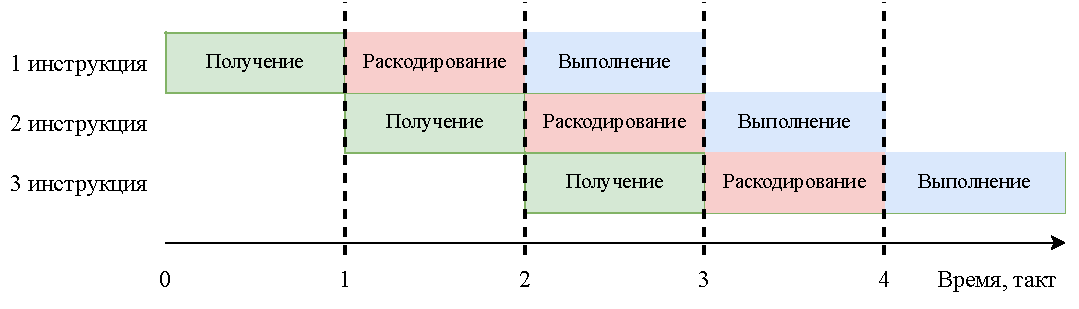
\includegraphics[width=\linewidth]{simd-pipeline}
         \caption{\textit{Конвейерная обработка инструкций}}
         \label{fig:simd_pipeline}
    \end{figure}
    
    \item\textit{SIMD-расширения (MMX, SSE)} обеспечивают параллелизм на уровне данных.
    Например, процессор может одновременно умножать четыре числа вместо одного с помощью SSE инструкции.
%    TODO: Запятая после однако?
    Однако поток команд все равно остается одиночным, т.е. выполняется одна инструкция программы за промежуток времени, что не является случаем параллельных вычислений.
    \item\textit{Вытесняющая многозадачность} организуется операционной системой.
    Несколько процессов стоят в очереди выполнения и ОС сама решает как распорядиться процессорным временем между ними.
    Если у первого потока задан больший приоритет, чем у второго, то ОС будет выделять больше времени на выполнение первого потока, однако в один момент времени будет выполняться только один поток, следовательно, вытесняющая многозадачность тоже не входит в понятие параллельных вычислений.
\end{itemize}

Для организации параллельных вычислений используются различные технологии распараллеливания:

\begin{itemize}
    \item\textbf{Process (процесс)} -- наиболее тяжеловесный механизм, применяемый для распараллеливания.
    Каждый процесс имеет свое независимое адресное пространство, поэтому синхронизация данных между процессами долгая и сложная.
    Может включать в себя несколько потоков исполнения.
    \item\textbf{Thread (поток исполнения, нить, тред, поток)} выполняется независимо от других потоков, но имеет общее адресное пространство с другими потоками в рамках одного процесса.
    На этом уровне используется механизмы синхронизации данных (будут рассмотрены далее).
    \item\textbf{Fiber (волокно)} -- легковесный поток выполнения.
    Также как и треды, fiber'ы имеют общее адресное пространство, однако используют совместную многозадачность вместо вытесняющей.
    ОС не переключает контекст из одного треда в другой, вместо этого главный поток сам выделяет время для работы дочернего fiber, либо блокируется логически (то есть жизненным циклом fiber'a управляет программист).
    Также все fiber'ы работают на одном ядре, в отличие от тредов, которые могут работать на разных ядрах.
\end{itemize}

Для лучшего понимания тредов схематично рассмотрим его жизненный цикл (lifecycle).
На рисунке~\ref{fig:thread-lifesycle} видно, что поток может находиться в трех состояниях -- готовность, ожидание и выполнение.
После создания потока он пребывает в состоянии готовности.
Затем ОС принимает решение о смене его состояния (вытесняющая многозадачность).
Для fiber жизненный цикл такой же, но переходами между ними управляет программист или механизмы синхронизации.

Разные стандарты языков программирования могут добавлять в жизненный цикл потоков новые состояния, например, блокировка потока, прерывание работы потока и остальные, однако общая схема работы остается той же.

\begin{figure}[H]
    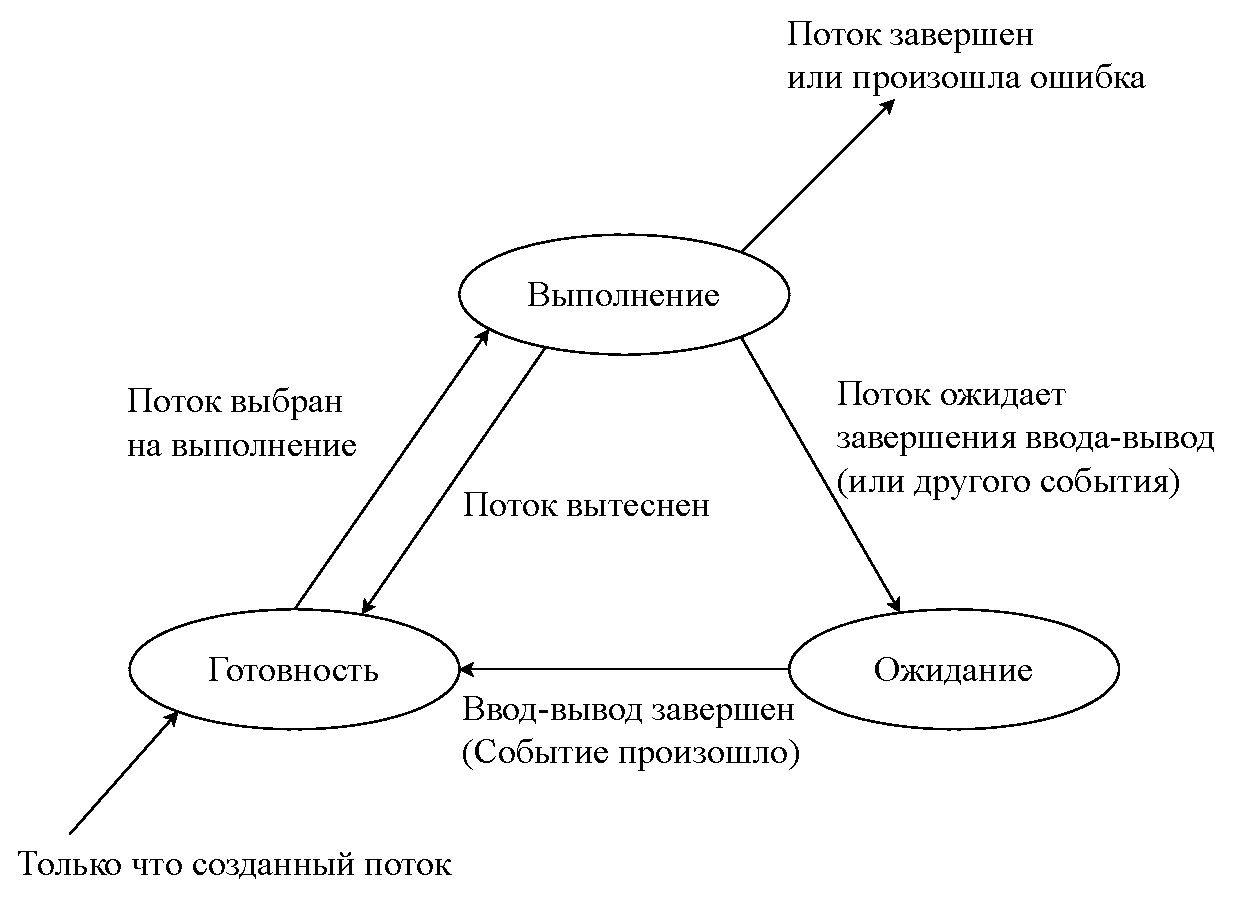
\includegraphics[width=\linewidth]{thread_lifecycle}
    \caption{Жизненный цикл потока}
    \label{fig:thread-lifesycle}
\end{figure}

\sloppy
В среде программистов существуют понятия \textbf{потокобезопасной (thread-safe)} и \textbf{реентерабельной (reentrant или reenterable)} функции, однако в разных сообществах они могут иметь различные значения.
В таблице~\ref{tab:thread_safe_reentrant} написаны определения из разных источников.

\begin{table}[H]
    \caption{Определения thread-safe и reentrant функций}
    \label{tab:thread_safe_reentrant}
    \begin{tabularx}{\textwidth}{|c|C|C|}
        \hline
        \thead{Источник \\ определения} & \thead{Thread-safe} & \thead{Reentrant} \\ \hline
        QT & Внутри функции обращение ко всем общим переменным осуществляется строго последовательно, а не параллельно (Thread-safe является reentrant, но не наоборот) & При вызове функции одновременно несколькими потоками гарантируется правильная работа, только если потоки не используют общие данные \\ \hline
        Linux & Функция показывает правильные результаты, даже если вызвана несколькими тредами одновременно & Функция показывает правильные результаты, даже если повторно вызвана изнутри себя \\ \hline
        POSIX &  & Функция показывает правильные результаты, даже если вызвана несколькими тредами одновременно \\ \hline
    \end{tabularx}
\end{table}

Рассмотрим примеры функций, подходящие под определение сообщества Linux.
\inputminted{c++}{listings/swapExample1.cpp}

Данная функция не является ни потокобезопасной, ни реентерабельной, потому что все потоки, вызывающие ее, будут использовать общую переменную t.
Если вызвать функцию внутри ее самой, то перезапишется значение t и родительская функция отработает неправильно.
Попробуем исправить эти ошибки, объявив переменную t типа \_\_thread int.

\inputminted{c++}{listings/swapExample2.cpp}

Теперь компилятор создаст копию переменной для каждого потока t, и функция станет потокобезопасной, однако она все еще не реентерабельной по той же причине.
Будем сохранять значение глобальной переменной t в начале функции и восстанавливать ее в конце.

\inputminted{c++}{listings/swapExample3.cpp}

Новая функция реентерабельна, но снова потоконебезопасна.
Наконец, приведем пример реализации swap(), которая потокобезопасна и реентерабельна:

\inputminted{c++}{listings/swapExample4.cpp}

\subsection{Классификация параллельных систем (архитектур)}
\label{subsec:architecture-classification}

По физической архитектуре параллельные системы можно разделить на два типа:

\begin{enumerate}
    \item\textbf{SMP} (Shared Memory Parallelism, Symmetric MultiProcessor system) -- многопроцессорность, многоядерность, GPGPU\@. 
    \item\textbf{MPP} (Massively Parallel Processing) -- кластерные системы, GRID (распределенные вычисления).
\end{enumerate}

Далее рассмотрим эти две архитектуры подробнее.

\textbf{\textit{SMP}} -- архитектура многопроцессорных систем, в которой два или более одинаковых процессора сравнимой производительности подключаются единообразно к общей памяти (и периферийным устройствам) и выполняют одни и те же функции (почему, собственно, система и называется симметричной).
В английском языке SMP-системы носят также название tightly coupled multiprocessors, так как в этом классе систем процессоры тесно связаны друг с другом через общую шину, имеют равный доступ ко всем ресурсам вычислительной системы (памяти и устройствам ввода-вывода) и управляются лишь одним экземпляром операционной системы~\cite{SymmetricMultiprocessingWP}.
В этой архитектуре все процессоры расположены на одной физической машине, поэтому они имеют общие банки памяти.
Существует два вида подключения процессоров к общей памяти.

\textit{Соединение по общей шине (system bus)} изображено на рисунке~\ref{fig:smp_system_bus}.
В этом случае только один процессор может обращаться к памяти в каждый данный момент, что накладывает существенное ограничение на количество процессоров, поддерживаемых в таких системах.
Чем больше процессоров, тем больше нагрузка на общую шину, тем дольше должен ждать каждый процессор, пока освободится шина, чтобы обратиться к памяти.
Снижение общей производительности такой системы с ростом количества процессоров происходит очень быстро, поэтому обычно в таких системах количество процессоров не превышает 2--4.
Примером SMP-машин с таким способом соединения процессоров являются любые многопроцессорные серверы начального уровня~\cite{Martyshkin2014}.

\begin{figure}[H]
    \centering
    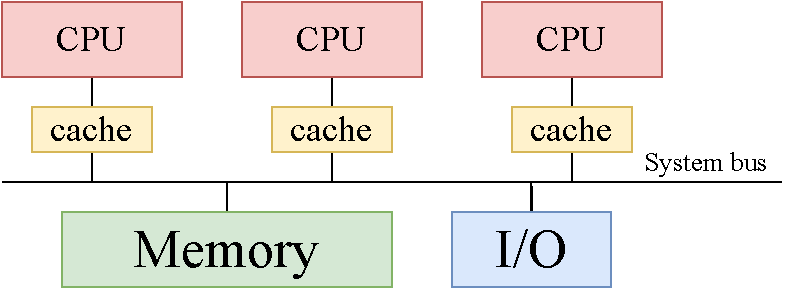
\includegraphics[width=0.9\linewidth]{smp_system_bus}
    \caption{Архитектура SMP. Подключение процессоров по системной шине}
    \label{fig:smp_system_bus}
\end{figure}

\textit{Коммутируемое соединение (crossbar switch)} изображено на рисунке~\ref{fig:smp-crossbar-switch}.
При таком соединении вся общая память делится на банки памяти, каждый банк памяти имеет свою собственную шину, и процессоры соединены со всеми шинами, имея доступ по ним к любому из банков памяти.
Такое соединение схемотехнически более сложное, но оно позволяет процессорам обращаться к общей памяти одновременно.
Это позволяет увеличить количество процессоров в системе до 8--16 без заметного снижения общей производительности~\cite{Ryazanova2018}.

Плюсами такого подхода является высокая скорость обмена данными между процессорами и относительная простота в разработке ПО.
Однако могут возникнуть проблемы с масштабируемостью системы (если на материнской плате есть только два сокета, то три процессора уже не поставить).

\begin{figure}[H]
    \centering
    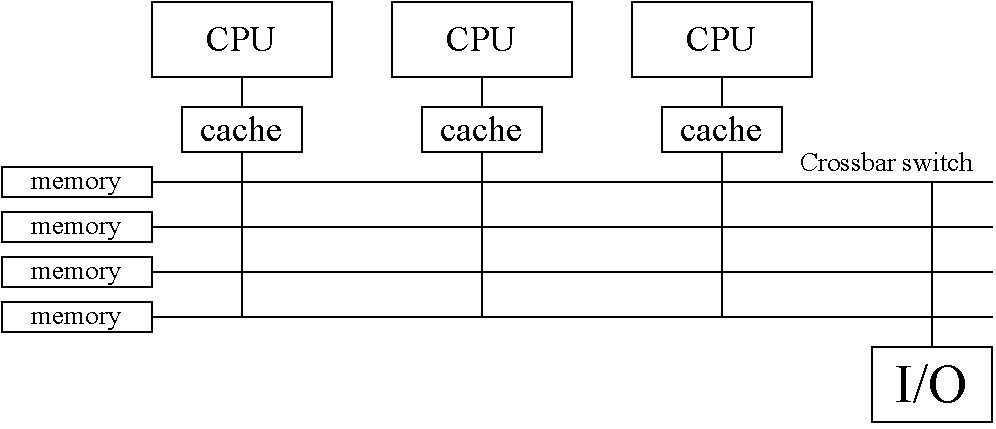
\includegraphics[width=\linewidth]{smp_crossbar_switch}
    \caption{Архитектура SMP. Подключение процессоров через коммутируемое соединение}
    \label{fig:smp-crossbar-switch}
\end{figure}

\textbf{\textit{MMP}} -- архитектура многопроцессорных систем, при которой память между процессорами разделена физически.
На таких системах проводятся распределенные вычисления.
Система строится из отдельных узлов, содержащих процессор, локальный банк оперативной памяти, коммуникационные процессоры или сетевые адаптеры, иногда - жёсткие диски и другие устройства ввода-вывода.
Доступ к банку оперативной памяти данного узла имеют только процессоры из этого же узла.
Узлы соединяются специальными коммуникационными каналами (рисунок~\ref{fig:mmp}).

\begin{figure}[H]
    \centering
    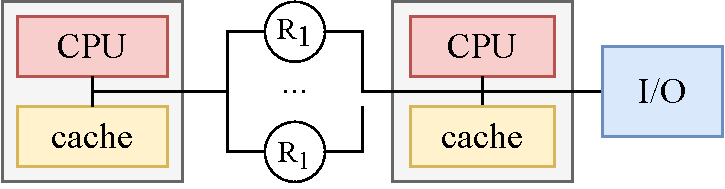
\includegraphics[width=0.9\linewidth]{mmp}
    \caption{Архитектура MMP}
    \label{fig:mmp}
\end{figure}

Плюсами такого подхода является хорошая масштабируемость (при необходимости в увеличении производительности системы достаточно просто добавить еще узлов).
Однако существенно понижается скорость межпроцессорного обмена, так как теперь банки памяти разнесены физически.
Также стоимость ПО, распределяющее вычисления, очень высока.

\subsection{Методы синхронизации в параллельных программах}
\label{subsec:syncronization-methods}

В параллельных программах разработчик часто сталкивается с проблемой синхронизации между потоками.
Как правило, проблемы возникают при доступе к памяти и одновременном выполнении каких-то критических участков кода --- критических секций.

\textbf{Критической областью} называют секцию программы, которая должна выполняться с исключительным правом доступа к разделяемым данным, на которые имеются ссылки в этой программе.
Процесс, готовящийся войти в критическую область, может быть задержан, если любой другой процесс в это время выполняется в подобной критической области.

В этом разделе будут подробно рассмотрены механизмы синхронизации потоков на программном уровне.

Существуют следующие методы решения проблем синхронизации потоков:
\begin{itemize}
    \item\textbf{Атомарные операции} -- операции, которые выполняются целиком или не выполняются вовсе.
    Например, транзакция к БД является атомарной операцией.
    Когда два потока пытаются инкрементировать одну и ту же ячейку памяти несинхронизированно, значение может увеличиться на два, а может и на один в зависимости от поведения потоков, так как операция инкрементации представляет собой как минимум три ассемблерные инструкции.
    Чтобы избежать этого, стоит объявлять тип данных атомарным (если таковой есть в данном языке программирования/библиотеке).
    Частным случаем атомарных операций являются read-modify-write операции: compare-and-swap, test-and-set, fetch-and-add.
    Подробнее проблема реализации атомарных операций будет поднята в разделе~\ref{subsec:atomic-operations} \textit{Атомарность операций в многопоточной программе}.
    
    \item\textbf{Семафор} -- объект, ограничивающий число потоков, которые могут войти в эту область кода.
    Как правило, это число задается при инициализации семафора.
    Затем при захвате семафора новым потоком проверяется количество потоков, уже захвативших семафор.
    Если максимальное число потоков достигнуто, то новый поток будет ждать, пока какой-то из потоков, вошедших в область кода, освободит его.
    Часто использование семафоров неоправданно, так как накладные расходы на создание и поддержку семафора большие.
    Также следует избегать <<утечки семафора>>, ситуации, при которой поток не выходит из семафора при окончании выполнения области кода, если программист забыл освободить ресурс.
    
    \item\textbf{Reader/writer semaphore} предоставляет потокам права \textit{только} на чтение или запись, причем во время записи данных одним потоком остальные потоки не имеет доступа к ресурсу.
    Однако в таких семафорах может быть проблема \textit{ресурсного голодания (starvation)}, при котором, пока потоки будут читать данные, другие потоки не смогут записать данные долгий промежуток времени или наоборот.
    Частным решением этой проблемы при равном приоритете потоков может быть поочередный доступ потоков в очереди к чтению и записи.
    
    \item{\textbf{Мьютекс} -- частный случай семафора, при котором данную область кода может захватывать только один поток. В случае, если мьютекс обслуживает несколько критических секций, только один поток может находиться в любой из критических секций. Часто используется при организации управления критическими секциями, так как <<легче>> классического семафора (достаточно хранить одну булеву переменную вместо счетчика), но в отличии от него, предполагается, что один и тот же поток будет захватывать и освобождать мьютекс. Следует отметить, что в стандарте языка C++11, кроме стандартного мьютекса, существуют разные его модификации:  \textit{recursive\_mutex} -- мьютекс, допускающий повторный вход в критическую секцию этим же потоком, 
    \textit{timed\_mutex} -- мьютекс с таймером захвата и  \textit{recursive\_timed\_mutex}, совмещающий достоинства обеих версий.}
    
    \item\textbf{Spinlock (циклическая блокировка)} -- блокировка, при которой поток в цикле ожидает освобождения ресурса.
    Не всегда является оптимальным решением, так как ожидающий поток работает во время ожидания.
    Внутри секции кода необходимо избегать прерываний исполнения потока, чтобы избежать deadlock'a.
    
    \item\textbf{Seqlock (последовательная блокировка)} -- механизм синхронизации, предназначенный для быстрой записи переменной несколькими потоками.
    В ядре Linux работает следующим образом: поток ждет, пока критическая секция освободится(spinlock); при входе в секцию инкрементируется счетчик, поток делает свою работу.
    При выходе из секции поток проверяет значение счетчика.
    Если значение счетчика не изменилось, значит, в данный момент никто не записывал данные, и поток выходит из критической секции, иначе он считывает значение переменной заново.
    
    \item\textbf{Knuth–Bendix completion algorithm} -- одним из решений проблем синхронизации является алгоритм Кнута-Бендикса.
    С его помощью можно перейти от последовательной программы к каскадной.
    Однако не для всех программ этот алгоритм работает, иногда он может уйти в бесконечный цикл или завершиться с ошибкой.
    
    \item\textbf{Barrier (барьер)} в OpenMP -- участок кода, в котором синхронизируется состояние потоков (не путать с барьером памяти).
    Например, если для функции в главном потоке требуется, чтобы все дочерние потоки закончили свою работу, можно поставить барьер перед ней.
    Тогда она будет ждать завершения работы дочерних потоков, после чего все потоки продолжат свою работу.
    Примером реализации барьера может быть критическая секция, код которой разрешается выполняться только последнему потоку, запросившему выполнение.
    Остальные потоки должны ожидать его.
    Для этого необходимо знать, сколько потоков должно прийти в барьер.
    
    \item\textbf{Неблокирующие алгоритмы.} Часто бывает полезно не использовать стандартные приемы блокировки, а сделать алгоритм неблокирующим.
    В таком случае программист должен самостоятельно гарантировать, что критические секции кода не будут выполняться одновременно и целостность разделяемой памяти.
    Также плюсом таких алгоритмов является безопасная обработка прерываний.
    Для реализации таких алгоритмов часто используются другие технологии синхронизации: read-modify-write, CAS (см.\ раздел~\ref{subsec:atomic-operations}) и другие.
    
    \item\textbf{RCU (read-copy-update)} -- алгоритм, позволяющий потокам эффективно считывать данные, оставляя обновление данных на конец работы алгоритма, гарантируя при этом релевантные данные.
    Только один поток может писать данные, но читать данные могут сразу несколько потоков.
    Достигается это, например, путем атомарной подмены указателя (CAS). Старые версии данных хранятся для прошлых обращений, пока на них есть хотя бы один указатель.
    Существуют более новые инструменты для замены указателя: отдельная взаимная блокировка для писателей или механизм membarrier, использующийся в последних версия Linux.
    RCU может быть полезен при организации структур данных без явных блокировок.
    
    \item\textbf{Монитор} -- объект, инкапсулирующий в себе мьютекс и служебные переменные для обеспечение безопасного доступа к методу или переменной несколькими потоками.
    Характеризует монитор то, что в один момент только один поток может выполнять любой из его методов.
    Например, если у нас существует класс (в терминах C++) Account имеющий методы add\_money(), sub\_money(), то имеет смысл сделать его монитором, чтобы не было конфликтов при проведении операций с аккаунтом.
\end{itemize}

Однако необязательно организовывать параллельные вычисления, используя синхронизации или блокировки.
Некоторые технологии предлагают альтернативный подход к параллельным вычислениям:

\begin{itemize}
    \item\textbf{Программная транзакционная память} -- модель памяти, в которой операции, производимые над ячейками памяти атомарны.
    Плюсы использования: простота использования (заключения блоков кода в блок транзакции), отсутствие блокировок, однако при неправильном использовании возможно падение производительности, а также невозможность использования операций, которые нельзя отменить внутри блока транзакции.
    В компиляторе GCC поддерживается с версии 4.7 следующим образом:
    \begin{enumerate}
        \item\texttt{\_\_transaction\_atomic \{...\}} -- указание, что блок кода - транзакция;
        \item\texttt{\_\_transaction\_relaxed \{...\}} -- указание, что небезопасный код внутри блока не приводит к побочным эффектам \textit{(не поддерживается в версиях 9.x и выше)};
        \item\texttt{\_\_transaction\_cancel} -- явная отмена транзакции;
        \item\texttt{attribute((transaction\_safe))} -- указание тран\-зак\-ци\-он\-но-бе\-зо\-пас\-ной функции;
        \item\texttt{attribute((transaction\_pure))} -- указание функции без побочных эффектов.
    \end{enumerate}

    \item\textbf{Модель акторов} -- математическая модель параллельных вычислений, в которой программа представляет собой набор объектов-акторов, которые взаимодействуют между собой и могут создавать новых акторов, отправлять и посылать сообщения друг другу.
    Предполагается параллелизм вычислений внутри одного актора.
    Каждый актор имеет адрес, на который можно отправить сообщение.
    Каждый актор работает в отдельном потоке.
    Модель акторов используется для организации электронной почты, некоторых веб-сервисов SOAP и тд.
\end{itemize}

Несмотря на большое число методов синхронизации, чаще всего надо исходить из решаемой задачи.
Например, если мы хотим сделать общую инкрементируемую целочисленную переменную для нескольких потоков, нет смысла создавать mutex или semaphore, более оптимально сделать переменную атомарной.
Всегда надо учитывать накладные расходы на создание блокировок и время разработки.

\subsection{Автоматическое распараллеливание программ}
\label{subsec:automatic-parallelizaion}

Параллельное программирование – достаточно сложный ручной процесс, поэтому кажется очевидной необходимость его автоматизировать с помощью компилятора.
Такие попытки делаются, однако эффективность автораспараллеливания пока что оставляет желать лучшего, т.к. хорошие показатели параллельного ускорения достигаются лишь для ограниченного набора простых for-циклов, в которых отсутствуют зависимости по данным между итерациями и при этом количество итераций не может измениться после начала цикла.
Но даже если два указанных условия в некотором for-цикле выполняются, но он имеет сложную неочевидную структуру, то его распараллеливание производиться не будет.
Виды автоматического распараллеливания:

\begin{itemize}
    \item\textit{Полностью автоматический:} участие программиста не требуется, все действия выполняет компилятор.
    \item\textit{Полуавтоматический:} программист даёт указания компилятору в виде специальных ключей, которые позволяют регулировать некоторые аспекты распараллеливания.
\end{itemize}


Слабые стороны автоматического распараллеливания:

\begin{itemize}
    \itemВозможно ошибочное изменение логики программы.
    \itemВозможно понижение скорости вместо повышения.
    \itemОтсутствие гибкости ручного распараллеливания.
    \itemЭффективно распараллеливаются только циклы.
    \itemНевозможность распараллелить программы со сложным алгоритмом работы.
\end{itemize}

Приведём примеры того, как с-программа в файле src.c может быть автоматически распараллелена при использовании некоторых популярных компиляторов:

\begin{itemize}
    \itemКомпилятор GNU Compiler Collection:	 
    \mint[breaklines]{text}{gcc -O3 -floop-parallelize-all -ftree-parallelize-loops=K -fdump-tree-parloops-details src.c} 
    При этом программисту даётся возможность выбрать значение параметра K, который рекомендуется устанавливать равным количеству ядер (процессоров).
    Особенностям реализации автораспараллеливания в gcc посвящён самостоятельный проект~\cite{AutoParInGCC}.
    % : \url{https://gcc.gnu.org/wiki/AutoParInGCC}. 
    \itemКомпилятор фирмы Intel:
    \mint[breaklines]{text}{icc -c -parallel -par-report file.cc}
    \itemКомпилятор фирмы Oracle:
    \mint[breaklines]{text}{solarisstudio -cc -O3 -xautopar -xloopinfo src.c}
\end{itemize}

\subsection{Основные подходы к распараллеливанию}
\label{subsec:parallelization-approaches}

На практике сложилось достаточное большое количество шаблонов параллельного программирования.
Однако все эти шаблоны в своей основе используют три базовых подхода к распараллеливанию:

\begin{itemize}
    \item\textbf{Распараллеливание по данным:} Программист находит в программе массив данных, элементы которого программа последовательно обрабатывает в некоторой функции func.
    Затем программист пытается разбить этот массив данных на блоки, которые могут быть обработаны в func независимо друг от друга.
    Затем программист запускает сразу несколько потоков, каждый из которых выполняет func, но при этом обрабатывает в этой функции отличные от других потоков блоки данных.
    \item\textbf{Распараллеливание по инструкциям:} Программист находит в программе последовательно вызываемые функции, процесс работы которых не влияет друг на друга (такие функции не изменяют общие глобальные переменные, а результаты одной не используются в работе другой).
    Затем эти функции программист запускает в параллельных потоках.
    \item\textbf{Распараллеливание по информационным потокам:} Программа представляет собой набор выполняемых функций, причем несколько функций могут ожидать результата выполнения предыдущих.
    В таком случае каждое ядро выполняет ту функцию, данные для которой уже готовы.
    Рассмотрим этот метод на примере абстрактного двухъядерного процессора как наиболее сложный для понимания.
    Структурный алгоритм, изображенный на рисунке~\ref{fig:2-core-algorithm}, состоит из 9 функций, некоторые из которых используют результат предыдущей функции в своей работе.
    Будем считать, что функция 3 использует результат работы функции 1, а функция 7 - результат функций 4 и 6 и т.д., а также функция 5 выполняется по времени примерно столько же, сколько функции 7, 8 и 9, вместе взятые.
    Тогда на двухъядерной машине этот способ распараллеливания будет оптимальным решением.
\end{itemize}

\begin{figure}[H]
    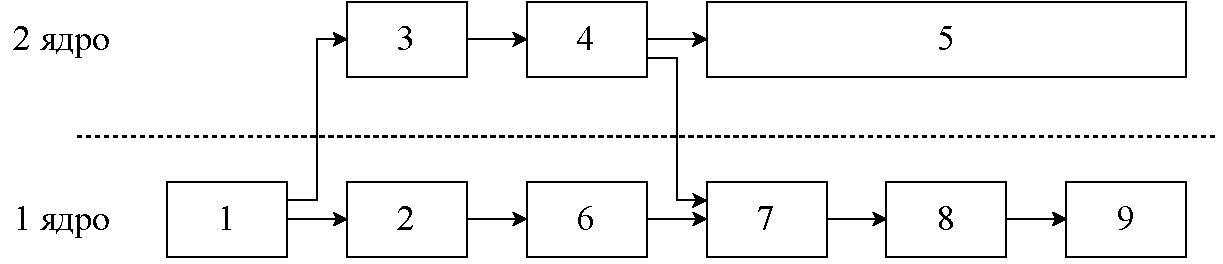
\includegraphics[width=\linewidth]{2-core_algorithm}
    \caption{Пример работы структурного алгоритма на двухъядерном процессоре}
    \label{fig:2-core-algorithm}
\end{figure}

% На практике сложилось достаточное большое количество шаблонов параллельного программирования. Однако все эти шаблоны в своей основе используют три базовых подхода к распараллеливанию: по данным, по инструкциям и по информационным потокам.

% \subsubsection*{Распараллеливание по данным}
% Программист находит в программе массив данных, элементы которого программа последовательно обрабатывает в некоторой функции func. Затем программист пытается разбить этот массив данных на блоки, которые могут быть обработаны в func независимо друг от друга. Затем программист запускает сразу несколько потоков, каждый из которых выполняет func, но при этом обрабатывает в этой функции отличные от других потоков блоки данных.

% \subsubsection*{Распараллеливание по инструкциям}
% Программист находит в программе последовательно вызываемые функции, процесс работы которых не влияет друг на друга (такие функции не изменяют общие глобальные переменные, а результаты одной не используются в работе другой). Затем эти функции программист запускает в параллельных потоках.

% \subsubsection*{Распараллеливание по информационным потокам}
% Программа представляет собой набор выполняемых функций, причем несколько функций могут ожидать результата выполнения предыдущих. В таком случае каждое ядро выполняет ту функцию, данные для которой уже готовы. Рассмотрим этот метод на примере абстрактного двухъядерного процессора, как наиболее сложный для понимания. Структурный алгоритм, изображенный на рисунке~\ref{structAlgorithm:image} состоит из 9 функций, некоторые из которых используют результат предыдущей функции в своей работе. Будем считать, что функция 3 использует результат работы функции 1, а функция 7 -- результат функций 4 и 6 и т.д., а также функция 5 выполняется по времени примерно столько же сколько функции 7, 8 и 9, вместе взятые. Тогда, на двухъядерной машине этот способ распараллеливания будет оптимальным решением.

% \begin{figure}[H]
%     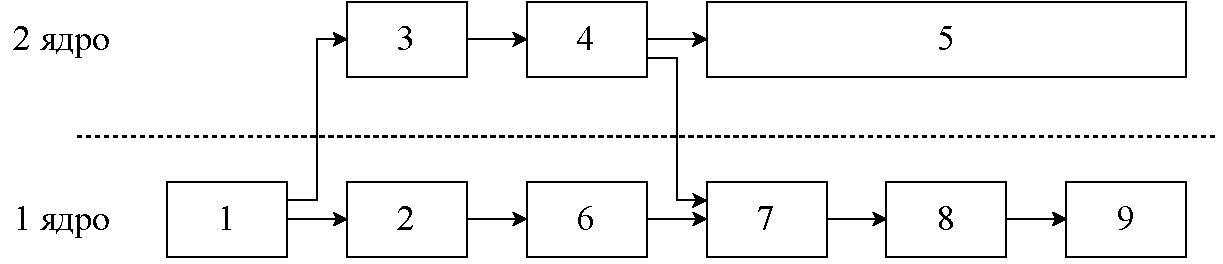
\includegraphics[width=\linewidth]{2-core_algorithm}
%     \caption{Пример работы структурного алгоритма на двухъядерном процессоре}
%     \label{structAlgorithm:image}
% \end{figure}

Три описанных метода легче понять на аналогии из обыденной жизни.
Пусть два студента получили в стройотряде задание подмести улицу и покрасить забор.
Если студенты решат использовать распараллеливание по данным, он будут сначала вместе подметать улицу, а затем вместе же красить забор.
Если они решат использовать распараллеливание по инструкциям, то один студент полностью подметёт улицу, а другой покрасит в это время весь забор.
Распараллелить по информационным потокам эту ситуацию не получится, так как эти два действия никак не зависят друг от друга.
Если предположить, что им обоим нужны инструменты для работы, то один из них должен сначала сходить за ними, а потом они оба начнут делать свою работу.

В большем числе случаев решение об использовании метода является очевидным в силу внутренних особенностей распараллеливаемой программы.
Выбор метода определяется тем, какой из них более равномерно загружает потоки.
В идеале все потоки должны приблизительно одновременно заканчивать выделенную им работу, чтобы оптимально загрузить ядра (процессоры) и чтобы закончившие работу потоки не простаивали в ожидании завершения работы соседними потоками.

\subsection{Атомарность операций в многопоточной программе}
\label{subsec:atomic-operations}

Основной проблемой при параллельном программировании является необходимость устранять конфликты при одновременном доступе к общей памяти нескольких потоков.
Для решения этой проблемы обычно пытаются упорядочить доступ потоков к общим данным с помощью специальных средств – примитивов синхронизации.
Однако возникает вопрос, существуют ли такие элементарные атомарные операции, выполнение которых несколькими потоками одновременно не требует синхронизации действий, т.к. эти операции выполнялись бы процессором <<одним махом>>, или – как принято говорить – <<атомарно>> (т.е. никакая другая операция не может вытеснить из процессора предыдущую атомарную операцию до её окончания).

Такими операциями являются практически все ассемблерные инструкции, т.к. они на низком уровне используют только те операции, которые присутствуют в системе команд процессора, а значит могут выполняться атомарно (непрерываемо).
Однако при компиляции С программы команды языка С транслируются обычно в несколько ассемблерных инструкций.
В связи с этим возникает вопрос о возможном существовании С-команд, которые компилируются в одну ассемблерную инструкцию.
Такие команды можно было бы не <<защищать>> примитивами синхронизации (мьютексами) при параллельном программировании.

Однако оказывается, что таких операций крайне мало, а некоторые из них могут вести себя как атомарно, так и неатомарно в зависимости от аппаратной платформы, для которой компилируется С-программа.
Рассмотрим простейшую команду инкремента целочисленной переменной (тип int) в языке С: <<\code{w++}>>.
Можно легко убедиться (например, используя ключ <<-S>> компилятора gcc), что эта команда будет транслирована в три ассемблерные инструкции (взять из памяти, увеличить, положить обратно):

\begin{minted}{nasm}
movl	w, %ecx
addl	$1, %ecx
movl	%ecx, w
\end{minted}

Значит, выполнять операцию инкремента некоторой переменной в нескольких потоках одновременно - небезопасно, т.к. при выполнении ассемблерной инструкции 2 поток может быть прерван и процессор передан во владение другому потоку, который получит некорректное значение недоинкрементированной переменной.

Логично было бы предположить, что операции присваивания не должны обладать описанным недостатком.
Действительно, в Ассемблере есть отдельная инструкция для записи значения переменной по указанному адресу.
К сожалению, это предположение не до конца верно: действительно, при выполнении присваивания переменной типа char эта операция будет выполнена единой ассемблерной инструкцией.
Однако с другими типами данных этого нельзя сказать наверняка.
Общее практическое правило можно грубо сформулировать так: <<атомарность операции присваивания гарантируется только для операций с данными, разрядность которых не превышает разрядности процессора>>.

Например, при присваивании переменной типа int на 32-разрядном процессоре будет сгенерирована одна ассемблерная инструкция.
Однако при компиляции этой же операции на 16-разрядном компьютере будет сгенерировано две ассемблерные команды для независимой записи младших и старших бит.

Следует иметь в виду, что сформулированное правило работает при присваивании переменных и выражений, однако не всегда может выполняться при присваивании констант.
Рассмотрим пример С-кода, в котором 64-разрядной переменной s (тип uint64\_t) присваивается большое число, заведомо превышающее 32-разрядную величину:

\begin{minted}{c++}
uint64_t s;
s = 9999999999999L;
\end{minted}

Этот код будет транслирован в следующий ассемблерный код на 64-разрядном процессоре:

\begin{minted}{nasm}
movabsq $9999999999999, %rsi
movq	%rsi, s
\end{minted}

Как видим, операция присваивания была транслирована в две ассемблерные инструкции, что делает невозможным безопасное распараллеливание такой операции.

Сформулированное правило применимо не только к операции присваивания, но и к операции чтения переменной из памяти, поэтому любую из этих операций в потокобезопасной среде придётся защищать мьютексами или критическими секциями.

Особый случай атомарного изменения данных -- это изменение структуры.
Для этого надо использовать CAS-операцию с указателем на эту структуру.
Выполняя такую операцию, процессор создаст вторую структуру данных с заданными полями и сравнит её со старой версией структуры.
Если значение хотя бы одного поля поменялось, то он атомарно подменит указатель.
В этом есть накладные расходы: даже простое изменение одного поля структуры требует создание полной копии структуры, чтобы потом подменить указатель.

\subsection{Lock-free структуры данных}
\label{subsec:lock-free}

В многопоточных программах проблемы при совместной работе потоков обычно возникают при доступе к общим ресурсам.
Помимо блокирующего подхода, использующего примитивы синхронизации, также используется неблокирующий подход.
Для того, чтобы избежать состояния гонки можно использовать специальные неблокирующие структуры данных.
Данный подход основывается на использовании атомарных переменных и lock-free или wait-free объектов.

Разделяемый объект называется lock-free объектом, если он гарантирует, что некоторый поток закончит выполнение операции над объектом за конечное число шагов вне зависимости от результатов работы других потоков.

Объект является wait-free, если каждый поток завершит операцию над объектом за конечное число шагов.

Может возникнуть вопрос, зачем нужны неблокирующие структуры данных, если можно использовать примитивы синхронизации для доступа к обычной структуре данных.
Lock-free структуры имеют ряд преимуществ над блокирующими структурами данных.
Так, по пропускной способности они превосходят блокирующие в 1.5--3 раза, однако как блокирующие, так и неблокирующие очереди имеют слабую масштабируемость относительно числа потоков.
По величине задержки элементов в очереди неблокирующие очереди также имеют лучшие характеристики, однако их преимущество достаточно мало.
Также использование примитивов синхронизации может привести к deadlock, а также могут возникать ошибки, связанные с забыванием захвата или освобождения примитивов.

Lock-free структуры данных не содержат блокировок и остаются в консистентном состоянии вне зависимости от числа потоков, одновременно обращающихся к ней.
Такие структуры данных можно организовать с помощью RMW (read-modify-write) -- операции чтения, изменения и записи, происходящая атомарно.

Примером RMW операции может служить CAS. В библиотеке C++ существует два варианта реализации этой операции: weak и strong.
Weak версия может вернуть false в случае, когда считанное значение было равно ожидаемому.
Strong всегда возвращает правильное значение.

\begin{minted}{c++}
bool compare_exchange_weak(T& expected, T desired,
                           std::memory_order success,
                           std::memory_order failure) noexcept;

bool compare_exchange_strong(T& expected, T desired,
                             std::memory_order success,
                             std::memory_order failure) noexcept;
\end{minted}

Альтернативой CAS операций служит пара LL/SC операций в ARM процессорах.
Load-link операция загружает значение из памяти, а store-conditional устанавливает новое значение, но только в том случае, если область памяти не менялась.
Для реализации LL/SC операций пришлось изменить структуру кэша: к каждой линии кэша добавляется флаг LINK. Флаг устанавливается при операции LL и сбрасывается при SC или вытеснении кэш-линии.
LL/SC операции не подвержены проблеме ABA, однако из-за аппаратной реализации может возникать false sharing.
В современных процессорах длина кэш-линии составляет 64--128 байт, следовательно, в одной кэш-линии может находиться несколько переменных.
При работе с несколькими переменными в одной линии у LL/SC операций будет общий флаг LINK, что может привести к неправильной работе.
Чтобы данной проблемы не возникало, следует размещать по одной переменной в линии.

\inputminted{c++}{listings/falseSharingLLSCExample.cpp}

CAS операцию можно достаточно легко реализовать с помощью LL/SC операций:

\inputminted{c++}{listings/LLSCthroughCAS.cpp}

Также важно понимать, что lock-free алгоритмы чувствительны к переупорядочению машинных инструкций в их коде.
Чтобы избежать этого используются барьеры памяти.
Барьер памяти X\_Y гарантирует, что все X-операции до барьера будут выполнены до того как начнут выполняться Y-операции после барьера.
В теории существует 4 вида барьеров -- LoadLoad, LoadStore, StoreLoad, StoreStore, однако не все из них реализованы по всех архитектурах.
Существует 4 модели памяти процессоров:

\begin{itemize}
    \item\textbf{Relaxed model} -- возможно переупорядочение любых инструкций обращения к памяти, даже зависящих по данным (DEC Alpha).
    \item\textbf{Weak model} -- возможно переупорядочение любых инструкций чтения и записи, кроме тех, которые имеют зависимости по данным (ARM, PowerPC, Intel Itanium).
    \item\textbf{Strong model} -- возможно только переупорядочение вида чтение до записи (x86).
    \item\textbf{Sequentual consistency model} -- любое переупорядочение запрещено.
\end{itemize}

Существуют различные lock-free структуры данных: очереди (со строгим и ослабленным порядком), стек, связные списки, хеш-таблицы.
В C++ данные структуры данных можно использовать подключая различные библиотеки.
Например, Boost содержит реализацию очереди и стека, а Libcds -- все перечисленные.

Примером lock-free структуры данных может служить очередь Майкла-Скотта.
Эта очередь реализуется на базе односвязного списка и двух указателей, один из которых указывает на голову списка (dummy node), а другой -- на хвост (рисунок~\ref{fig:lock-free-queue}).

\begin{figure}[H]
    \centering
    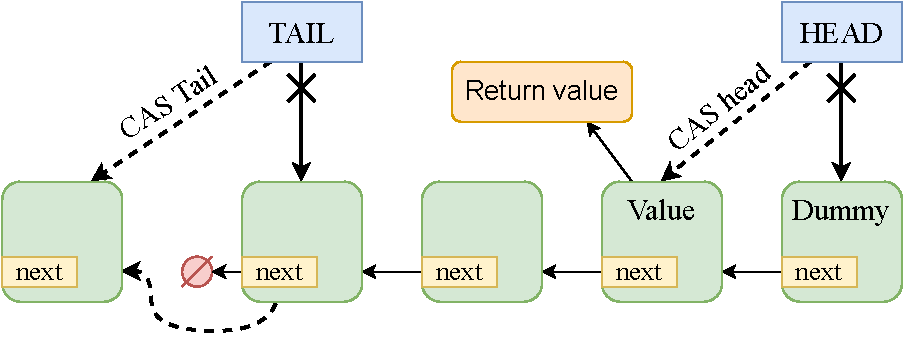
\includegraphics[width=\linewidth]{lock_free_queue}
    \caption{Очередь Майкла - Скотта}
    \label{fig:lock-free-queue}
\end{figure}

Рассмотрим упрощенный код очереди из библиотеки libcds.
Ниже представлена функция enqueue -- добавления в очередь.
Сначала переданное значение кладется в node.
Затем мы пытаемся положить его в хвост очереди.
После получения текущего хвоста указатель продвигается, пока не дойдет до фактического хвоста.
Затем значение ставится в конец очереди, и хвосту присваивается значение вставленного элемента.

\inputminted{c++}{listings/lockFreeQueueEnqueue.cpp}

Для того чтобы достать элемент из очереди (функция dequeue), необходимо, чтобы очередь не была пуста, а также чтобы хвост и голоса были продвинуты.

% TODO: Начать нумеровать листинги?
Код функции приведен ниже.
\inputminted{c++}{listings/lockFreeQueueDequeue.cpp}



	\section{Показатели эффективности параллельной программы}
\subsection{Параллельное ускорение и параллельная эффективность}

Для оценки эффективности параллельной программы принято сравнивать показатели скорости исполнения этой программы при её запуске на нескольких идентичных вычислительных системах, которые различаются только количеством центральных процессоров (или ядер). На практике, однако, редко используют для этой цели несколько независимых аппаратных платформ, т.к. обеспечить их полную идентичность по всем параметрам достаточно сложно. Вместо этого измерения проводятся на одной многопроцессорной (многоядерной) вычислительной системе, в которой искусственно ограничивается количество процессоров (ядер), задействованных в вычислениях. Это обычно достигается одним из следующих способов:

\begin{itemize}
    \itemУстановка аффинности процессоров (ядер).
    \itemВиртуализация процессоров (ядер).
    \itemУправление количеством потоков выполнения.
\end{itemize}

\textbf{Установка аффинности.} Под аффинностью (processor affin\-i\-ty/pin\-ning) понимается указание операционной системе запускать указанный поток/процесс на явно заданном процессоре (ядре). Установить аффинность можно либо с помощью специального системного вызова изнутри самой параллельной программы, либо некоторым образом извне параллельной программы (например, средствами <<Диспетчера задач>> или с помощью команды <<start>> с ключом <</AFFINITY>> в ОС MS Windows, или команды <<taskset>> в ОС Linux). Недостатки этого метода:

\begin{itemize}
    \itemНеобходимость модифицировать исследуемую параллельную программу (при использовании системного вызова изнутри самой программы).
    \itemНевозможность управлять аффиностью на уровне потоков, т.к. обычно ОС позволяет устанавливать аффинность только для процессов (при установке аффиности внешними по отношению к параллельной программе средствами).
\end{itemize}

\textbf{Виртуализация процессоров (ядер).} При создании виртуальной ЭВМ в большинстве специализированных программ (например, VMWare, Virtual\-Box) есть возможность <<выделить>> создаваемой виртуальной машине не все присутствующие в хост-системе процессоры (ядра), а только часть из них. Это можно использовать для имитации тестового окружения с заданным количеством ядер (процессоров). Например, на рисунке~\ref{VirtualBoxNumberCores:image} показано, что для настраиваемой виртуальной машины из восьми доступных физических (и логических) процессоров доступными являются только три.

\begin{figure}[H]
    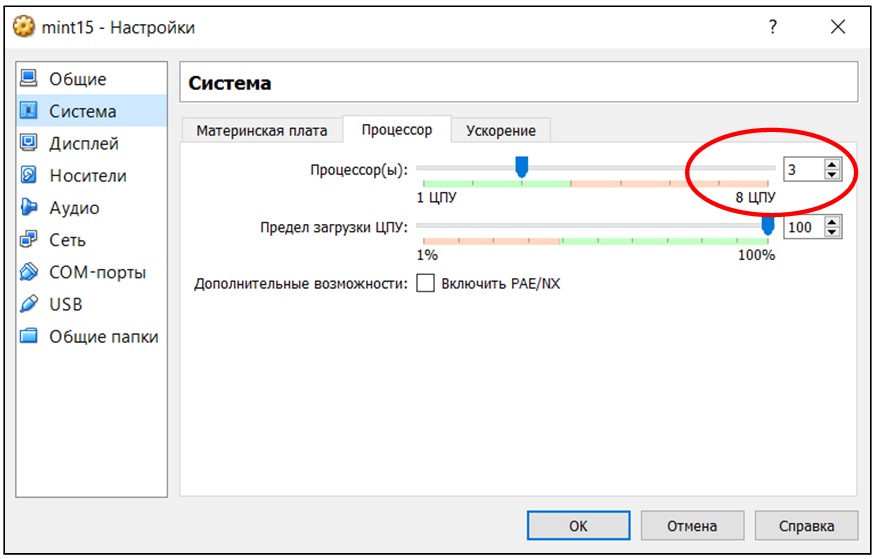
\includegraphics[width=1\linewidth]{VirtualBoxNumberCores}
    \caption{\textit{Выбор количества виртуальных процессоров в Oracle VirtualBox}}
    \label{VirtualBoxNumberCores:image}
\end{figure}

Недостатком описанного подхода являются накладные расходы виртуализации, которые непредсказуемым образом могут сказаться на результатах экспериментального измерения производительности параллельной программы. Достоинством виртуализации (по сравнению с управляемой аффинностью) является более естественное поведение тестируемой программы при использовании доступных процессоров, т.к. ОС не даётся жёстких указаний, что те или иные потоки всегда должны быть <<привязаны>> к заранее заданным процессорам (ядрам) – эта особенность позволяет более точно воспроизвести сценарий потенциального <<живого>> использования тестируемой программы, что повышает достоверность получаемых замеров производительности. 

\textbf{Управление числом потоков.} При создании параллельных программ достаточно часто число создаваемых в процессе работы программы потоков не задаётся в виде жёстко фиксированной величины. Напротив, оно является гибко конфигурируемой величиной p, выбор значения которой позволяет оптимальным образом использовать вычислительные ресурсы той аппаратной платформы, на которой запускается программа. Это позволяет программе <<адаптироваться>> под то число процессоров (ядер), которое есть в наличии на конкретной ЭВМ.

Эту особенность параллельной программы можно использовать для экспериментального измерения её показателей эффективности, для чего параллельную программу запускают при значениях $p = 1, 2, \ldots, n$, где $n$ – это число доступных процессоров (ядер) на используемой для тестирования многопроцессорной аппаратной платформе. Описанный подход позволяет искусственно ограничить число используемых при работе программы процессоров (ядер), т.к. в любой момент времени параллельная программа может исполняться не более чем на $p$ вычислителях. Анализируя измерения скорости работы программы, полученные для различных $p$, можно рассчитать значения некоторых показателей эффективности распараллеливания (см. ниже).

\textbf{Параллельное ускорение (parallel speedup).} В отличие от применяемого в физике понятия величины ускорения как прироста скорости в единицу времени, в программировании под параллельным ускорением понимают безразмерную величину, отражающую прирост скорости выполнения параллельной программы на заданном числе процессоров по сравнению с однопроцессорной системой, т.е.

\begin{equation}
    \label{parallelAcceleration:equation}
    S(p) = \frac{V(p)}{V(1)},
\end{equation}

\noindent где V(p) – средняя скорость выполнения программы на $p$ процессорах (ядрах), выраженная в условных единицах работы в секунду (УЕР/с). Примерами УЕР могут быть количество просуммированных элементов матрицы, количество обработанных фильтром точек изображения, количество записанных в файл байт и т.п.

Считается, что значение $S(p)$ никогда не может превысить $p$, что на интуитивном уровне звучит правдоподобно, ведь при увеличении количества работников, например, в четыре раза невозможно добиться выполнения работы в пять раз быстрее.  Однако, как мы рассмотрим ниже, в экспериментах вполне может наблюдаться сверх-линейное параллельное ускорение при увеличении количества процессоров. Конечно, такой результат чаще всего означает ошибку экспериментатора, однако существуют ситуации, когда этот результат можно объяснить тем, что при увеличении количества процессоров не только кратно увеличивается их вычислительный ресурс, но так же кратно увеличивается объём кэш-памяти первого уровня, что позволяет в некоторых задачах существенно повысить процент кэш-попаданий и, как следствие, сократить время решения задачи.

\textbf{Параллельная эффективность (parallel efficiency).} Хотя величина параллельного ускорения является безразмерной, её анализ не всегда возможен без информации о значении $p$. Например, пусть в некотором эксперименте оказалось, что $S(p)=10$. Не зная значение $p$, мы лишь можешь сказать, что при параллельном выполнение программа стала работать в 10 раз быстрее. Однако если при этом $p=1000$, это ускорение нельзя считать хорошим достижением, т.к. в других условиях можно было добиться почти 1000-кратного прироста скорости работы и не тратить столь внушительные ресурсы на плохо распараллеливаемую задачу. Напротив, при значении $p=11$ можно было бы счесть  величину $S(p)=10$ вполне приемлемой.

Эта проблема привела к необходимости определить ещё один показатель эффективности параллельной программы, который бы позволил получить некоторую оценку эффективности распараллеливания с учётом количества процессоров (ядер). Этой величиной является \textbf{параллельная эффективность}

\begin{equation}
    \label{parallelEffect:equation}
    E(p) = \frac{S(p)}{p} = \frac{V(p)}{p \cdot V(1)}.
\end{equation}

Среднюю скорость выполнения программы $V(p)$ можно измерить следующими двумя \textit{неэквивалентными} методами:

\begin{itemize}
    \item\textbf{Метод Амдала:} рассчитать $V(p)$, зафиксировав объём выполняемой работы (при этом изменяется время выполнения программы для различных $p$).
    \item\textbf{Метод Густавсона-Барсиса:} рассчитать $V(p)$, зафиксировав время работы тестовой программы (при этом изменяется количество выполненной работы для различных $p$).
\end{itemize}

Рассмотрим подробнее каждый из указанных методов в двух следующих подразделах.

\subsection{Метод Амдала}
\label{subsec:amdahl-law}

При оценке эффективности распараллеливания некоторой программы, выполняющей фиксированный объём работы, скорость выполнения можно выразить следующим образом:$\left.V(p)\right|_{w = const} = \frac{w}{t(p)}$, где $w$ – это общее количество УЕР, содержащихся в рассматриваемой программе, $t(p)$ – время выполнения работы w при использовании $p$ процессоров. Тогда выражение для параллельного ускорения примет вид:
\begin{equation}
    \label{eq:amdahl-s-from-p}
    \left.S(p)\right|_{w = const} = \frac{V(p)}{V(1)} = \frac{w}{t(p)} = \frac{w}{t(1)} = \frac{t(1)}{t(p)}.
\end{equation}

Запишем время $t(1)$ следующим образом:
\begin{equation}
    \label{eq:amdahl-s-from-p-2}
    t(1) = t(1) + (k \cdot t(1) - k \cdot t(1)) = k \cdot t(1) + (1 - k) \cdot t(1),
\end{equation}
где $k \in [0,1)$ -- это коэффициент распараллеленности программы, которым мы обозначим долю времени, в течение которого выполняется идеально распараллеленный код внутри рассматриваемой программы. Такой код можно выполнить ровно в $p$ раз быстрее, если количество процессоров увеличить в p раз. Заметим, что коэффициент $k$ никогда не равен единице, т.к. в любой программе всегда присутствует нераспараллеливаемый код, который приходится выполнять последовательно на одном процессоре (ядре), даже если их доступно несколько. Если для некоторой программы $k=0$, то при запуске этой программы на любом количестве процессоров $p$ она будет решаться за одинаковое время.

Учитывая, что в методе Амдала количество работы остаётся неизменным при любом $p$ (т.к. $w=const$), можно утверждать, что значение $k$ не изменяется в проводимых экспериментах, следовательно можем записать:

\begin{equation}
    \label{eq:amdahl-t-from-p}
    t(p) = \frac{k \cdot t(1)}{p} + (1 - k) \cdot t(1),
\end{equation}
где первое слагаемое даёт время работы распараллеленного в p раз идеально распараллеливаемого кода, а второе слагаемое – время работы нераспараллеленного кода, которое не меняется при любом $p$. Подставив формулу~\eqref{eq:amdahl-t-from-p} в~\eqref{eq:amdahl-s-from-p}, получим выражение

\begin{equation}
    \label{eq:amdahl-t-from-p-2}
    \left.S(p)\right|_{w = const} = \frac{t(1)}{t(p)} = \frac{t(1)}{{\displaystyle\frac{k \cdot t(1)}{p}} + (1 - k) \cdot t(1)} = \frac{1}{{\displaystyle\frac{k}{p}} + 1 - k},
\end{equation}
которое перепишем в виде

\begin{equation}
    \label{eq:amdahl-law}
    \left.S(p)\right|_{w=const} = S_A(p) = \left(\frac{k}{p} + 1 - k\right)^{-1},
\end{equation}
более известном как \textbf{закон Амдала} – по имени американского учёного Джина Амдала, предложившего это выражение в 1967 году. До сих пор в специализированной литературе по параллельным вычислениям именно этот закон является основополагающим, т.к. позволяет получить теоретическое ограничение сверху для скорости выполнения некоторой заданной программы при распараллеливании.

График зависимости параллельного ускорения от количества ядер изображен на рисунке~\ref{fig:amdahl-graph}:

\begin{figure}[H]
    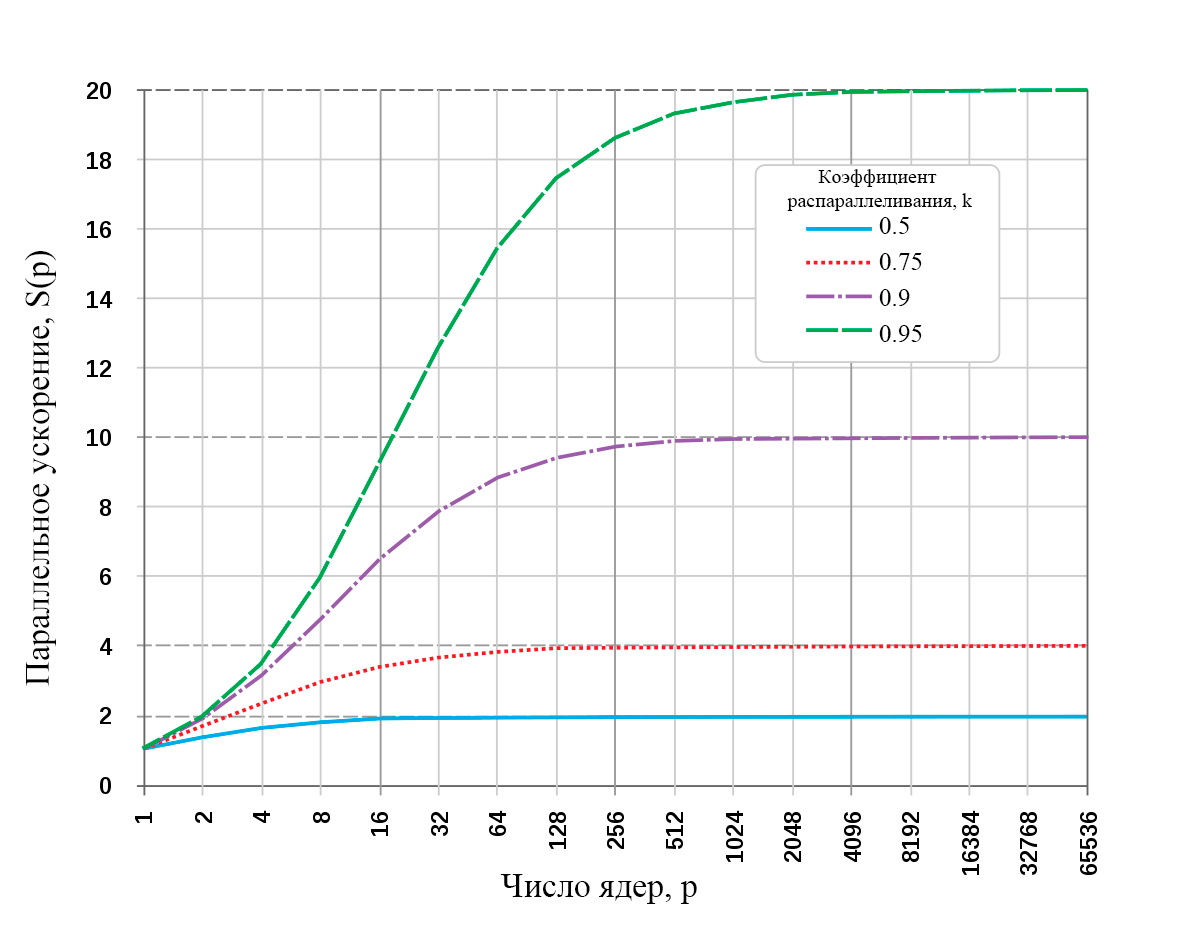
\includegraphics[width=\linewidth]{amdal_plot_ru}
    \caption{График зависимости параллельного ускорения от числа ядер по Амдалу}
    \label{fig:amdahl-graph}
\end{figure}

Отметим, что выражение для расчёта параллельной эффективности при использовании метода Амдала можно получить, объединив формулы~\eqref{eq:parallel-efficiency} и~\eqref{eq:amdahl-law}, а именно:

\begin{equation}
    \label{eq:amdahl-parallel-efficiency}
    E_A(p) = \left(k + p - p \cdot k\right)^{-1}.
\end{equation}

Важным допущением закона Амдала является идеализация физического смысла величины $k$, состоящая в предположении, что идеально распараллеленный код будет давать линейный прирост скорости работы при изменении $p$ от $0$ до $+\infty$ . При решении реальных задач приходится ограничивать этот интервал сверху некоторым конечным положительным значением $p_{max}$ и/или исключать из этого интервала все значения, не кратные некоторой величине, обычно задающей размерность задачи.

Например, код программы, выполняющей конволюционное кодирование независимо для пяти равноразмерных файлов, может давать линейное ускорение при изменении $p$ от $1$ до $5$, но уже при $p=6$, скорее всего, покажет нулевой прирост скорости выполнения задачи (по сравнению с решением при $p=5$). Это объясняется тем, что  конволюционное кодирование, также известное как <<свёрточное>>, является принципиально нераспараллеливаемым при кодировании выбранного блока данных.

\subsection{Метод Густавсона-Барсиса}
\label{subsec:gustafson-barsis-law}

При оценке эффективности распараллеливания некоторой программы, работающей фиксированное время, скорость выполнения можно выразить следующим образом: $\left.V(p)\right|_{t=const}\;=\;\frac {w(p)}t$, где $w(p)$ –- это общее количество УЕР, которые программа успевает выполнить за время $t$ при использовании $p$ процессоров. Тогда выражение~\eqref{eq:parallel-acceleration} для параллельного ускорения примет вид:

\begin{equation}
    \label{eq:gustafson-acceleration}
    \left.S(p)\right|_{t=const} = \frac{V(p)}{V(1)} = \frac{w(p)}{t} : \frac{w(1)}{t} = \frac{w(p)}{w(1)}.
\end{equation}

Запишем количество работы $w(1)$ следующим образом:

\begin{equation}
    \label{eq:gustafson-work}
    w(1) = w(1) + (k \cdot w(1) - k \cdot w(1)) = k \cdot w(1) + (1 - k) \cdot w(1),
\end{equation}
где $k\in[0,1)$ -- это уже упомянутый ранее коэффициент распараллеленности программы. Тогда первое слагаемое можно считать количеством работы, которая идеально распараллеливается, а второе –- количество работы, которую распараллелить не удается при добавлении процессоров (ядер).

При использовании $p$ процессоров количество выполненной работы $w(p)$ очевидно станет больше, при этом оно  будет состоять из двух слагаемых: 

\begin{itemize}
    \itemколичество нераспараллеленных условных единиц работы $(1-k) \cdot w(1)$, которое не изменится по сравнению с формулой~\eqref{eq:gustafson-work}.
    \itemколичество распараллеленных УЕР, объём которых увеличиться в $p$ раз по сравнению с формулой~\eqref{eq:gustafson-work}, т.к. в работе будет задействовано $p$ процессоров вместо одного.
\end{itemize}

Учитывая сказанное, получим следующее выражение для $w(p)$:

$w(p) = p \cdot k \cdot w(1) + (1 - k) \cdot w(1),$ тогда с учетом формулы~\eqref{eq:gustafson-acceleration} получим: $\frac{w(p)}{w(1)} = \frac{p \cdot k \cdot w(1) + (1 - k) \cdot w(1)}{w(1)}$, что позволяет записать:
\begin{equation}
    \left.S(p)\right|_{t=const} = S_{GB}(p) = p \cdot k + 1 - k.
\end{equation}

Приведённое выражение называется \textbf{законом Густавсона-Барсиса}, который Джон Густавсон и Эдвин Барсис сформулировали в 1988 году. 

\subsection{Модификация закона Амдала (по проф. Бухановскому)}
\label{subsec:amdahl-law-bukhanovskiy-modification}


В реальных вычислительных системах ОС тратит ресурсы на создание и удаление новых потоков. Время, затраченное на эти операции, не учитывается в законе Амдала. Параллельное ускорение $S(p)$ зависит от числа ядер и доли распараллеливаемых операций, но не зависит от числа последних. Выведем формулу, в которой число операций, для которых необходимо создать поток, будет учитываться.

Пусть $N$ -- число распараллеливаемых операций, $M$ -- число нераспараллеливаемых операций, $t_c$ -- время выполнения одной операции, $p$ -- число вычислителей (ядер), $T_i$ -- время выполнения программы при использовании $i$ параллельных потоков на $i$ вычислителях, $\alpha$ -- некий масштабирующий коэффициент, инкапсулирующий в себе время, требуемое на создание, удаление потока и прочие накладные операции. 
По формуле~\eqref{eq:amdahl-s-from-p}, $S(p) = {T_1} / {T_p}$.

Найдем сначала $T_1$. Так как это код выполняется линейно, то время, затраченное на его выполнение, будет равно числу операций, умноженному на время выполнения одной операции: $T_1 = t_c \cdot (N + M)$.

Время выполнения распараллельнной программы $T_p$ включает в себя время на создание потока: $t_c \cdot \alpha \cdot (p - 1) \cdot N$ (нужно создать $(p - 1)$ новых потоков, так как главный поток уже создан, и для каждого затратить какое-то время $\alpha$), время работы распараллеливаемоего кода на всех ядрах: $(t_c \cdot N) / {p}$ и время работы нераспараллеливаемого кода $t_c \cdot M$. Итого, разделив $T_1$ на $T_p$, получим формулу закона Амдала по проф. А.В. Бухановскому:

\begin{equation}
    \label{eq:amdahl-bukhanovskiy}
    S(p,N) = \frac{T_1}{T_p} = \frac{N + M}{\alpha \cdot (p - 1) \cdot N + \displaystyle\frac{N}{p} + M}.
\end{equation}

Из формулы~\eqref{eq:amdahl-bukhanovskiy} видно, что с ростом числа ядер после определенного предела $S(p,N)$  не будет расти как в законе Амдала, так как будет тратиться много времени на создание новых потоков. На рисунке~\ref{fig:amdahl-bukhanovskiy} наглядно видно, что $S(p,N)$ уменьшается при большом числе потоков и становится заметно меньше $S(p)$ по Амдалу даже при небольшом значении $\alpha$.

\begin{figure}[H]
    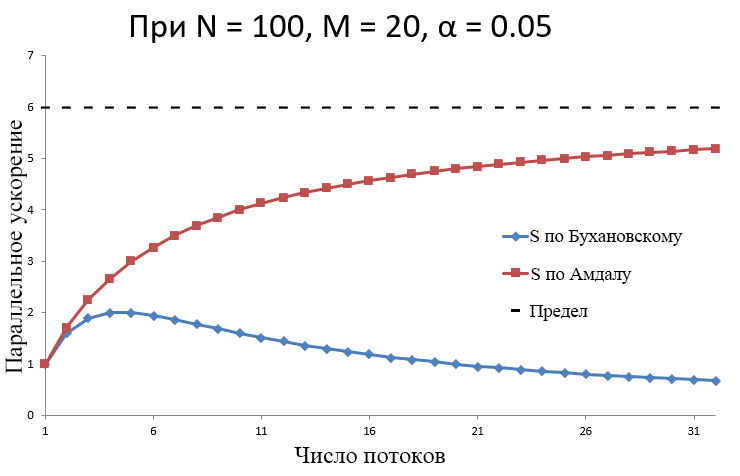
\includegraphics[width=\linewidth]{GraphAmdalBuhunovsky} % TODO: rename file
    \caption{График зависимости параллельного ускорения от числа потоков}
    \label{fig:amdahl-bukhanovskiy}
\end{figure}

\subsection{Измерение времени выполнения параллельных программ}
\label{subsec:execution-time-measurement}

\textbf{Инструменты измерения времени.} Измерение времени работы программы в языке С не является сложной проблемой, однако при параллельном программировании возникает ряд специфических сложностей при выполнении этой операции. Далеко не все функции, пригодные для измерения времени работы последовательной программы, подойдут для измерения времени работы многопоточной программы. 

Например, если в однопоточной программе для измерения времени работы участка кода использовать функции ctime или localtime, то они успешно справятся с поставленной задачей. Однако после распараллеливания этого участка кода возможно возникновение трудно идентифицируемых проблем с неправильным измерением времени, т.к. обе указанные функции имеют внутреннюю static-переменную, которая при попытке изменить её одновременно несколькими потоками может принять непредсказуемое значение.

С целью решить описанную проблему в некоторых C-компиляторах (например, gcc) были реализованы потокобезопасные (thread-safe, reen\-trant) версии этих функций: ctime\_r и localtime\_r. К сожалению, эти функции доступны не во всех компиляторах. Например, в компиляторе Visual Studio аналогичную проблему решили использованием функций с совсем иными именами и API: Get\-Tick\-Count, Get\-Local\-Time, Get\-System\-Time. Перечислим для полноты изложения некоторые другие gcc-функции, которые также позволяют измерять время: time, get\-r\-usage, gm\-time, get\-time\-of\-day.

Ещё одна стандартная С-функция clock также не может быть использована для измерения времени выполнения многопоточных программ. Однако причина этого не в отсутствии реентерабельности, а в особенностях способа, которым эта функция рассчитывает прошедшее время: clock возвращает число тиков процессора, которые были выполнены при работе программы суммарно всеми её потоками. Очевидно, что это число остается почти неизменным при выполнении программы разным числом потоков (<<почти>>, т.к. накладные расходы на создание, удаление и управление потоками предлагается в целях упрощения изложения считать несущественными).

В итоге оказалось, что удовлетворительного \textit{кросс-платформенного} решения для потокобезопасного измерения времени с высокой точностью (до микросекунд) средствами чистого языка С пока не существует. Проблему, однако, можно решить, используя сторонние библиотеки, выбирая те из них, которые имеют реализацию на целевых платформах.

Выгодно выделяется среди таких библиотек система OpenMP, которая реализована в абсолютном большинстве современных компиляторов для всех современных операционных систем. В OpenMP есть две функции для измерения времени: omp\_get\_wtime и omp\_get\_wtick, которые можно использовать в С-программах, если подключить заголовочный файл omp.h и при компиляции указать нужный ключ (например, в gcc это ключ <<-fopenmp>>).

\textbf{Погрешность измерения времени.} Другим интересным моментом при измерении времени работы параллельной программы является способ, с помощью которого исследователь исключает из замеров различные случайные погрешности, неизбежно возникающие при эксперименте в работающей операционной системе, которая может начать процесс обновления или оптимизации, не уведомляя пользователя. Общепринятыми является способ, при котором исследователь проводит не один, а сразу N экспериментов с параллельной программой, не меняя исходные данные. Получается N замеров времени, которые в общем случае будут различными вследствие различных случайных факторов, влияющих на проводимый эксперимент. Далее чаще всего используется один из следующих методов:

\begin{enumerate}
    \item\textit{Расчёт доверительного интервала:} с учётом всех N измерений рассчитывается доверительный интервал, например, с помощью метода Стьюдента.
    \item\textit{Поиск минимального замера:} среди N измерений выбирается наименьшее и именно оно используется в качестве окончательного результата.
\end{enumerate}

Первый метод даёт корректный результат, только если ошибки замеров распределены по нормальному закону. Чаще всего это так, поэтому применение метода оправдано и также позволяет получить дополнительную информацию о возможном применении тестируемой программы в живых условиях работающей ОС.

Второй метод не предъявляет требований к виду закона распределения ошибки измерений и этим выгодно отличается от предыдущего. Кроме того, при больших N выбор минимального замера позволит с большой вероятностью исключить из эксперимента все фоновые влияния операционной системы и получить в качестве результата точное измерение времени работы программы в идеальных условиях. 

\textbf{Практический пример.} Сравним на примере описанные выше методы избавления от погрешности экспериментальных замеров времени. Будем измерять накладные расходы OpenMP на создание и удаление потоков следующим образом:

\inputminted{c++}{listings/OpenMPExampleTimeMeasurement.cpp}

В строке 2 мы даём OpenMP указание, чтобы при входе в параллельную область, расположенную далее в программе, было создано i потоков. Если не давать этого указания, OpenMP создаст число потоков по числу доступных в системе вычислителей (ядер или логических процессоров). В строке 4 мы запускаем параллельную область программы, OpenMP создаёт i потоков. В строке 5 мы даём указание выполнять последующую простейшую инструкцию лишь в одном потоке (остальные потоки не будут делать никакой работы. Это нужно, чтобы в замеряемое время работы попали только расходы на создание/удаление потоков, а все прочие расходы терялись бы на их фоне. В строке 6 заканчивается параллельная область, OpenMP удаляет из памяти i потоков. Более подробное описание использованных команд OpenMP можно найти в разделе~\ref{OpenMP:section} \textit{<<Технология OpenMP>>} данного учебного  пособия.

Эксперименты с приведённой программой проводились на компьютере с процессором Intel Core i5 (4 логических процессора) с 8 гигабайт ОЗУ в операционной системе Debian Wheezy. Опытным путём было выявлено, что использованная операционная система на доступной аппаратной платформе не может создать более 381 потока в OpenMP-программе (этим объясняется значение в строке 1). Было проведено в общей сложности N=100 экспериментов, результаты которых обрабатывались каждым из двух описанных методов. Полученные результаты приведены на рисунке~\ref{fig:openmp-creating-threads-overhead}.

\begin{figure}[H]
    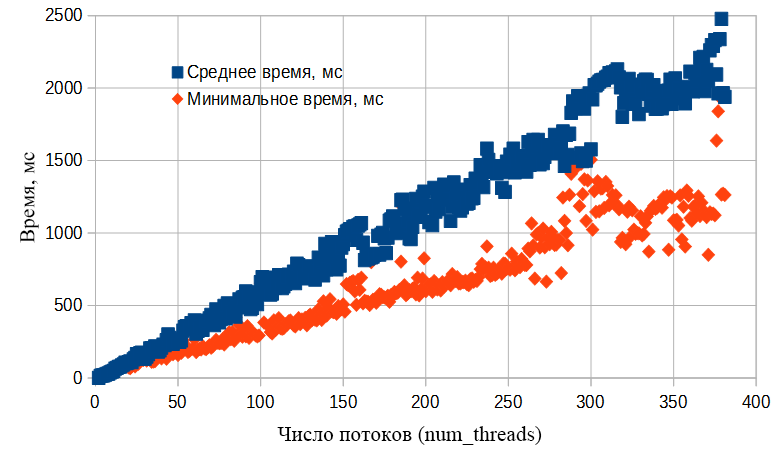
\includegraphics[width=1\linewidth]{OpenMPExpensesOnCreatingThreads}
    \caption{Результаты измерения накладных расходов OpenMP при создании и удалении потоков}
    \label{fig:openmp-creating-threads-overhead}
\end{figure} 

По оси ординат откладывается измеренная величина (T2 - T1) в миллисекундах, по оси абсцисс – значения переменной i, означающие число создаваемых потоков. Верхний график, состоящий из синих квадратов, показывает усреднённую величину (T2 - T1) по 100 проведённым экспериментам. Доверительный интервал при этом не показан, т.к. он загромождал бы график, не добавляя информативности, однако ширина доверительного интервала с уровнем доверия 90\% приблизительно соответствует разбросу по вертикали квадратов верхнего графика для соседних значений i.

Нижний график, состоящий из ромбов, представляет собой минимальные из 100 проведённых замеров величины (T2 -  T1) для указанных на оси абсцисс значений i. Видим, что даже большого числа экспериментов оказалось недостаточно, чтобы нижний график имел бы гладкую непрерывную структуру без заметных флуктуаций.

\subsection{Профилирование параллельных программ}
\label{subsec:profiling-parallel-programs}

Профилирование -- сбор характеристик работы программы, таких как время выполнения отдельных фрагментов (обычно подпрограмм), число верно предсказанных условных переходов, число кэш-промахов и т. д. Инструмент, используемый для анализа работы, называют профилировщиком или профайлером.

\textbf{Intel Parallel Amplifier.} Этот инструмент позволяет найти те участки кода, которые наиболее часто исполняются на процессоре. Также он позволяет оценить масштабируемость вашего параллельного приложения. И если есть какие-то проблемы с масштабируемостью, то найти те участки кода, которые этой масштабируемости мешают. В Intel Parallel Amplifier представлено три вида анализа:

\begin{enumerate}
    \item Hotspot-анализ -- Позволяет узнать где тратятся вычислительные ресурсы, а также изучить стек вызовов.
    \item Concurrency-анализ -- Происходит оценка эффективности параллельного кода.
    \item Lock\&Wait-анализ -- Указывает на те места, где программа плохо распараллеливается.
\end{enumerate}

Пройдя все эти этапы анализа, пользователь должен сформировать для себя определенное понимание поведения приложения в плане загрузки микропроцессора и эффективного использования его ресурсов. Далее на основе полученных результатов, можно решать дальнейшие шаги оптимизации программы.

Больше информации о Intel Parallel Amplifier можно посмотреть в~\cite{IntelAmplifier}.
% \url{https://www.ixbt.com/soft/intel-parallel-amplifier.shtml}.


	\section{Практические аспекты параллельного программирования}
\subsection{Отладка параллельных программ}

Средства отладки параллельных программ встроены в большинство популярных интегрированных сред разработки (IDE), например: Visual Studio, Eclipse CDT, Intel Parallel Studio и т.п. Эти средства включают в себя удобную визуализацию временных диаграмм исполнения потоков, автоматический поиск подозрительных участков программы, в которых могут наблюдаться гонки данных и взаимоблокировки.

Несмотря на эффективность существующих инструментов отладки, при работе в дебаггере (debugger) с параллельной программой возникают существенные затруднения, т.к. для своего корректного функционирования отладчик добавляет в машинный код исходной параллельной программы дополнительные инструкции, которые изменяют временную диаграмму выполнения потоков по отношению друг к другу. Это может приводить к ситуациям, когда при тестировании программы в отладчике не наблюдаются гонки данных и взаимоблокировки, которые при запуске Release-версии программы проявятся в полной мере.

Также при отладке многопоточной программы следует иметь в виду, что её поведение (как при штатной работе, так и при отладке) может существенным образом различаться при использовании одноядерного и многоядерного процессора. При запуске нескольких потоков на одноядерной машине они будут выполняться в режиме разделения времени, т.е. последовательно. Значит, в этом случае не будут наблюдаться многие проблемы с совместным доступом к памяти и обеспечением когерентности кэшей, присущие многоядерным системам. Кроме того, при отладке программы на одноядерной системе программист может использовать неявные приёмы обеспечения последовательности выполнения операций. 

Например, программист может некорректно предполагать, что при выполнении высокоприоритетного потока низкоприоритетный поток не может завладеть процессором. Это предположение корректно только в одноядерной системе, ведь при наличии нескольких ядер и малом количестве высокоприоритетных потоков вполне может наблюдаться ситуация, когда низкоприоритетный поток завладеет одним из ядер, при одновременной работе высокоприоритетного потока на соседнем ядре.

\subsection{Менеджеры управления памятью для параллельных программ}

При вызове функций malloc/free в однопоточной программе не возникает проблем даже при довольно высокой интенсивности вызовов одной из них. Однако в параллельных программах эти функции могут стать узким местом, т.к. при их одновременном использовании из нескольких потоков происходит блокировка общего ресурса (менеджера управления памятью), что может привести к существенной деградации скорости работы многопоточной программы.

Получается, что несмотря на формальную потокобезопасность стандартных функций работы с памятью, они могут стать потоконеэффективными при очень интенсивной работе с памятью нескольких параллельно работающих потоков.

Для решения этой проблемы существует ряд сторонних программ, называющихся <<Менеджер управления памятью (МУП)>> (Memory Al\-lo\-ca\-tor), как платных, так и бесплатных с открытым исходным кодом. Каждое из них обладает своими достоинствами и недостатками, которые следует учитывать при выборе. Перечислим наиболее распространённые МУП с указанием ссылок на официальные сайты:

\begin{itemize}
    \item tcmalloc: \url{http://goog-perftools.sourceforge.net/doc/tcmalloc.html}
    \item ptmalloc: \url{http://www.malloc.de/malloc/ptmalloc3-current.tar.gz}
    \item dmalloc: \url{http://dmalloc.com}
    \item HOARD: \url{http://www.hoard.org}
    \item nedmalloc: \url{http://www.nedprod.com/programs/portable/nedmalloc}
    \item jemalloc: \url{http://jemalloc.net}
    \item mimalloc: \url{https://github.com/microsoft/mimalloc}
\end{itemize}

Перечисленные МУП разработаны таким образом, что ими можно <<незаметно>> для параллельной программы подменить стандартные МУП библиотеки libc языка С. Это значит, что выбор конкретного МУП никак не влияет на исходный код программы, поэтому общая практика использования сторонних МУП такова: параллельная программа изначально создаётся с использованием МУП libc, затем проводится профилирование работающей программы, затем при обнаружении узкого места (bottleneck) в функциях malloc/free принимается решение заменить стандартный МУП одним из перечисленных.

Также стоит отметить, что некоторые технологии распараллеливания (например, Intel TBB) уже имеют в своём составе специализированный МУП, оптимизированный для выполнения в многопоточном режиме.

\subsection{Библиотека Intel IPP}
\label{IPP:section}

\textbf{Оптимизация типовых задач обработки данных.} Существует немногочисленное количество высокопроизводительных библиотек, состоящих из набора низкоуровневых API для обработки данных: изображений, сигналов, матриц.

Одной из таких библиотек является <<Intel IPP>>\footnote{Intel Integrated Performance Primitives}, реализующая следующие функции:
\begin{itemize}
    \itemКодирование и декодирование видео.
    \itemКодирование и декодирование аудио.
    \itemКомпьютерное зрение.
    \itemКриптография.
    \itemСжатие данных.
    \itemПреобразование цвета.
    \itemОбработка изображения.
    \itemТрассировка луча/визуализация.
    \itemОбработка сигналов.
    \itemКодирование речи.
    \itemРаспознавание речи.
    \itemОбработка строк.
    \itemВекторная/матричная математика.
\end{itemize}

Для использования функций данной библиотеки необходимо в исходном коде подключить заголовочный файл IPP: 
\mint{c++}{#include <ipp.h>}

Рассмотрим пример программы которая вычисляет модуль синуса каждого элемента массива:

\begin{minted}{c++}
for (int i=0; i<N; i++){
    array[i] = abs(sin(array[i]));
}
\end{minted}

Теперь воспользуемся функциями IPP, тогда наша программа будет выглядеть так:

\begin{minted}{c++}
ippsSin_64f_A21(array, array, N);
ippsAbs_64f_A21(array, array, N);
\end{minted}

Благодаря использованию данных функция, программа стала компактнее и быстрее.

Более подробно об использовании функций IPP можно узнать из официальной документации~\cite{IppPrimitives}.
% Все об использовании функций IPP можно узнать из официальной документации~\cite{IppPrimitives}.
% \url{https://software.intel.com/content/www/us/en/develop/documentation/ipp-dev-reference/top.html}.

\subsection{Технология OpenMP}
\label{OpenMP:section}

\textbf{Краткая характеристика технологии.} Первая версия стандарта \linebreak OpenMP появилась в 1997 году при поддержке крупнейших IT-компаний мира (Intel, IBM, AMD, HP, Nvidia и др.). Целью нового стандарта было предложить кроссплатформенный инструмент для распараллеливания, который был бы более высокоуровневый, чем API управления потоками, предлагаемые операционной системой. На данный момент OpenMP стандартизована для трёх языков программирования: С, С++ и Фортран.

\textbf{Поддержка компиляторами.} Абсолютное большинство существующих современных компиляторов С/С++ поддерживают OpenMP версии 2.0 (например, как gcc, так и Visual Studio). Однако не все компиляторы поддерживают последнюю версию OpenMP 5.2, поэтому далее при изложении материала будет в качестве <<общего знаменателя>> использоваться технология OpenMP 2.0.

OpenMP определяет набор директив препроцессору, которые дают указание компилятору заменить следующий за ними исходный код на его параллельную версию с помощью доступных компилятору средств, например с помощью POSIX Threads в Linux или Windows Threads в операционных системах Microsoft. Для корректной трансляции директив необходимо при компиляции указать специальный ключ, значение которого зависит от компилятора (примеры приведены в таблице~\ref{compilerOpenMP:table}).

\begin{table}[H]
    \caption{Ключи компиляторов для запуска OpenMP}
    \label{compilerOpenMP:table}
    \centering
    \begin{tabular}{|c|c|}
        \hline
        \thead{Название компилятора} & \thead{Ключ компилятору для \\ включения OpenMP} \\ \hline
        gcc                          & -fopenmp \\ \hline
        icc (Intel C/C++ compiler)   & -qopenmp \\ \hline
        Sun C/C++ compiler           & -xopenmp \\ \hline
        Visual Studio C/C++ compiler & /openmp  \\ \hline
        PGI (Nvidia C/C++ compiler)  & -mp      \\ \hline
    \end{tabular}
\end{table}

Помимо препроцессорных директив, OpenMP определяет набор библиотечных функций, для вызова которых в исходном коде потребуется подключить заголовочный файл OpenMP:
\mint{c++}{#include <omp.h>}

\textbf{Отличительные особенности.} Среди прочих технологий распараллеливания OpenMP выделяется следующими важными и характеристиками:

\begin{itemize}
    \itemИнкрементное распараллеливание.
    \itemОбратная совместимость.
    \itemВысокий уровень абстракций.
    \itemНизкий коэффициент трансформации.
    \itemПоддержка крупнейшими IT-гигантами. 
    \itemАвтоматическое масштабирование.
\end{itemize}

\textit{Инкрементное распараллеливание.}  OpenMP позволяет распараллеливать существующую последовательную программу с помощью небольших итераций-правок, на каждой из которых будет достигаться всё больший коэффициент распараллеленности программы. Эта особенность является уникальной, т.к. большинство других технологий предполагают существенное изменение структуры распараллеливаемой программы уже на первом этапе процесса распараллеливания, т.е. первая работоспособная параллельная версия программы появляется после длительного процесса отладки и программирования новых компонентов, которые неизбежно добавляются при распараллеливании. OpenMP лишён этого недостатка.

\textit{Обратная совместимость.} Большинство программных технологий развиваются с обеспечением обратной совместимости (back\-ward com\-pat\-i\-bil\-i\-ty), когда более новая версия программы поддерживает работоспособность старых файлов. Термин \textit{<<прямая совместимость>>} (forward compatibility) имеет противоположный смысл: файлы, созданные в программе новой версии, остаются работоспособными при использовании старой версии программы. В случае OpenMP это проявляется в том, что распараллеленная программа будет корректно скомпилирована в однопоточном режиме даже на старом компиляторе, который не поддерживает OpenMP. Важно отметить, что прямая совместимость обеспечивается, если при распараллеливании не используются библиотечные функции OpenMP, а присутствуют только препроцессорные директивы. При наличии библиотечных функций для обеспечения обратной совместимости потребуется написать функции-заглушки в файле <<omp.h>> (некоторые компиляторы умеют генерировать эти заглушки при использовании специального ключа).

\textit{Высокий уровень абстракций.} Всего лишь одна единственная препроцессорная директива OpenMP (любая, но корректная) после обработки компилятором приводит к существенной трансформации исходной программы с добавлением большого количества новой логики, отвечающей за определение доступного в системе числа процессоров, за запуск и уничтожение потоков, за распределение работы между потоками и т.п. Все эти операции OpenMP берёт на себя, взамен программист получает набор очень высокоуровневых инструментов распараллеливания. У высокоуровневых языков есть и традиционный недостаток: в OpenMP отсутствует возможность изменить некоторые внутренние детали работы с потоками (например, нельзя установить аффинность потоков или уменьшить накладные расходы на создание/удаление потоков).

\textit{Низкий коэффициент параллельной трансформации (КПТ).} При распараллеливании существующей последовательной программы приходится вносить в неё достаточно большое число изменений. Пусть КПТ -- это отношение строк нового программного кода, который добавился в результате распараллеливания, к общему числу строк кода в программе. В OpenMP КПТ обычно существенно ниже, чем у большинства других технологий распараллеливания. Это объясняется высоким уровнем абстракции языка OpenMP (см. предыдущий пункт). 

\textit{Поддержка крупнейшими  IT-гигантами.} Уже при разработке Open\-MP о его поддержке заявили крупнейшие игроки IT-мира. Это обеспечило не только высокое качество разработки стандарта, но и наличие готовых реализаций стандарта в популярных компиляторах. Несмотря на прошедшие два десятка лет, OpenMP не растерял приверженцев, и поддержка новейших версий OpenMP с достаточно малой задержкой появляется в компиляторах. Например, при текущей версии стандарта OpenMP 5.2 наиболее популярные компиляторы уже поддерживают версию OpenMP 4.0. Исключением является только компания Microsoft. Их компилятор вот уже несколько версий неизменно поддерживает только OpenMP 2.0. 

\textit{Автоматическое масштабирование.}  Низкоуровневые технологии распараллеливания (POSIX Threads, OpenCL) предлагают программисту вручную управлять числом создаваемых потоков при выполнении параллельной работы. Это обеспечивает возможность гибко управлять и настраивать процесс создания потоков в зависимости от числа доступных системе процессоров (ядер), но при этом требует от программиста большое количество неавтоматизируемой работы. В OpenMP управление масштабированием происходит в автоматическом режиме, т.е. OpenMP сам запрашивает у операционной системы число доступных процессоров и выбирает число создаваемых потоков. Но при необходимости OpenMP оставляет возможность устанавливать требуемое число потоков вручную.

\textbf{Примеры OpenMP-программ.} Рассмотрим ниже простейшие примеры работающих параллельных программ, начиная с традиционного для программирования примера <<Hello, World>>:
\inputminted{c++}{listings/OpenMPExample1.cpp}

Результатом работы будет выведенное несколько раз в консоль сообщение. Число сообщений определяется числом логических процессоров, доступных системе (например, при использовании технологии HyperThreading при двух ядрах число логических процессоров будет равно четырём). 

Действие директивы pragma распространяется на следующий за ней исполняемый блок. В данном случае это вызов функции printf, но можно было бы заключить произвольное число операций в фигурные скобки, чтобы расширить исполняемый блок:
\inputminted{c++}{listings/OpenMPExample2.cpp}

В этой программе заключенный в фигурные скобки блок операций выполняется одновременно на нескольких ядрах. При этом в строке 5 процессору даётся указание выполнить операцию <<i++>> атомарно, т.е. не параллельно, а последовательно каждым из потоков. 

С одной стороны, это приводит к тому, что операция инкремента перестаёт быть распараллеленной, что снижает скорость многоядерного выполнения. С другой стороны, директива atomic в данном случае необходима, т.к. иначе могла бы возникнуть сложно обнаружимая проблема с гонкой данных, проявляющаяся в конфликте при записи данных в общую область памяти одновременно несколькими потоками в переменную i. Заметим, что директива atomic может применяться только для однострочных простых команд присваивания. 

Для изоляции более сложных составных команд с возможным вызовом пользовательских и системных функций следует использовать директиву critical, которая допускает (в отличие от директивы atomic) возможность расширения своей области действия на блок операций, заключённый в фигурные скобки, при этом каждая critical-секция может иметь имя, позволяющее сгруппировать разные критические секции по этому имени, чтобы предотвратить появление единой распределённой по всей программе критической секции:
\inputminted{c++}{listings/OpenMPExample3.cpp}

В этом случае функция printf в строке 4 выполняется всеми потоками параллельно, что может привести к перемешиванию выводимых символов. Напротив, функция printf в строке 8 выполняется потоками строго по очереди, что предотвращает возможные конфликты между ними, однако замедляет выполнение программы из-за искусственного ограничения коэффициента распараллеленности.

Приведём пример распараллеливания программы, содержащей последовательный вызов функций run\_function1 и run\_function2, которые не зависят друг от друга (т.е. не используют общих данных и результаты работы одной не влияют на результаты работы другой) и поэтому допускающих удобное \textit{распараллеливание по инструкциям} в чистом виде:

\inputminted{c++}{listings/OpenMPExample4.cpp}

Рассмотрим пример распараллеливания цикла с использованием OpenMP. Пусть в каждую ячейку одномерного массива нужно записать индекс этой ячейки, возведённый в шестую степень:

\inputminted{c++}{listings/OpenMPExample5.cpp}

Пусть указанная программа выполняется на двухъядерном процессоре. Тогда первый процессор рассчитает значения с a[0] по a[4], второй процессор – значения с a[5] по a[9]. Видимо, что при записи в массив процессору не мешают друг другу, т.к. работают с разными частями массива. Попробуем оптимизировать предыдущий вариант, сократив число операций умножения для возведения в шестую степень:

\inputminted{c++}{listings/OpenMPExample6.cpp}

В указанном случае программа будет корректно работать только при наличии одного процессора (ядра). При наличии нескольких ядер будет наблюдаться состояние гонки данных при одновременной записи нового значения в переменную tmp (строка 4) несколькими потоками, в результате массив будет заполнен некорректно. Например, пусть первый поток, выполняющий итерацию $i=2$, записал в tmp число 8. Теперь при вычислении a[2] поток попытается записать число $8*8$, однако если до начала строки 5 успеет вклиниться второй поток, работающей с итерацией $i=7$, то значение tmp превратится в $7*7*7$, а значение a[2], рассчитываемое первым потоком, превратится в $7^6$ ($7*7*7$ в квадрате), вместо положенных 64. Исправим допущенную ошибку следующим образом:

\inputminted{c++}{listings/OpenMPExample7.cpp}

В директиве препроцессору появился новый элемент: private. Этот элемент задаёт через запятую перечень локальных (приватных) для каждого потока переменных. В данном случае такая переменная одна: tmp. Другой равноценный способ исправить ошибку -- это перенести объявление переменной <<int tmp>> внутрь параллельной области, что заставить OpenMP считать эту переменную локальной для каждого потока. Может возникнуть вопрос, почему в перечень локальных переменных не добавлена i. Ответ не очевиден: OpenMP по умолчанию считает переменную распараллеливаемого цикла локальной.

Любая переменная, объявленная внутри параллельной области, считается в OpenMP локальной, поэтому такие переменные не нужно указывать в списке. Любая переменная, объявленная вне этой области, является глобальной (в нашем случае глобальной переменной является указатель на массив $a$). Но если требуется явным образом указать на глобальность переменной, следует рядом с командой private использовать команду \code{shared(x, ...)}, где x задаёт список глобальных переменных.

Рассмотрим пример, в котором нужно рассчитать сумму и для дальнейшего исполнения формировать массив элементов следующего ряда: $\{1^i, 2^i, 3^i, 4^i, 5^i\}$ для различных значений $i$, например: $i = 1, 2, 3$. Приведём ниже решение поставленной задачи, но умышленно допустим в ней ошибку:

\inputminted{c++}{listings/OpenMPExample8.cpp}

В строке 2 происходит запуск параллельной области, но программист забывает указать, что переменные j и массив tmp должны быть локальными для каждого треда. Действительно, в строке 4 происходит инкремент общей для потоков переменной j, который выполняется всеми потоками одновременно. В этой ситуации потоки могут помешать друг другу, переписав чужое значение j. Исправим обе ошибки следующим образом:

\inputminted{c++}{listings/OpenMPExample9.cpp}

Видим, что теперь переменная j явным образом обозначена локальной (private). С массивом tmp решение другое – он весь помещается внутрь параллельной области (т.е. у каждого потока будет свой собственный не зависимый от других экземпляр массива tmp). Почему же нельзя было просто указать переменную tmp в перечне команды private, как это было сделано для j? Ответ связан со спецификой языка С: переменная tmp является указателем, который при работе цикла не меняется, но меняется содержимое памяти, на которое указывает tmp. Это значит, что указывание tmp в качестве private-переменной не решило бы проблему с гонками данных, т.к. все потоки получили бы один и тот же адрес tmp и мешали бы друг другу, записывая новые значения по этому адресу.

Рассмотрим ещё одну типичную для параллельного программирования ошибку. Следующая программа считает сумму чисел от 1 до 100:

\inputminted{c++}{listings/OpenMPExample10.cpp}

Переменная sum является глобальной, поэтому при попытке записать в неё новое значение потоки будут мешать друг другу. Чтобы исправить ошибку, нам придётся использовать локальную для каждого потока сумму, а затем потребуется сложить все эти локальные суммы:

\inputminted{c++}{listings/OpenMPExample11.cpp}

Видим начало параллельной области в строке 2 – именно в этом месте OpenMP создаёт несколько потоков. В строке 6 новые потоки не создаются (т.к. отсутствует ключевое слово parallel), но входящие в цикл потоке делят итерации между собой, а не выполняют каждый все итерации целиком. В строке 8 рассчитавший свою частичную сумму поток пытается прибавить эту сумму к общей сумме. Это приходится делать с помощью директивы atomic, которая гарантирует, что потоки не будут мешать друг другу при перезаписи sum. 

Ещё один сложный момент – это повторная инициализация переменной sum\_private в строке 4: необходимость в этом возникает, т.к. OpenMP не инициализирует локальные переменные, даже если есть глобальные переменные с идентичными именами. Подобное решение призвано уменьшить накладные расходы на копирование переменных.

Описанный подход является работоспособным, однако он почти не используется на практике, т.к. стандарт OpenMP для целого класса подобных задач предлагает более высокоуровневое и простое решение. Оно состоит в использовании команды reduction:

\inputminted{c++}{listings/OpenMPExample12.cpp}

Команда reduction помечает перечисленный переменные как локальные, а в конце параллельной области все локальные переменные объединяет (агрегирует) в одну глобальную переменную с тем же именем, используя указанную операцию. В нашем случае операцией является суммирование. Но OpenMP допускает вместо знака <<+>> использовать <<*>>, <<->>, <</>>, а в последних версиях и функции, написанные разработчиками. Важно, что reduction, кроме прочего, выполняет инициализацию переменных не значениями исходных глобальных переменных, а наиболее соответствующими логики агрегации значениями: например, при суммировании переменная инициализируется нулём, а при умножении – единицей.

При распараллеливании цикла может оказаться, что итерации не\-рав\-но\-цен\-ны по количеству выполняемой работы между собой. Это может привести к тому, что один поток справится с выделенной частью итераций намного быстрее второго потока и будет простаивать. Для решения этой проблемы OpenMP предлагает четыре разных способа распределения итераций по потокам. 

\begin{itemize}
    \item\textit{Способ по умолчанию:} при этом способе итерации делятся на число частей, равное числу потоков; каждый поток выполняет после этого свою часть и не может взять чужую работу.
    \item\textit{Статическое распределение (static):} итерации разбиваются на части указанного пользователям размера; затем ещё до начала работы каждый поток получает фиксированное число частей и выполняет только их без возможности переключиться на другие.
    \item\textit{Динамическое распределение (dynamic):} итерации разбиваются на части указанного пользователям размера; затем сразу начинается работа цикла и каждый поток получает новую часть итераций по мере завершения работы над предыдущей.
    \item\textit{Управляемое распределение (guided):} компилятор разбивает итерации на число частей, равное удвоенному числу потоков; затем сразу начинается работа цикла, и каждый поток получает новую часть итераций по мере завершения работы над предыдущей, при этом размер нововыданной части уменьшается по сравнению с предыдущим разом, но не может стать меньше указанного пользователем константного значения.

Выполнение данного распределения немного отличается в зависимости от компилятора:

    \begin{itemize}
    \item gcc: \url{https://github.com/gcc-mirror/gcc/blob/releases/gcc-11/libgomp/iter.c#L275}
    \item oracle: \url{https://docs.oracle.com/cd/E77782_01/html/E77801/aewcb.html#OSSMPgqcju}
    \item icc: \url{https://www.intel.com/content/www/us/en/develop/documentation/cpp-compiler-developer-guide-and-reference/top/optimization-and-programming/openmp-support/worksharing-using-openmp.html#worksharing-using-openmp_GUID-160F629B-4CFA-4B96-B41A-C9047B589972}
    \end{itemize}
\end{itemize}

Упомянутый в каждом из методов пользовательский параметр называется chunk\_size. Каждый из указанных методов имеет свою область применения, в которой он может обеспечить максимальное параллельное ускорение. Отметим, что режимы dynamic и guided, несмотря на свою логичность, имеют и свои недостатки: они требуют существенных накладных расходов во время работы цикла по сравнению со static. Также важно понимать, что при выборе числа chunk\_size необходимо учитывать особенности работы механизма кэширования.

Рассмотрим пример статического распределения итераций:

\inputminted{c++}{listings/OpenMPExample13.cpp}

При наличии трёх ядер OpenMP создаст три потока. Первому потоку достанутся итерации\; $i=1, 4, 7, \dots, 97$ второму -- итерации\; $i=2, 5, 8, \dots, 98$, третьему -- итерации\; $i=3, 6, 9, \dots, 99$. Обратим внимание, что выбор малого значения параметра chunk\_size = 1 в данном случае не имеет каких-либо негативных эффектов. Однако если бы i использовалась в качестве индекса при обращении к массиву, то предложенный вариант разбиения привёл бы к обращению в память не подряд по последовательным адресам, а разреженно с шагом 3, что ухудшило бы показатели cache hit при использовании кэширования.

Рассмотрим ещё один пример: 

\inputminted{c++}{listings/OpenMPExample14.cpp}

Здесь приводится пример, как можно указать OpenMP число создаваемых потоков с помощью опции num\_threads (строка 2), не ориентируясь на реально доступное число ядер (процессоров) на компьютере. Далее три созданных потока делят между собой 100 итераций уже знакомым нам способом. Однако опция nowait позволяет первому справившемуся с работой потоку не дожидаться остальных, а перейти к следующей за циклом работе. За циклом в параллельном режиме выполняются две функции (строки 9 и 11). Каждая из функций заключена в секцию (section), которые должны иметь родительский элемент sections. В итоге первый освободившийся после цикла поток займётся вычислением функции в строке 9. Второй освободившийся поток вычислит функцию в строке 11. Третьему потоку не достанется работы, помимо своей доли итераций в первом цикле.

Общим требованием OpenMP к распараллеливаемым циклам является их \textit{каноничность}. Цикл for называется \textit{каноническим}, если можно при его начале заранее рассчитать число предстоящих итераций. Это возможно, если одновременно выполняются следующие условия:

\begin{itemize}
    \itemвнутри цикла нет операций break и return;
    \itemвнутри цикла нет операции goto, ведущей вовне цикла;
    \itemпеременная цикла (итератор) не изменяется внутри цикла;
\end{itemize}

При этом запись цикла должна иметь вид: 
\mint{c++}{for (i = A; i < B; i += C)}

\noindentгде числа A, B, C не должны меняться во время работы цикла. \\
Второй параметр цикла может использовать не только знак $<$, но и $>$, $>=$, $<=$. Третий параметр цикла может не только инкрементировать, но декрементировать переменную цикла (допускается краткая форма записи \code{i++}).

Если итерация k влияет на результаты итерации m, то цикл нельзя распараллеливать, т.к. нельзя заранее предсказать порядок завершения итераций несколькими потоками.  Ответственность за обнаружение таких конфликтов лежит на программисте. Например, OpenMP не обнаружит взаимозависимость итераций и скомпилирует следующую программу:

\begin{minted}{c++}
#pragma omp parallel for num_threads(2)
for (i = 1; i < 20; i++)
    a[i] = 2 * a[i-1];
\end{minted}

В этой программе поток 0 скорее всего не успеет заполнить элемент \code{a[9]} к тому моменту, когда поток 1 будет вычислять значение \code{a[10] = 2*a[9]}.

\subsection{POSIX Threads}
\label{PThreads:section}

\textbf{Потоки POSIX.} 

В данной библиотеке более 100 разных функций, но всех их можно разделить на 4 основные группы:

\begin{itemize}
    \itemУправление потоками: create, join и т.д.
    \itemМьютексы.
    \itemУсловные переменные.
    \itemСинхронизация между тредами.
\end{itemize}

Для того, чтобы воспользоваться библиотекой PThreads в Unix-like и POSIX-совместимой операционной системе, достаточно подключить следующий заголовочный файл PThreads: 
\mint{c++}|#include <pthread.h>|

В отличие от OpenMP, PThreads является более низкоуровневой библиотекой, где от разработчика требуется заранее продумать всю логику работы потоков.

Рассмотрим задачу добавление числа 10 к каждому элементу массива:

\begin{minted}{c++}
for (int i=0; i<N; i++)
    array[i] = array[i] + 10;
\end{minted}

Теперь воспользуемся библиотекой PThreads для распараллеливания данной задачи (для понимания того, что происходит, приведен код всей программы):

\inputminted{c++}{listings/WithPosix.c}

Теперь разберем, что происходит в данной программе. Начнем с инициализации тредов:

\begin{minted}{c++}
// First option
pthread_t thread_1, thread_2;

// Second option
pthread_t threads[2];
\end{minted}

В данном коде представлено два варианта того, как можно инициализировать несколько потоков. Это может быть как отдельная переменная, так и массив потоков.

После инициализации необходимо создать поток:

\begin{minted}{c++}
if (pthread_create(&thread_1, NULL, plus_ten, &ptrFirst) == -1)
    printf("Поток 1 не создан.");
\end{minted}

Функция pthread\_create принимает четыре параметра: указатель на поток, атрибуты потока (если используются атрибуты по умолчанию, то передается NULL), функция которую будет выполнять поток, аргумент функции.

В случае, если поток успешно создан, возвращается 0. Иначе могут быть вовзращены следующие значения:

\begin{itemize}
    \item EAGAIN – у системы нет ресурсов для создания нового потока, или система не может больше создавать потоков, так как число потоков превысило значение \\ PTHREAD\_THREADS\_MAX\@.
    \item EINVAL – неправильные атрибуты потока (переданные аргументом attr).
    \item EPERM – Вызывающий поток не имеет должных прав для того, чтобы задать нужные параметры или политики планировщика.
\end{itemize}

Все коды ошибок можно изучить по данной ссылке \url{https://www-numi.fnal.gov/offline_software/srt_public_context/WebDocs/Errors/unix_system_errors.html}.

Аргумент функции должен быть типа \code{void*}. Чтобы передать несколько параметров, их необходимо обернуть в структуру. В нашем случае необходимо передать указатель на массив и интервал, на котором необходимо провести вычисления:

\begin{minted}{c++}
typedef struct {
    int* array;
    int start, end;
} part_of_array;
\end{minted}

Сразу после того, как поток создан, он начинает выполнение. По стандарту выход из функции вызывает функцию pthread\_exit, а возвращаемое значение будет передано при вызове pthread\_join, как статус.

В свою очередь, функция pthread\_join заставляет основной поток ожидать завершения порожденных им потоков.

При успешном завершении потока функция pthread\_join возвращает 0, иначе данная функция может вывести следующие ошибки:

\begin{itemize}
    \item EINVAL – thread указывает на не объединяемый поток.
    \item ESRCH – не существует потока с таким идентификатором, который хранит переменная thread.
    \item EDEADLK – был обнаружен дедлок (взаимная блокировка), или же в качестве объединяемого потока указан сам вызывающий поток.
\end{itemize}

\textbf{Механизмы синхронизации потоков.} Взаимное исключение \textit{mu\-tex} выполняет функцию ограничения доступа потоков к одному ресурсу. Mutex - переменная, которая может быть или заблокирована, или свободна. При этом, если один поток её заблокировал, другие потоки будут ожидать освобождения ресурса.

\begin{minted}{c++}
// Initialize mutex
int pthread_mutex_init(pthread_mutex_t *mutex, 
                       const pthread_mutexattr_t *mutexattr);

// Lock resource
int pthread_mutex_lock(pthread_mutex_t *mutex);

// Free resource
int pthread_mutex_unlock(pthread_mutex_t *mutex);

// Delete mutex
int pthread_mutex_destroy(pthread_mutex_t *mutex);
\end{minted}

\code{pthread_mutex_t} тип данных описывающий mutex. Атрибуты mutex можно контролировать функцией \code{pthread_mutex_init()}.

Рассмотрим пример функции, в которой необходима синхронизация:

\inputminted{c++}{listings/WithoutMutex.c}

Данная программа добавляет значения элементов массива в глобальную переменную sum, при обращении нескольких потоков к данной переменной конечный результат может измениться.

Необходимо добавить mutex в данную функцию, который бы ограничил доступ к данной переменной одновременно нескольким потокам. Тогда программа будет выглядеть следующим образом:

\inputminted{c++}{listings/WithMutex.c}

\textbf{Семафор.} Следующим примитивом синхронизации является семафор. Его задача такая же, как и у mutex, главное отличие в том, что mutex захватывает один поток в то время, как семафор может захватывать несколько потоков.

Чтобы воспользоваться семафором, необходимо подключить заголовочный файл:
\mint{c++}{#include <semaphore.h>}

Важно, что семафор после окончания работы с ним необходимо удалять, как это показано ниже:

\begin{minted}{c++}
int sem_init(sem_t *sem, int pshared, unsigned int value);
int sem_destroy(sem_t *sem);
\end{minted}

Функция \code{sem_init()} принимает следующие параметры: sem - объект который необходимо инициализировать, pshared - (0) данный семафор будет общим для всех потоков, (1) общим для процессов, value - начальное значение семафора.

% Подробнее об остальных особенностях POSIX Threads можно прочитать в источниках~\cite{PThreadsHabr,PThreadsLibs}.

Подробнее об остальных особенностях POSIX Threads можно прочитать на следующих ресурсах:

\begin{enumerate}
    \item Статья habr: \url{https://habr.com/ru/post/326138/}
    \item Сайт со всей необходимой документацией: \url{https://www.cs.cmu.edu/afs/cs/academic/class/15492-f07/www/pthreads.html}
\end{enumerate}

\subsection{Технология OpenCL}
\label{OpenCL:section}

\textbf{Краткая характеристика технологии.} OpenCL -- фреймворк для написания компьютерных программ, связанных с параллельными вычислениями на различных графических и центральных процессорах, а также FPGA. В OpenCL входят язык программирования, который основан на стандарте языка программирования Си C99, и интерфейс программирования приложений. OpenCL обеспечивает параллелизм на уровне инструкций и на уровне данных и является осуществлением техники GPGPU. OpenCL является полностью открытым стандартом, его использование не облагается лицензионными отчислениями. С помощью этой технологии можно производить гетерогенные параллельные вычисления (распределять задачи между разными устройствами).

Как мы уже знаем, можно распараллелить программу по задачам между небольшим числом производительных ядер (процессоры современных ПК) или по данным между тысячами простых медленных ядер (вычислительные ядра современных GPU). Именно для задач, решаемых с помощью распараллеливания, по данным используется OpenCL.

\textbf{Архитектура технологии OpenCL.} В OpenCL разделяют два вида устройств: \textit{host}, который управляет общей логикой, и \textit{device}, которые выполняют вычисления. В роли \textit{хоста} обычно выступает центральный процессор, а в роли \textit{device} - GPU и другие устройства. \textit{Device} делится на вычислительные модули \textit{computer units}, которые, в свою очередь, состоят из обрабатывающих элементов (\textit{processing elements}) (рисунок~\ref{OpenCLArchitecture:image}). Непосредственно вычисления производятся в обрабатывающих элементах устройства~\cite{Bastrakov2011}.

\begin{figure}[H]
    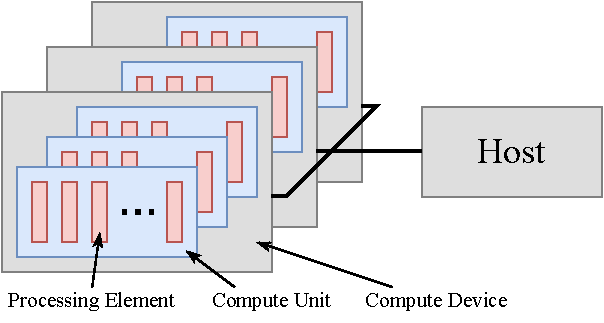
\includegraphics[width=\linewidth]{opencl/architecture}
    \caption{Архитектура OpenCL}
    \label{OpenCLArchitecture:image}
\end{figure}

Физически \textit{computer unit} представляет собой \textit{work-group}, который состоит из ячеек \textit{work-item} (элементов работы), которые и выполняют вычисления (рисунок~\ref{OpenCLWorkGroup:image}).

Команды в OpenCL образуют очередь. \textit{Host} направляет команды на устройства. Эти команды становятся в очередь аналогичных команд. Можно реализовать очередь с соблюдением порядка и без соблюдения.
Функции работы с получением ID \textit{work-group} и \textit{work-item} приведены на рисунке~\ref{OpenCLWorkGroupItemExample:image}.

\textbf{Виды памяти в OpenCL-устройствах.} Для взаимодействия с данными программист может использовать разные уровни памяти. На рисунке~\ref{OpenCLMemory:image} видно, что существуют следующие виды памяти:

\begin{itemize}
    \itemЧастная память (private). Самая быстрая из всех видов. Эксклюзивна для каждого элемента работы~\cite{Bastrakov2011}.
    \itemЛокальная память (local memory). Может быть использована компилятором при большом числе локальных переменных в какой-либо функции. По скоростным характеристикам локальная память значительно медленнее, чем регистровая. Доступ из всех элементов работы внутри одной work-group.
    \itemКонстантная память (constant memory). Достаточно быстрая из доступных GPU. Есть возможность записи данных с хоста, но при этом в пределах всего GPU возможно лишь чтение. Динамическое выделение, в отличие от глобальной памяти, в константной не поддерживается.
    \itemГлобальная память (global memory). Самый медленный тип памяти, из доступных GPU. Глобальные переменные можно выделить с помощью спецификатора, а также динамически. Глобальная память в основном служит для хранения больших объемов данных, поступивших на device с host’а. В алгоритмах, требующих высокой производительности, число операций с глобальной памятью необходимо свести к минимуму.
\end{itemize}	

\begin{figure}[H]
    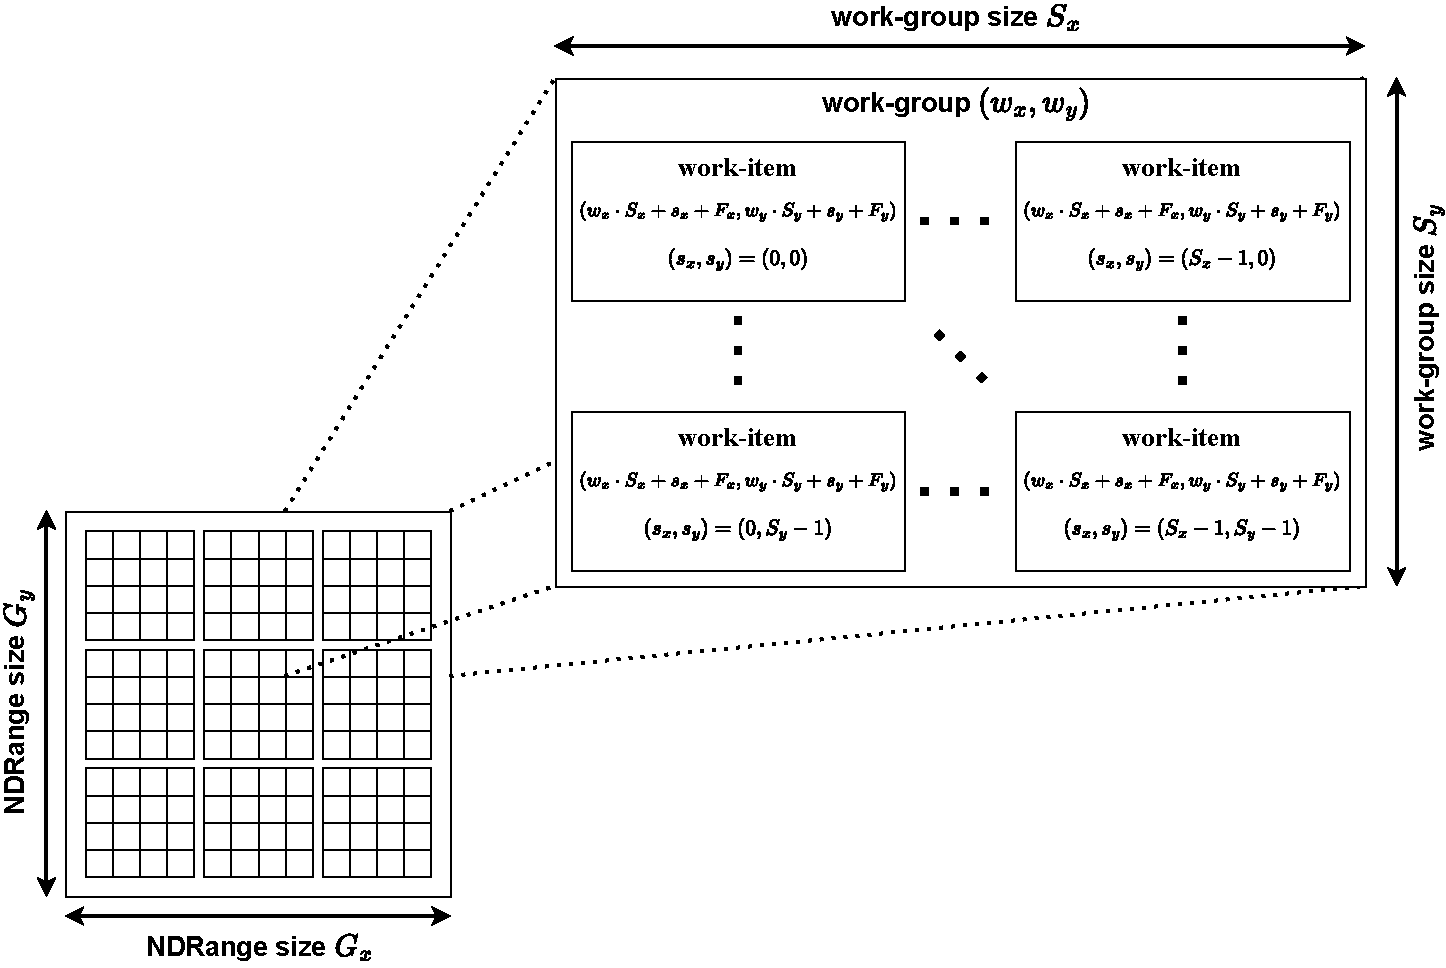
\includegraphics[width=\linewidth]{opencl/work-group}
    \caption{Архитектура OpenCL -- строение work-group элемента}
    \label{OpenCLWorkGroup:image}
\end{figure}

\begin{figure}[H]
    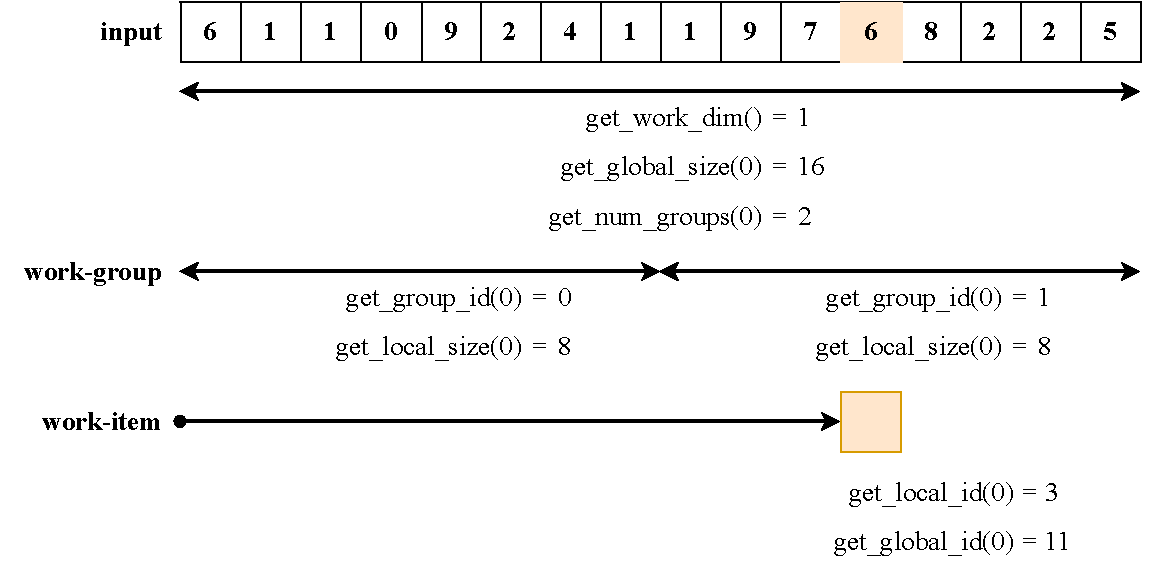
\includegraphics[width=\linewidth]{opencl/work-group-item}
    \caption{OpenCL. Работа с work-group и work-item}
    \label{OpenCLWorkGroupItemExample:image}
\end{figure}

\begin{figure}[H]
    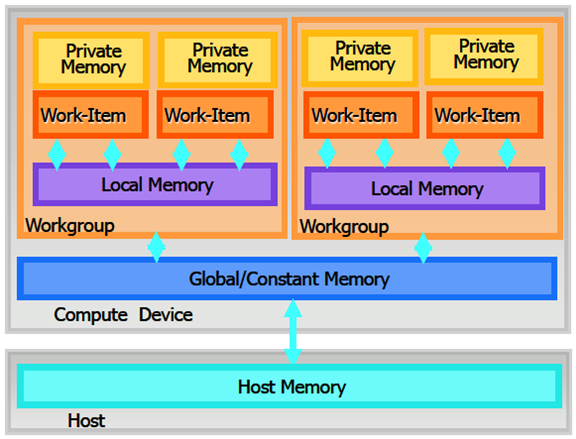
\includegraphics[width=\linewidth]{opencl/memory}
    \caption{Виды памяти в OpenCL-устройствах}
    \label{OpenCLMemory:image}
\end{figure}

Программист должен явным образом управлять и контролировать копирования между разными видами памяти.

Программа на OpenCL может включать в себя следующую последовательность действий:
    \begin{enumerate}
        \item\textbf{Выбор платформы:} clGetPlatformIDs, clGetPlatformInfo
        \item\textbf{Выбор устройства:} clGetDeviceIDs, clGetDeviceInfo
        \item\textbf{Создание вычислительного контекста:} cl\-Create\-Context\-From\-Type
        \item\textbf{Создание очереди команд:} cl\-Create\-Command\-Queue\-With\-Pro\-per\-ties
        \item\textbf{Выделение памяти в виде буферов:} clCreateBuffer
        \item\textbf{Создание объекта <<программа>>:} clCreateProgramWithSource
        \item\textbf{Компиляция кода:} clBuildProgram
        \item\textbf{Создание <<ядра>> (объект kernel):} clCreateKernel
        \item\textbf{Работа c Work-Group:} clGetKernelWorkGroupInfo 
        \item\textbf{Выполнение ядра:} clEnqueueNDRangeKernel 
        \item\textbf{Ожидание выполнения ядра:} clWaitForEvents 
        \item\textbf{Profiling:} clGetEventProfilingInfo
    \end{enumerate}

Далее рассмотрим некоторые из этих действий подробнее.

\textbf{Выбор платформы, устройства и создание контекста.} Контекст \textit{(context)} служит для управления объектами и ресурсами OpenCL. Все ресурсы OpenCL привязаны к контексту. С контекстом ассоциированы следующие данные (рисунок~\ref{OpenCLContext:image}):

\begin{itemize}
    \itemустройства
    \itemобъекты программ
    \itemядра
    \itemобъекты памяти
    \itemочереди команд~\cite{Bastrakov2011}.
\end{itemize}

\begin{figure}[H]
    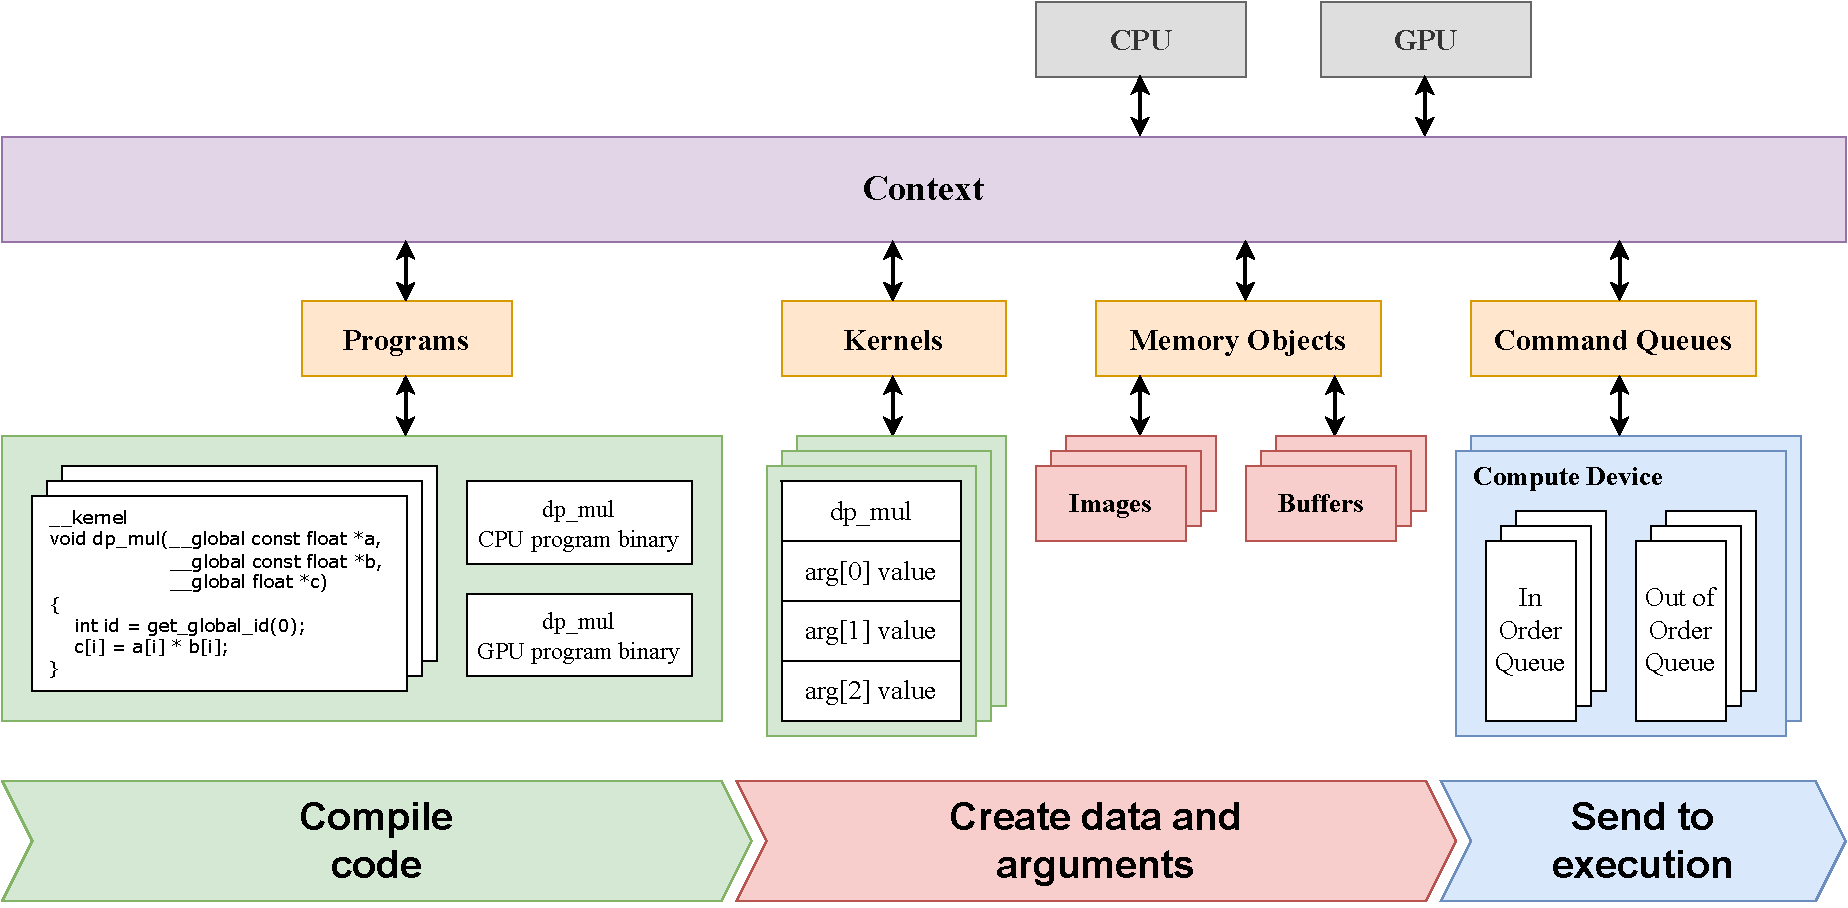
\includegraphics[width=\linewidth]{opencl/context}
    \caption{Архитектура OpenCL -- контекст}
    \label{OpenCLContext:image}
\end{figure}

Можно получить информацию о платформе и вычислительных ядрах с помощью специальных функций, чтобы затем создать контекст:

\begin{itemize}
    \item\code{clGetPlatformInfo()} -- содержит информацию о платформе, на которой работает программа
    \item\code{clGetDeviceDs()} -- содержит информацию о подключенных устройствах
    \item\code{clGetDeviceInfo()} -- содержит информацию о данном девайсе: его тип, совместимость и тд.
\end{itemize}

Контекст можно создать при помощи функции \code{clCreateContext()}. Вот пример его создания:

\inputminted{c++}{listings/OpenCLContextExample.c}

В строку 3 мы получаем ID платформы, в строке 7 ID первого GPU на этой платформе, в строке 11 создаем контекст для этого девайса. Подробнее про аргументы, принимаемые этими функциями, можно прочитать в документации. Есть также функция \code{clCreateContextFromType()} для создания контекста, ассоциированного с устройствами определенного типа.

\textbf{Ядро.} Ядром называется функция, являющаяся частью программы и параллельно исполняющаяся на устройстве. Ядро является аналогом потоковой функции. Часть, выполняющаяся на устройстве, состоит из набора ядер, объявленных с квалификатором \textbf{\_kernel}. Компилирование ядер может осуществляться во время исполнения программы с помощью функций API~\cite{Bastrakov2011}. Работа в рамках одной work group выполняется одновременно всеми work items.

При написании ядра можно использовать следующие квалификаторы для переменнных~\cite{GorshkovBastrakov2012}:

\begin{itemize}
    \item\_\_global или global -- данные в глобальной памяти.
    \item\_\_constant или constant -- данные в константной памяти.
    \item\_\_local или local -- данные в локальной памяти.
    \item\_\_private или private -- данные в частной памяти.
    \item\_\_read\_only и \_\_write\_only -- квалификаторы режима доступа.
\end{itemize}

\sloppy
Скомпилировать код ядра можно с помощью функций \code{clCreateProgramWithSource()}, \code{clBuildProgram()} и \code{clCreateKernel()}. Пример компиляции и запуска программы по перемножению двух массивов приведен в листинге ниже.

\inputminted{c++}{listings/opencl_kernel_example.cpp}

В результате обычная программа, ранее написанная на языке Си, превратится в программу, написанную для ядра. Листинг обоих программ приведен далее.

\noindent
\begin{minipage}[t]{.5\textwidth}
    \begin{minted}{c++}
    void trad_mul(int n, 
                  const float *a, 
                  const float *b, 
                  float *c) {
        int i;
        for (i = 0; i < n; ++i)
            c[i] = a[i] * b[i];
    }
    \end{minted}
\end{minipage}%
\begin{minipage}[t]{.5\textwidth}
    \begin{minted}{c++}
    __kernel 
    void dp_mul(__global const float *a, 
                __global const float *b, 
                __global float *c) {

        int id = get_global_id(0);
        c[i] = a[i] * b[i];
    } // execute over n "work items"
    \end{minted}
\end{minipage}

\bigskip

Подробнее об остальных особенностях технологии OpenCL можно прочитать в источнике~\cite{Bastrakov2011} %на ресурсе \url{http://docplayer.ru/37490743-Programmirovanie-na-opencl.html} 
и в официальной документации:

\begin{enumerate}
    \item OpenCL -- официальный сайт:\url{http://www.khronos.org/opencl}
    \item Intel OpenCL: \url{http://software.intel.com/en-us/articles/intel-opencl-sdk}
    \item NVIDIA OpenCL: \url{http://www.nvidia.ru/object/cuda_opencl_new_ru.html}
    \item NVIDIA OpenCL: \url{https://developer.nvidia.com/opencl}
    \item AMD OpenCL: \url{http://www.amd.com/us/products/technologies/stream-technology/opencl/Pages/opencl.aspx}
\end{enumerate}

\subsection{Архитектура CUDA}
\label{CUDA:section}
CUDA -- архитектура параллельных вычислений на графических процессорах NVIDIA. Технология была представлена компанией в 2006 году. Подразумевалось, что новые компоненты снимут существующие тогда ограничения, а именно -- позволят использовать GPU для операций общего назначения, в том числе для вычислений с плавающей точкой. Но технология не сразу общедоступной, так как программистам все еще приходилось маскировать вычисления под графические задачи. Для разрешения проблемы NVIDIA на базе языка С создала новый язык -- CUDA C, в котором появились ключевые слова, позволяющие управлять устройствами~\cite{KandrotSanders2022}.

\subsubsection*{Общие понятия, сборка и запуск приложения} 
CUDA включает в себя расширение языка С (с элементами С++), набор оптимизированных библиотек, специальные драйверы CUDA. Позволяет увеличивать производительность вычислений благодаря использованию графических процессоров фирмы Nvidia.
Для разработки могут использоваться все основные операционные системы (Windows, Linux, MacOS).
При этом для написания программ возможно использование различных языков программирования. Первым был использован язык CUDA C - расширение языков С/C++, также можно использовать технологии OpenCL и DirectCompute. Кроме того, есть сторонние реализации для Java, Python, C\#.
Для разработки на CUDA необходимы следующие её составляющие:
\begin{itemize}
    \item\textbf{CUDA Driver} -- драйвер, обеспечивающий выполнение скомпилированных приложений на CUDA;
    \item\textbf{Cuda Toolkit} -- инструмент для разработки приложений, включающий в себя~\cite{Gergel2016}:
    \begin{itemize}
        \item Компилятор CUDA C NVCC (NVIDIA C Compiler);
        \item Оптимизированные библиотеки для графического процессора;
        \item Профилировщик;
        \item Драйвер CUDA Runtime;
        \item Документация.
    \end{itemize}
    \item\textbf{GPU Computing SDK} -- включает в себя некоторое количество примеров приложений для CUDA для базовых сценариев использования.
\end{itemize}

\subsubsection*{Преимущества CUDA}
\begin{itemize}
    \item Интерфейс основан на стандартном языке программирования C с некоторыми ограничениями, что упрощает изучение данной технологии;
    \item Более эффективные пересылки между памятью CPU и видеопамять;
    \item Полная поддержка целочисленных и побитовых операций;
    \item Разделяемая между потоками память (shared memory) размером в 16 Кб может быть использована под организованный пользователем кэш с более широкой полосой пропускания, чем при выборке из обычных текстур.
\end{itemize}

\subsubsection*{Ограничения CUDA}
\begin{itemize}
    \item Все функции, выполняемые на устройстве, не поддерживают рекурсии (в версии CUDA Toolkit 3.1 поддерживает указатели и рекурсию) и имеют некоторые другие ограничения;
    \item Неточные вычисления при работе с числами с плавающей запятой.
\end{itemize}

\subsubsection*{Программная модель CUDA} 
При создании программы CPU будет являться хостом (host), а GPU-ядром (kernel).

Рассмотрим внутреннюю программную модель CUDA, а также пример создания kernel-функции, исполняемой на устройстве.

\begin{figure}[H]
    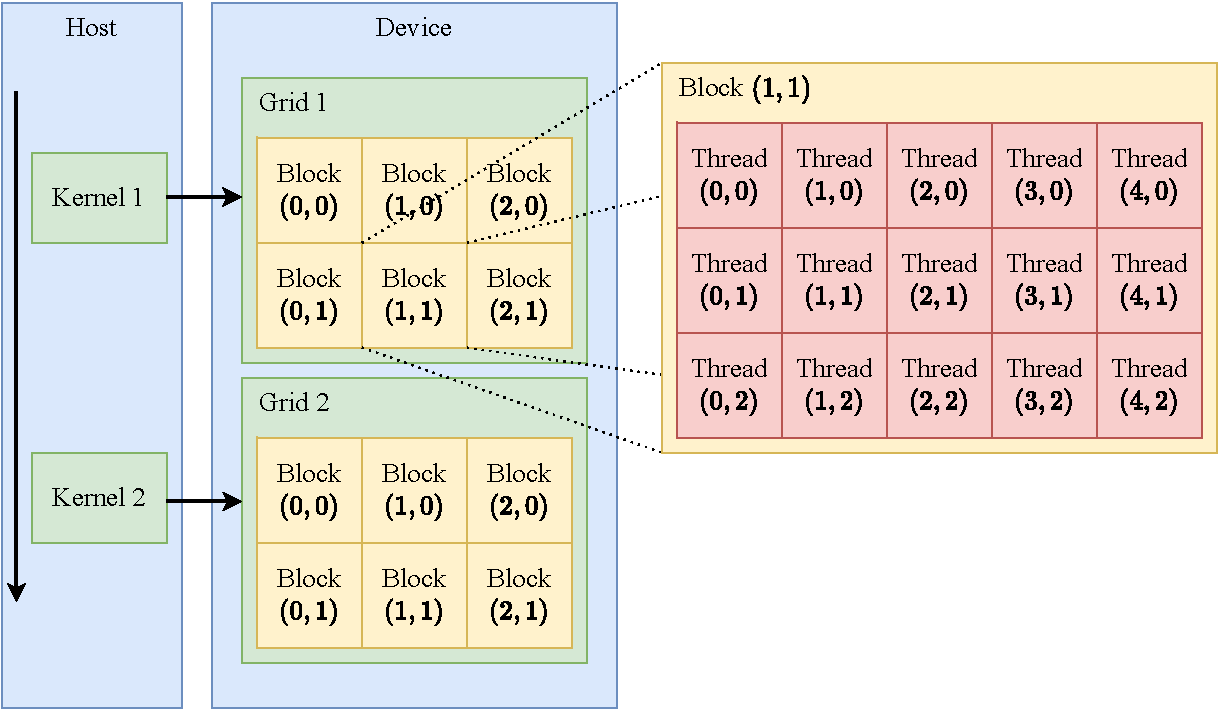
\includegraphics[width=\linewidth]{cuda/architecture}
    \caption{Архитектура CUDA}
    \label{CUDAArchitecture:image}
\end{figure}

Технология CUDA позволяет определять специальные функции – ядра (kernels), которые выполняются параллельно на ГПУ в виде множества различных потоков (threads). Таким образом, ядро является аналогом потоковой функции. Каждый поток исполняется на одном CUDA-ядре, используя собственный стек инструкций и локальную память. Отдельные потоки группируются в блоки потоков (thread block) одинакового размера, при этом каждый блок потоков выполняется на отдельном мультипроцессоре.
На аппаратном уровне потоки блока группируются в так называемые варпы (warps) по 32 элемента (на всех текущих устройствах), внутри которых все потоки параллельно выполняют одинаковые инструкции (по принципу SIMD\footnote{SIMD -- Single Instruction, Multiple Data}).
В свою очередь, блоки потоков объединяются в решетки блоков потоков (grid of thread blocks). Взаимодействие потоков из разных блоков во время работы ядра затруднено: отсутствуют явные инструкции синхронизации, взаимодействие возможно через глобальную память и использованием атомарных функций (другим вариантом является разбиение ядра на несколько ядер без внутреннего взаимодействия между потоками разных блоков).
Каждый поток внутри блока потоков имеет свои координаты (одно-, двух- или трехмерные), которые доступны через встроенную переменную \texttt{threadIdx}. В свою очередь, координаты блока потоков (одно-, двух- или трехмерные) внутри решетки определяются встроенной переменной \v{blockIdx}. Данные встроенные переменные являются структурами с полями \texttt{.x}, \texttt{.y}, \texttt{.z}~\cite{DenisenkoSatanin2012}.

Встроенные переменные-векторы:
\begin{itemize}
    \item\code[text]{uint3 threadIdx} -- индекс нити в блоке
    \item\code[text]{dim3 blockDim} -- размеры блока
    \item\code[text]{uint3 blockIdx} -- индекс блока в сетке
    \item\code[text]{dim3 gridDim} -- размеры сетки
\end{itemize}

\noindentЛинейный индекс потока (одномерный случай): 
\mint{cuda}{int tid = blockIdx.x * blockDim.x + threadIdx.x;}

\noindentОбщее число потоков (одном. случай): 
\mint{cuda}{int threads_total = blockDim.x * gridDim.x;}

\textbf{Kernel-функция.} Пример создания функции и вызов ее с device:
\begin{minted}{cuda}
__global__ void kernel_function(float* data) { ... }

kernel_function<<<blocks, threads, nshared, stream>>> (data);
\end{minted}

Используемые параметры:
\begin{itemize}
    \item\texttt{blocks (grid)} -- задает число блоков
    \item\texttt{threads (block)} -- задает число нитей в блоке
    \item\texttt{nshared} -- количество дополнительной shared-памяти, выделяемое блоку \textit{(необязательный параметр)}
    \item\texttt{stream} -- номер потока CUDA, в котором нужно запустить ядро \textit{(необязательный параметр)}
\end{itemize}

Создаётся \texttt{blocks * threads} вычислительных нитей в процессе выполнения функции.

\textbf{Определение размера параметров.} Оба параметра представляют собой вектор из трёх координат. В CUDA есть функция, с помощью которой можно вычислить размер блоков, а также формула для размера грида.

\noindentФункция для определения подходящего blockSize:
\mint{cuda}{cudaOccupancyMaxPotentialBlockSize(&minGridSize, func_name, 0, N);}

\noindentФормула для gridSize:
\mint{cuda}{gridSize = (N + blockSize - 1) / blockSize;}

\textbf{Используемые идентификаторы.} Для определения памяти используется три идентификатора - device, global и host.

Область с пометкой device выполняется на устройстве, вызываться может также только там. Область с пометкой global, с которой обычно и создаются функции, можно вызвать откуда угодно, а выполняться будет всё на устройстве. И по умолчанию всегда ставится host, который выполняется на CPU и вызывается оттуда же.

\begin{table}[H]
    \centering
    \begin{tabular}{|c|c|c|}
    \hline
    \thead{Идентификатор} & \thead{Можно вызвать с}   & \thead{Выполняется на}     \\ \hline
    \texttt{\_\_device\_\_}  & device            & device         \\ \hline
    \texttt{\_\_global\_\_}  & host, device      & device         \\ \hline
    \texttt{\_\_host\_\_}    & host              & host           \\ \hline
    \end{tabular}
\end{table}

Для переменных также есть device. Кроме него есть ещё constant для констант и shared для общей памяти между блоками.

\begin{table}[H]
    \centering
    \begin{tabular}{|c|c|c|}
    \hline
    \thead{Идентификатор} & \thead{Расположение в памяти} & \thead{Область видимости} \\ \hline
    \texttt{\_\_device\_\_}      & device (global)       & сетка \\ \hline
    \texttt{\_\_constant\_\_}    & device (constant)     & сетка \\ \hline
    \texttt{\_\_shared\_\_}      & device (shared)       & блок  \\ \hline
    \end{tabular}
\end{table}

\subsubsection*{Структура памяти CUDA}
Виды памяти в CUDA:
\begin{itemize}
    \item Локальная (local)
    \item Разделяемая (shared)
    \item Глобальная (global)
    \item Память констант (constant)
    \item Текстурная (texture)
\end{itemize}

Каждый поток обладает своей локальной памятью (local memory).
Все потоки внутри блока имеют доступ к быстрой разделяемой памяти блока (shared memory), время жизни которой совпадает со временем жизни блока. Разделяемая память блока разбита на страницы, при этом доступ к данным на разных страницах осуществляется параллельно.

Все потоки во всех блоках имеют доступ к глобальной памяти устройства (global memory или device memory), которая всегда хранит своё состояние во время работы программы.

Всем потокам также доступны два вида общей кэшируемой памяти для чтения: константная (constant) и текстурная (texture). Так же как и в глобальной памяти устройства, данные хранятся всегда во время работы программы. При этом текстурная память обеспечивает различные режимы адресации и поддерживает фильтрацию для определенных форматов данных. Фильтрация реализована на аппаратном уровне и может эффективно использоваться в различных задачах~\cite{Gergel2016}.

\begin{figure}[H]
    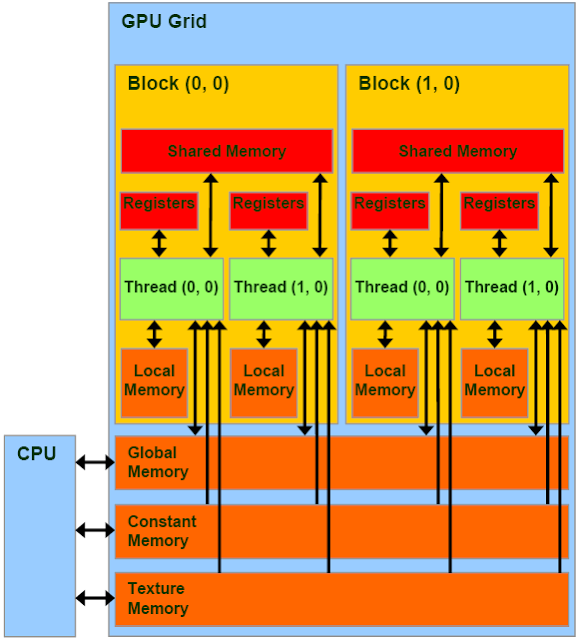
\includegraphics[width=\linewidth]{cuda/memory}
    \caption{CUDA. Структура памяти}
    \label{CudaMemory:image}
\end{figure}

\subsubsection*{Основные функции CUDA для работы с памятью}
В CUDA основными функциями являются функции для выделения и очистки памяти, а также пересылка данных между устройствами.
\begin{itemize}
    \item\texttt{cudaError\_t cudaMalloc(void **devPtr, size\_t size)} -- поз\-во\-ля\-ет выделить память на GPU размером \texttt{size} с указателем на \texttt{devPtr}. Возвращает код из структуры \texttt{cudaError\_t}, в котором будет код успеха или один из многочисленных кодов ошибок с описанием.
    \item\texttt{cudaError\_t cudaFree(void *devPtr)} -- позволяет очистить область памяти, на которую указывает \texttt{devPtr}. Возвращает код из структуры \texttt{cudaError\_t}, в котором будет код успеха или один из многочисленных кодов ошибок с описанием.
    \item\texttt{cudaError\_t cudaMemcpy(void *dst, const void *src, \\ size\_t size, enum cudaMemcpyKind kind)} -- позволяет скопировать данные размера size с источника \texttt{src} на получателя \texttt{dst}. Возвращает код из структуры \texttt{cudaError\_t}, в котором будет код успеха или один из многочисленных кодов ошибок с описанием. Последний параметр \texttt{kind} показывает, куда и откуда необходимо отправить данные, принимает следующие значения:
    \begin{itemize}
        \item \texttt{cudaMemcpyHostToHost} -- копирование с CPU на CPU
        \item \texttt{cudaMemcpyHostToDevice} -- копирование с CPU на GPU
        \item \texttt{cudaMemcpyDeviceToHost} -- копирование с GPU на CPU
        \item \texttt{cudaMemcpyDeviceToDevice} -- копирование с GPU на GPU
        \item \texttt{cudaMemcpyDefault} -- позволяет не указывать направление, поскольку оно может быть вычислено по принадлежности указателей.
    \end{itemize}
\end{itemize}

\subsubsection*{Синхронизация событий}
Для каждой многопоточной программы необходима синхронизация потоков перед выполнением каких-либо нераспараллеленных действий или при доступе к общему ресурсу. В CUDA есть возможность синхронизации потоков с использованием cuda-event, которое работает аналогично барьерам.

Необходимо создать и записать события, а потом вызывать функцию синхронизации в нужном месте программы, где все потоки будут ожидать завершения остальных. Также в конце программы необходимо удалить данное событие.

Используемые функции:
\begin{itemize}
    \item \texttt{cudaEvent\_t syncEvent} -- создание переменной для events;
    \item \texttt{cudaEventCreate(\&syncEvent)} -- создание и инициализация \linebreak event;
    \item \texttt{cudaEventRecord(syncEvent, nullptr)} -- запись этого события барьера, чтобы все потоки о нём узнали;
    \item \texttt{cudaEventSynchronize(syncEvent)} -- метка синхронизации, то есть место, где потоки должны ожидать выполнения друг друга;
    \item \texttt{cudaEventDestroy(syncEvent)} -- удаление event.
\end{itemize}

Описанный выше пример подходит для синхронизации на host. Но также есть функции, которые можно вызывать на самом устройстве~\cite{CudaSyncHabr}:
\begin{itemize}
    \item\texttt{\_\_syncthreads()} -- функция заставит каждый поток ждать, пока все остальные потоки этого блока достигнут этой точки и все операции по доступу к разделяемой и глобальной памяти, совершенные потоками этого блока, завершатся и станут видны потокам этого блока.
    \item\texttt{\_\_threadfence\_block()} -- будет заставлять ждать вызвавший её поток, пока все совершенные операции доступа к разделяемой и глобальной памяти завершатся и станут видны потокам этого блока.
    \item\texttt{\_\_threadfence()} -- будет заставлять ждать вызвавший её поток, пока все совершенные операции доступа к разделяемой памяти станут видны потокам этого блока, а операции с глобальной памятью — всем потокам на графическом устройстве.
    \item\texttt{\_\_threadfence\_system()} -- подобна \texttt{\_\_threadfence()}, но включает синхронизацию с потоками на CPU, при использовании весьма удобной page-locked памяти.
\end{itemize}

\subsubsection*{Управление устройствами}
В CUDA представлен простой интерфейс, позволяющий узнать, какие устройства с какими параметрами есть в системе. Примерами таких функций служат:
\begin{itemize}
    \sloppy
    \item\texttt{cudaError\_t cudaGetDeviceCount(int *count)} -- получение числа доступных устройств;
    \item\texttt{cudaError\_t cudaGetDevice(int *dev)} -- получение номера текущего используемого устройства;
    \item\texttt{cudaError\_t cudaGetDeviceProperties(struct cudaDeviceProp *prop, int dev)} -- заполнение структуры, содержащей свойства устройства;
    \item\texttt{cudaError\_t cudaChooseDevice(int *dev, const struct cudaDeviceProp *prop)} -- выбор устройства, которое лучше всего соответствует переданной конфигурации;
    \item\texttt{cudaError\_t cudaSetDevice(int dev)} -- установка определённого устройства.
\end{itemize}

Сначала полезно узнать, сколько всего устройств при помощи функции \texttt{cudaGetDeviceCount}:
\begin{minted}{cuda}
int count;
cudaDeviceProp prop; 
cudaGetDeviceCount(&count);
\end{minted}

Далее итеративно можно прочитать параметры каждого устройства:
\begin{minted}{cuda}
for (int i=0; i<count; ++i)
    cudaGetDeviceProperties(&prop, i);
\end{minted}

С полным списком параметров в структуре \code{cudaDeviceProp} можно ознакомится в документации~\cite{CudaDeviceProp}.
% \url{https://docs.nvidia.com/cuda/cuda-runtime-api/structcudaDeviceProp.html}.

\subsubsection*{Обработка ошибок}
Каждая CUDA-функция возвращают структуру \code[cuda]{cudaError_t}, за счёт которой можно понять, успешно ли произошло, например, выделение памяти. Примеры кодов возврата:
\begin{itemize}
    \item\code[cuda]{cudaSuccess} -- при успешном завершении
    \item\code[cuda]{cudaErrorInvalidValue} -- неправильно переданный аргумент при вызове CUDA-функции
    \item\code[cuda]{cudaErrorMemoryAllocation} -- ошибка выделения памяти
    \item\code[cuda]{cudaErrorInitializationError} -- невозможно вызвать функцию, поскольку CUDA driver не проинициализирован
\end{itemize}

Кроме того, есть функция для получения последней брошенной ошибки для её последующей обработки в нужном месте программы (также возвращает код ошибки из \code[cuda]{cudaError_t}).

\mint{cuda}{cudaError_t error = cudaGetLastError();}

\subsubsection*{Пример программы}
\begin{minted}{cuda}
__global__ void proccess_smth(double* arr, int size) { 
    // calculating something
}

int main(int argc, char *argv[]) {
    // prepare array arr by host
    // allocate bytes on device
    size_t arr_size = sizeof(double) * N;
    cudaMalloc(&arr_gpu, v);
    
    // copy to device
    cudaMemcpy(arr_gpu, arr, arr_size, cudaMemcpyHostToDevice);
    proccess_smth<<<gridSize, blockSize>>>(arr_gpu, N);()
    
    // copy result to host
    cudaMemcpy(arr, arr_gpu, arr_size, cudaMemcpyDeviceToHost); 
    cudaFree(arr_gpu) ;
    ...
}
\end{minted}

При использовании синхронизации код преобразуется следующим образом:
\begin{minted}{cuda}
int main(int argc, char *argv[]) {
    // define event to synchronize host & device 
    cudaEvent_t syncEvent;
    cudaEventCreate(&syncEvent); 
    cudaEventRecord(syncEvent, nullptr);
    
    proccess_smth<<<gridSize, blockSize>>>(arr_gpu, N);()
    
    cudaEventSynchronize(syncEvent);
    ... 
}
\end{minted}

\subsubsection*{Профилирование}
Вместе с CUDA обычно поставляется также отдельный профилировщик. NVVP\footnote{NVIDIA Visual Profiler} -- визуальная составляющая базового профилировщика. Пример интерфейса основного окна представлен на рисунке~\ref{CudaProfiling:image}.

\begin{figure}[H]
    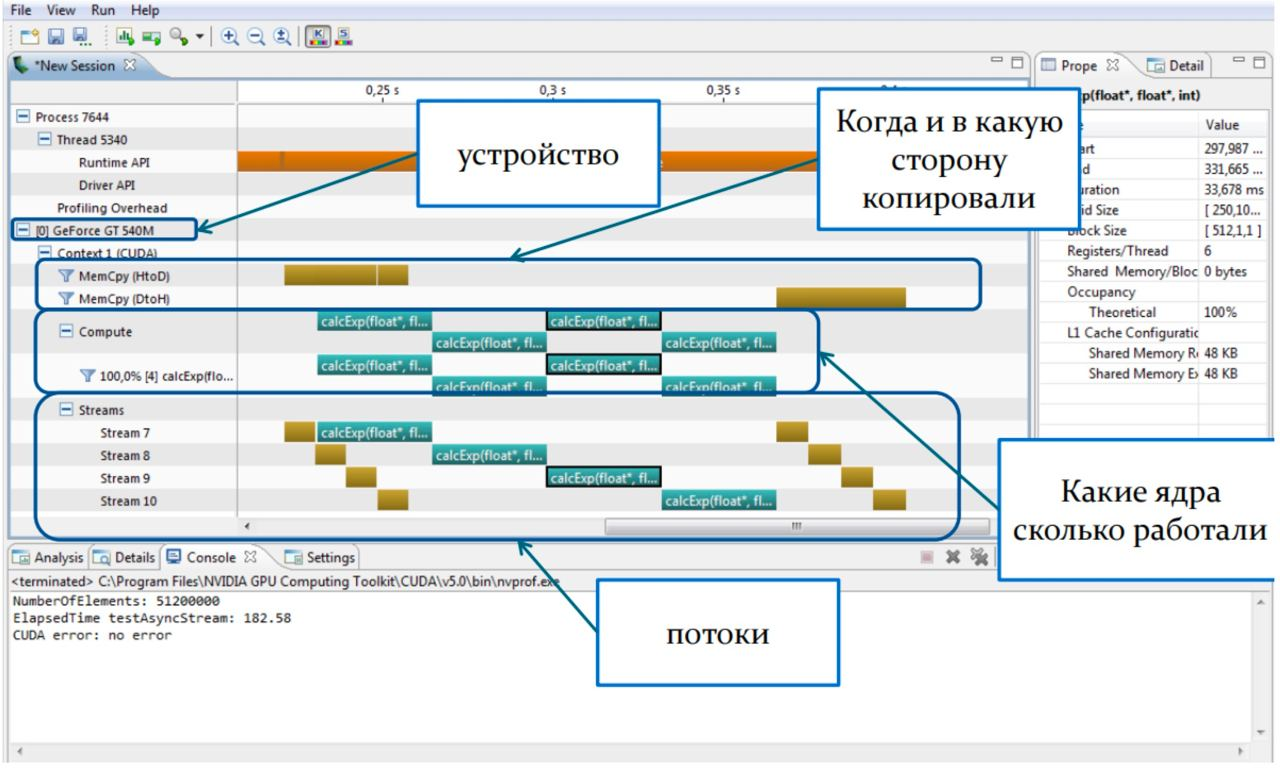
\includegraphics[width=\linewidth]{cuda/profiling_app}
    \caption{Пример интерфейса профилировщика CUDA}
    \label{CudaProfiling:image}
\end{figure}

\noindentКоманда для профилирования:
\mint{text}{nvprof [options] [application] [application-arguments]}

\noindentПример команды:
\mint{text}{nvprof --unified-memory-profiling per-process-device ./program}

\noindentПример вывода~\cite{Rutsh2011}: \\
\noindent\resizebox{\textwidth}{!}{
    \begin{tabular}{|rrrrrrl|}
        \hline
        \multicolumn{7}{|l|}{==5286== NVPROF is profiling process 5286, command: ./program [args]} \\
        \multicolumn{7}{|l|}{==5286== Profiling application: ./program [args]} \\
        \multicolumn{7}{|l|}{==5286== Profiling result:} \\
        \textbf{Time(\%)} & \textbf{Time} & \textbf{Calls} & \textbf{Avg} & \textbf{Min} & \textbf{Max} & \textbf{Name} \\
        26.47\% & 639.68us & 100 & 6.41us & 6.01us & 16.2us & func1(double*, double*, int) \\
        22.99\% & 555.58us & 100 & 5.55us & 5.50us & 7.13us & func2(double*, int) \\
        18.48\% & 446.68us & 300 & 1.49us & 1.21us & 9.08us & [CUDA memcpy HtoD] \\
        16.27\% & 393.29us & 100 & 3.93us & 3.65us & 12.1us & func3(double const *, double*, int) \\
        15.78\% & 381.40us & 300 & 1.27us & 1.09us & 2.43us & [CUDA memcpy DtoH] \\
        \hline
    \end{tabular}
}

\texttt{{\textendash\textendash}unified-memory-profiling per-process-device} -- общее потребление памяти и время выполнения вызываемых функций. per-process-device расписывает для каждого процесса.

Также в выводе можно увидеть общее, минимальное, максимальное и среднее (суммарное) время работы для каждой функции устройства, а также затраты на копирование данных с CPU на GPU и обратно.

\texttt{{\textendash\textendash}print-gpu-trace} -- печатать более детальную информацию по каждому запуску kernel и отсортировать в хронологическом порядке.

\subsubsection*{Сравнение CUDA и OpenCL}
Достоинство OpenСL -- открытый стандарт, программы будут работать на любом устройстве поддерживающем этот стандарт, в том числе на CPU. С другой стороны, исходные программы, использующие OpenCL, состоят из двух экземпляров: основная программа (для CPU) и текст для OpenCL. Соответственно, при внесении изменений всегда требуется поддерживать актуальными оба экземпляра. CUDA с этой точки зрения -- полная противоположность OpenCL, так как, с одной стороны, выполняется только на GPU от NVIDIA, с другой стороны, ограничивается наличием единого исходного текста -- файла с расширением .cu.

Программа, использующая OpenCL, может быть запущена на ряде слабосвязанных устройств, хотя потребуются дополнительные усилия, чтобы реализовать программу таким образом, чтобы минимизировать привязку к конкретному устройству. Ядро OpenCL может быть скомпилировано во время выполнения, хотя это отрицательно скажется на скорости. CUDA, в силу того, что разрабатывается той же компанией, что и аппаратное обеспечение может представить лучшую производительность, но в общем случае это зависит от качества кода, выполняемой задачи и используемых алгоритмов.

CUDA -- проприетарный фреймворк NVIDIA, в то время как у OpenCL окрыт исходный код. Хотя комьюнити CUDA больше, она чаще обсуждается на форумах, обладает большей документацией и считается более простой для понимания и изучения. Тем не менее комьюнити OpenCL растет с каждым годом.

OpenCL будет работать на любой ОС, в то время как CUDA будет работать только на ведущих ОС, с условием использования NVIDIA.

Для CUDA существуют много высокопроизводительных библиотек, для OpenCL их меньше~\cite{Krasnov2002}.

\subsubsection*{Сферы применения CUDA}
\textbf{Обработка медицинских изображений.} В данной сфере есть несколько проблем. При проведении исследований (УЗИ, МРТ и др.) необходимо быстро получать, обрабатывать и сохранять большие объемы данных. Сложность в том, что использовать сжатие крайне нежелательно. Раньше подобные исследования были слишком дорогими для клинического исследования, а следовательно, страдали люди, которые пропустили первые стадии серьезных заболеваний. CUDA позволила разрешить проблему быстрой обработки больших объемов информации, что сделало исследования более доступными. Это, в свою очередь, положительно сказалось на постановке диагнозов и лечении пациентов с онкологическими заболеваниями.

\textbf{Вычислительная гидродинамика.} Для проектирования эффективных винтов и лопаток необходимо проведение экспериментов со сложными численными моделями, так как требуется анализ сложного движения воздуха и жидкости, обтекающих винты и лопатки. CUDA сделала подобные исследования более доступными, сегодня частичные результаты доступны уже через несколько секунд.

\textbf{Окружающая среда.} Проблема возникла из-за поверхностно-активных веществ (ПАВ) чистящих сре\-дств, которые отвечают за эффективность средства. ПАВ хорошо сцепляется с частицами грязи, а также с частицами воды. Проблема в том, что эффективность часто сопровождается пагубным воздействием на окружающую среду. Поэтому требуется проведение экспериментов по варьированию комбинаций компонентов и загрязнений, чтобы опередить наиболее эффективный и наименее вредный состав. Данная задача может быть разрешена с использованием CUDA.
\subsection{Ошибки в многопоточных приложениях}

Помимо привычных для программиста ошибок, встречающихся в компьютерных программах, существует ряд ошибок, специфичных для параллельного программирования. Эти ошибки обусловлены следующими особенностями параллельных программ:

\begin{itemize}
    \item\textbf{Синхронизация потоков.} Программист должен обеспечить корректную последовательность выполняемых разными потоками операций. В общем случае невозможно точно сказать, в какой последовательности будут выполняться команды потоков, т.к. операционная система может в произвольный момент времени приостановить выполнение потока.
    \item\textbf{Взаимодействие потоков.} Также программист не должен допускать конфликтов при обращении к общим для потоков областям памяти. 
    \item\textbf{Балансировка нагрузки.} Если в распараллеленной программе один из потоков выполняет 99\% работы, то даже на 64-ядерной системе параллельное ускорение едва ли превысит значение 1.01.
    \item\textbf{Масштабируемость.} В идеале параллельная программа должна одинаково хорошо распараллеливать выполняемую работу на любом доступном числе процессоров. Однако добиться этого нелегко, и это часто приводит к трудно обнаруживаемым ошибкам.
\end{itemize}

Рассмотрим далее подробнее следующий неполный перечень типовых ошибок, возникающих в параллельных программах независимо от используемой технологии распараллеливания:

\begin{itemize}
    \itemПотеря точности операций с плавающей точкой.
    \itemВзаимные блокировки (deadlock).
    \itemСостояния гонки (race conditions). 
    \itemПроблема АВА.
    \itemИнверсия приоритетов.
    \itemГолодание (starvation).
    \item False Sharing.
\end{itemize}

\textbf{Потеря точности.} Если параллельная программа используется для проведения операций с плавающей точкой при работе с вещественными переменными, расположенными в общей для потоков памяти, то при каждом запуске программы может получаться разный результат вещественных расчётов. Это объясняется тем, что при работе нескольких потоков невозможно точно предсказать, в каком порядке операционная система предоставит этим потокам процессор, т.к. в любой момент любой поток может быть временно приостановлен по усмотрению ОС. В свою очередь, это приводит к неопределённой последовательности выполнения операций с плавающей точкой, результат которых, как известно, может зависеть от порядка.

Рассмотрим пример, иллюстрирующий сказанное:

\begin{minted}{c++}
int i;
float s = 0;

#pragma omp parallel for reduction(+:s) num_threads(8)
for (i = 1; i < 1000000; ++i)
    s += 1.0 / i;

printf("s=%f\n", s);
\end{minted}

% \inputminted{c++}{listings/OpenMPExample16.cpp}

Здесь в переменную s суммируются результаты вещественных вычислений восемью потоками. В результат получается s=14.393189. Однако если эту же программу выполняет всего один поток (для этого нужно в строке 3 установить значение параметра num\_threads в 1), то результат получится иным: s=14.357357. Различие между двумя приведёнными значениями составляет примерно 0.25\%. 

Получается, что параллельная программа может давать разный результат при запуске на разных платформах. Это следует учитывать, проводя верификацию параллельных программ с использованием однопоточных их нераспараллеленных аналогов.

\textbf{Взаимные блокировки.} Одним из часто используемых примитивов синхронизации является мьютекс, позволяющий нескольким потокам согласованно и последовательно выполнять критические области кода, расположенные внутри параллельных секций кода. Критические секции замедляют работу программы, т.к. в каждый момент времени только один поток может находиться внутри критической секции. С помощью мьютексов, например, реализуются функции omp\_set\_lock и omp\_unset\_lock в OpenMP. При обрамлении этими функциями некоторого участка кода можно сделать из него критическую секцию, вход в которую контролируется условным программным замком (lock). В сложных программах может использовать несколько замков. Это может привести к тому, что два потока, захватывающие несколько замков, застопорят выполнение друг друга без всякой возможности выйти из состояния ожидания друг друга. Такая ситуация называется deadlock (взаимная блокировка).

Простейшим примером взаимной блокировки является работа двух потоков, первый из которых захватывает сначала блокировку 1, потом блокировку 2, а второй сначала захватывает блокировку 2, потом блокировку 1. В результате возникнет deadlock, если операции будут выполняться в следующем порядке: 

\begin{itemize}
    \itemпоток1 захватил блокировку 1;
    \itemпоток2 захватил блокировку 2;
    \itemпоток1 бесконечно ждёт освобождения блокировки 2;
    \itemпоток2 бесконечно ждёт освобождения блокировки 1.
\end{itemize}

Одна из неприятных сторон описанной ситуации заключается в том, что далеко не всегда взаимная блокировка происходит при отладке программы, когда её можно было бы легко выявить и исправить, т.к. вероятность наложения событий нужным образом может быть очень мала. В результате работающая и сданная заказчику программа может в случайные моменты времени <<зависать>> по якобы непонятным причинам. Рассмотрим пример искусственно реализованной взаимоблокировки, в котором можно рассчитать вероятность её возникновения при многократном запуске~\cite{Gergel2009}.

В приведённой ниже программе в строке 7 создаётся поток, который в бесконечном цикле захватывает замок1, замок2 и инкрементирует переменную s, освобождая после этого оба замка. В строке 13 создаётся поток, которой тоже бесконечно инкрементирует s, однако захватывает замки в другом порядке: замок2, замок1. В строке 19 создаётся поток, который следит за состоянием s, опрашивая эту переменную каждые 10 мс. Если последний поток обнаруживает, что переменная s перестала изменяться, он печатает сообщение о возникшей взаимоблокировке и завершает программу.  

\inputminted{c++}{listings/deadlockExample.cpp}

Эксперименты с приведённой программой проводились на компьютере с процессором Intel Core i5 (4 логических процессора) с 8 гигабайт ОЗУ в операционной системе Debian Wheezy. Программы была запущена 10000 раз, и было получено 10000 значений переменной s на момент возникновения взаимоблокировки. Результаты этих измерения приведены на рисунке~\ref{GraphDeadlock:image} в виде гистограммы плотности распределения s.

На приведённом рисунке на оси абсцисс подписаны правые границы столбиков. Последний столбик содержит все попадания от 3000 до бесконечности. Среднее значение s в описанном случае оказалось равным 2445, т.е. два потока успевают примерно 1222.5 раза захватить и отпустить замки в заведомо неверном опасном порядке без возникновения взаимоблокировки.

\begin{figure}[H]
    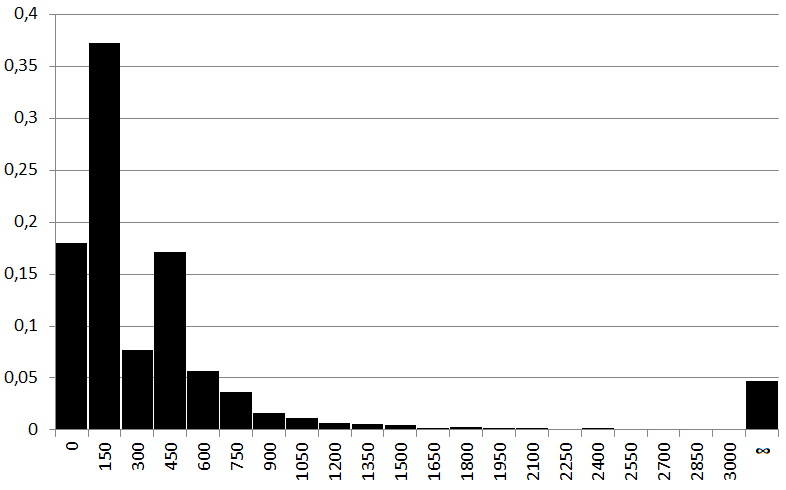
\includegraphics[width=\linewidth]{GraphDeadlock}
    \caption{Гистограмма распределения числа запусков параллельной программ до возникновения взаимоблокировки}
    \label{GraphDeadlock:image}
\end{figure}


Для исправления описанной ошибки нужно сделать порядок захвата замков одинаковым во всех потоках. Иногда советуют во всей программе установить некоторое общее правило захвата замков, например, можно захватывать замки в алфавитном порядке.

Помимо описанной ситуации с неверным порядком захвата мьютексов, существуют и другие причины взаимоблокировок. Например, повторный захват мьютекса (замка). Неверно написанная программа может попытаться повторно захватить уже захваченный ею замок, предварительно его не освободив. При этом повторная попытка захвата полностью останавливает работу потока. Если логика программы требует повторный захват мьютекса (например, для организации рекурсии), следует использовать специальный подвид замков: рекурсивные мьютексы.

\textbf{Состояние гонки (race conditions)} -- ошибка в параллельной программе, при которой результат вычисления зависит от порядка, в котором выполняется код (при каждом запуске параллельной программы он может быть разным). Например, рассмотрим следующую ситуацию. Один поток изменяет значение глобальной переменной. В это время второй поток выводит это значение на печать. Если второй поток напечатает значение раньше, чем его изменит первый, то программа отработает правильно, однако если код выполнится позже, то выведется новое значение, присвоенное в первом потоке.

\begin{minted}{c++}
int a = 0;
#pragma omp parallel num_threads(2) shared(a)
{
    if (omp_get_thread_num() == 0) // first thread 
        a = 2;                     // changes global variable value
    else                           // second thread 
        printf("%d", a);           // print var value: 0 or 2?
}
\end{minted}

С данной проблемой можно столкнуться даже в тех программах, в которых многопоточное программирование не используется явно, но используются какие-то разделяемые ресурсы. Например, если программа копирует текст из поля ввода в буфер обмена и затем тут же вставляется текст в другое поле, то, если она будет запускаться на компьютере одна, то всегда будет работать правильно. Однако если одновременно с ней будет работать программа, также использующая буфер обмена, она может перезаписать значение буфера обмена, даже если команды копирования и вставки будут расположены строго друг за другом. Использование общих ресурсов, даже на очень короткий срок, может привести к ошибке.

Такое явление получило название <<гейзенбаг>> или <<плавающая ошибка>>. Чтобы избежать этой ситуации, надо блокировать запись нового значения переменной в первой потоке, пока второй поток не закончит работу. Например, в технологии OpenMP эту проблему можно решить следующим образом (сохранить старое значение в другой переменной):

\begin{minted}{c++}
int a = 0;
int old_a = a;
#pragma omp parallel num_threads(2) shared(a)
{
    if (omp_get_thread_num() == 0) // first thread 
        a = 2;                     // changes global variable value
    else                           // second thread 
        printf("%d", old_a);       // print old variable value
}
\end{minted}

\textbf{Проблема ABA} -- проблема, при которой поток, два раза читая одинаковое значение, <<думает>>, что данные не изменились. Например, первый поток присвоил переменной значение A. Второй поток присвоил ей значение В, а потом снова А. Когда первый поток снова читает эту переменную, она равна А, и он <<думает>>, что ничего не изменилось. Более практичный пример из программирования: в переменной хранится адрес, указывающий на начало массива. Второй поток освобождает память для нового массива функцией free и создает его функцией malloc, которая выделила память в том же месте, так как эта область памяти уже свободна. Когда первый поток сравнивает значения указателя на массив до и после, он видит, что они равны, и решает, что массив не изменился, хотя на его месте уже хранятся новые данные. Чтобы решить эту проблему, можно хранить признак того, что массив был изменен.

\textbf{Инверсия приоритетов.} Представим ситуацию, в которой существует три потока с приоритетами: высокий, средний и низкий соответственно, причем потоки с высоким и низким приоритетом захватывают общий мьютекс. Пусть поток с низким приоритетом захватил мьютекс и начал свое выполнение, но его прервал поток со средним приоритетом. Теперь, если поток с высоким приоритетом попробует вытеснить поток со средним  приоритетом, он будет ждать освобождения мьютекса, но поток с низким приоритетом не может его освободить, так как его вытеснил поток со средним приоритетом. Эта проблема решается заданием всем потокам одного приоритета на время удержания мьютекса.

\textbf{Голодание (starvation)} возникает, когда поток с низким приоритетом долго находится в состоянии готовности и простаивает. Такое голодание вызвано нехваткой процессорного времени, существует также голодание, вызванное невозможность работы с данными (запрет на чтение и/или запись). В современных ОС эта проблема решается следующим образом: даже если у потока очень низкий приоритет, он все равно вызывается на исполнение через определенное количество времени. В своих программах следует разумно разделять задачи между тредами, чтобы поток, выполняющий более важную и долгую задачу, имел более высокий приоритет.

\textbf{False sharing} -- ситуация, возникающая с системами, поддерживающими когерентность памяти (кэшей), при которой производятся лишние (ненужные в этом месте программы) операции для передачи данных между потоками. \textit{Когерентность памяти (кэшей)} -- свойство памяти, при котором при изменении значения ячейки памяти одним процессом, эти изменения становятся видны в остальных процессах. На организацию такой памяти тратятся большие ресурсы, так как при каждом изменении значения одним потоком, нужно извещать остальные. Рассмотрим следующий пример: 

\inputminted{c++}{listings/falseSharingExample.cpp}

Если запустить функции \code{fprint_a} и \code{fprint_b} в двух разных потоках, то из-за постоянной синхронизации памяти между потоками, программа будет работать медленно, так как a и b находятся в одной строке кэша (обычно 64 байта). Более разумно будет распараллелить каждый цикл между потоками (например, с помощью директивы препроцессора \texttt{\#pragma omp parallel for} в OpenMP).

	\section{Вопросы для самоконтроля усвоенных знаний}

Следующие вопросы позволят оценить степень усвоения знаний с учетом применения лекционного материала и рекомендованной литературы.

\begin{enumerate}
    %%% Лекция 1
    %\item What is the main difference between SMP and MPP systems?
    \item В чем заключается основное различие между SMP- и MPP-системами?
    %\item 4.	During the existence of computer technology, the speed of triggering of elements has increased 10^6 times, and the speed of calculations has increased 10^9 times. How this can happen (means why speed increase in 10^9, not 10^6)?
    \item За время существования вычислительной техники скорость срабатывания элементов увеличилась в $10^6$ раз, а скорость вычислений -- в $10^9$ раз. Как это могло произойти (имеется в виду, почему скорость увеличилась в $10^9$, а не в $10^6$)?
    %\item Assume that you have a program with parallel fraction k = 0.8 and number of processors p = 4. Based on Amdahl’s law calculate parallel speed up S(p) and parallel efficiency EA(p).
    \item Предположим, что имеется программа с параллельной долей $k = 0,8$ и числом процессоров $p = 4$. На основе закона Амдала рассчитайте параллельное ускорение $S(p)$ и параллельную эффективность $E_A(p)$.

    %%% Лекция 2
    %\item You have machine with 4 cores. Thread "A" is running on the 1st core. This thread creates child threads and fibers. Which cores can be used to run such child threads and fibers?
    \item Имеется вычислительная машина с четырьмя ядрами. На первом ядре запущен поток "A". Этот поток создает дочерние потоки и волокна. Какие ядра могут быть использованы для запуска таких дочерних потоков и волокон?
    %\item There is a code that you executed on 4 cores machine.
    % Program was interrupted during execution on thread #3. Which thread will be used to handle additional swap from interrupt_handler?
    \item Имеется код, который выполнялся на вычислительной машине с четырьмя ядрами.
    \begin{minted}{c++}
    __thread int t;
    void swap(int *x, int *y) {
        t = *x;
        *x = *y;
        // hardware interrupt
        *y = t;
    }
    void interrupt_handler() {
        int x = 1, y = 2;
        swap(&x, &y);
    }
    \end{minted}

    Программа была прервана во время выполнения на потоке №3. Какой поток будет использоваться для обработки дополнительного вызова функции swap() от обработчика прерываний?

    %\item How is a thread-safe function different from a reenterable function?
    \item Чем отличается потокобезопасная функция от реентерабельной?

    %\item Specify the main disadvantages of Hyper-Threading.
    \item Укажите основные недостатки использования Hyper-Threading.
    
    %%% Лекция 3
    %\item What is the main difference between instruction and data parallelism?
    \item В чем заключается основное различие между распараллеливанием по данным и распараллеливанием по задачам?

    %\itemFrom the False sharing point of view is it good or bad to have bigger cache memory size? Why?
    \item С точки зрения проблемы False sharing хорошо или плохо иметь больший размер кэш-памяти? Почему?
    
    %\item There is an information about some program:
    %1). Populate an array A (size = 10 elements) with the first 10 elements of Fibonacci sequence. 
    %2). Populate an array B (same size) with elements from array A, but multiply even elements of array A by 2. Array A will not be changed.
    %3). Summarize elements of array A -> variable C.
    %4). Summarize elements of array B -> variable D.
    %5). Compare variables C and D. 

    %Which parallelization can be used (data, instructions, information flows) and why?
    \item Имеется информация о некоторой программе:
    \begin{enumerate}
        \item Заполнить массив A (размер = 10 элементов) первыми 10 элементами последовательности Фибоначчи. 
        \item Заполнить массив B (того же размера) элементами из массива A, но четные элементы массива A умножить на 2. Массив A не изменяется.
        \item Просуммировать элементы массива A и записать в переменную C.
        \item Просуммировать элементы массива B и записать в переменную D.
        \item Сравнить переменные C и D. 
    \end{enumerate}
    
    Какое распараллеливание можно использовать (по данным, по задачам, по информационным потокам) и почему?


    %%% Лекция 4
    %\item Modify the following sequential program by adding openmp constructions in order to be parallelized on proper amount of threads:

    \item Используя информацию о программе из предыдущего вопроса, модифицируйте следующую последовательную программу, добавив конструкции OpenMP, чтобы распараллелить ее на соответствующее число потоков:
    \begin{minted}{c++}
    populate_array(A);
    populate_array(B);
    sum_elements_array(A, C);
    sum_elements_array(B, D);
    compare(C, D)
    \end{minted}
   
    
    %\item What is the main difference between forward and backward compatibility?
    \item В чем заключается основное различие между прямой и обратной совместимостью?

    
    %%% Лекция 5
    %\item The following program is used to calculate number s as the sum of integers from 0 to 49. The program is compiled using OpenMP technology and runs on a dual-core processor. Why is the program giving the wrong result?
    \item Следующая программа используется для вычисления числа $s$ как суммы целых чисел от 0 до 50. Программа скомпилирована с использованием технологии OpenMP и выполняется на двухъядерном процессоре.

    \begin{minted}{c++}
    #include <stdio.h>
    #include <omp.h>
    void main(int argc, char* argv[]) {
        int s = 0, i = 0;
        #pragma omp parallel for
        for (int i = 0; i < 49; i++) s += i;
        printf("s = %d\n", s);
    }
    \end{minted}
    
    
    Почему программа выдает неверный результат?

    %\item How can you change the program from the previous question to give the correct result and use OpenMP's paralleling capabilities to find the sum? Provide all possible solutions.
    \item Как можно изменить программу из предыдущего вопроса, чтобы получить правильный результат и использовать возможности распараллеливания OpenMP для нахождения суммы? Приведите все возможные решения.
    
    %%% Лекция 6
    % \item Name the main differences between the master directive and the single directive
    %\item Перечислите основые отличие между директивой <<omp master>> и <<omp single>> в OpenMP.

    % \item Why nested style is faster than cascade one?
    \item Почему при использовании большого числа циклов в OpenMP время выполнения программы быстрее при использовании вложенного стиля?

    % \item What value n will be printed on the console?
    % \item What happens if firstprivate will be used instead of lastprivate?
    % \item What happens if private will be used instead of lastprivate?
    \item На основе следующего кода ответьте на несколько вопросов:
    \begin{minted}{c++}
    int n = 0;
    printf("Значение n в начале: %d\n", n);
    #pragma omp parallel for lastprivate(n)
    for (int i = 0; i < 6; ++i) {
        n = i * 10;
    }
    printf("Значение n в конце: %d\n", n);
    \end{minted}

    \begin{enumerate}[label*=\arabic*.]
        \item Какое значение $n$ будет выведено в конце?
        \item Как изменится значение $n$ в конце, если <<lastprivate>> заменить на <<firstprivate>>?
        \item Как изменится значение $n$ в конце, если <<lastprivate>> заменить на <<private>>?
    \end{enumerate}
    
    %%% Лекция 7
    % \item How many threads can be involved in deadlock? Explain your answer
     \item Какое число потоков необходимо для возможного появления взаимной блокировки? Объясните ответ.

     % \item What does transactional memory mean? Give examples of usage.
     \item Что такое программная транзакционная память? Приведите пример использования.

     % \item With the help of what function in POSIX THREAD the thread pool is merged (when one thread is waiting for another thread to finish).
     \item С помощью какой функции в POSIX Threads происходит слияние пула потоков (когда один поток ожидает завершения другого потока).
     
    
    %%% Лекция 8
    % \item You have an array of 317 element. Local work size = 12. Specify work_group_id and local_id for element 134
    \item Имеется массив из 317 элементов, который обрабатывается с помощью OpenCL, значение local\_work\_size = 12. Укажите work\_group\_id and local\_id для элемента с индексом 134.
    
    % \item Specify OpenCL memory types. How do they relate to each other?
    \item Перечислите типы памяти, существующие в OpenCL. Есть ли особенности взаимодействия разных типов памяти?
\end{enumerate} 
	\section{Лабораторная работа №1. <<Автоматическое распараллеливание программ>>}
\subsection{Порядок выполнения работы}
\begin{enumerate}
    \itemНа компьютере с многоядерным процессором установить Unix-подобную операционную систему и компилятор GCC версии не ниже 9.x. При невозможности установить Unix-подобную операционную систему или отсутствии компьютера с многоядерным процессором можно выполнять лабораторную работу на виртуальной машине. Минимальное число ядер при использовании виртуальной машины -- два. Важным условием является отключение гипертрединга, для того, чтобы выполнить честные замеры времени. 
    
    \item На языке Cи написать консольную программу lab1.c, решающую задачу, указанную в п.~5.5 (см. ниже). В программе нельзя использовать библиотечные функции сортировки, выполнения матричных операций и расчёта статистических величин. В программе нельзя использовать библиотечные функции, отсутствующие в стандартных заголовочных файлах stdio.h, stdlib.h, sys/time.h, math.h. Задача должна решаться 100 раз с разными начальными значениями генератора случайных чисел (ГСЧ). Структура программы примерно следующая:

    \inputminted[fontsize=\footnotesize]{c++}{listings/lab1Example.cpp}

    \itemСкомпилировать написанную программу без использования автоматического распараллеливания с помощью следующей команды: 
    
    \mint[breaklines]{text}{/home/user/gcc -O3 -Wall -Werror -lm -o lab1-seq lab1.c}
    
    \itemСкомпилировать написанную программу, используя встроенное в gcc средство автоматического распараллеливания Graphite, с помощью следующей команды:
    
    \mint[breaklines]{text}{/home/user/gcc -O3 -Wall -Werror -lm -floop-parallelize-all -ftree-parallelize-loops=K lab1.c -o lab1-par-K} 
    
    \noindent(переменной K поочерёдно присвоить хотя бы четыре значения: один, меньше числа физических ядер, равное числу физических ядер и больше числа физических ядер).
    
    \itemВ результате получится одна нераспараллеленная программа и четыре или более распараллеленных.
    \itemЗакрыть все работающие в операционной системе прикладные программы (включая Winamp, uTorrent, браузеры, Telegram и Skype), чтобы они не влияли на результаты последующих экспериментов. При использовании ноутбука \textbf{необходимо иметь постоянное подключение к сети питания} на время проведения эксперимента.
    
    \itemЗапускать файл lab1-seq из командной строки, увеличивая значения N до значения N1, при котором время выполнения превысит 0.01 с. Подобным образом найти значение N=N2, при котором время выполнения превысит 5 с.
    
    \itemИспользуя найденные значения N1 и N2, выполнить следующие эксперименты (для автоматизации проведения экспериментов рекомендуется написать скрипт):
    
    \begin{itemize}
        \itemзапускать lab1-seq для значений \\ $N = {N1, N1 + \Delta, N1 + 2 \Delta, N1 + 3 \Delta, \dots, N2}$ и записывать получающиеся значения времени \code{delta_ms(N)} в функцию \code{seq(N)};
        \itemзапускать lab1-par-K для значений \\ $N = {N1, N1 + \Delta, N1 + 2 \Delta, N1 + 3 \Delta, \dots, N2}$ и записывать получающиеся значения времени \code{delta_ms(N)} в функцию \code{par-K(N)};
        \itemзначение $\Delta$ выбрать так: $\Delta = (N2 - N1) / 10$.
    \end{itemize}
    
    \itemПровести верификацию значения X. Добавить в конец цикла вывод значения X и изменить число экспериментов на 5. Сравнить значения X для распараллеленной программы и нераспараллеленной.
    
    \itemНаписать отчёт о проделанной работе.
    
    \itemПодготовиться к устным вопросам на защите.
    
    \itemНайти вычислительную сложность алгоритма до и после распараллеливания, сравнить полученные результаты.
    
    \item\textbf{Необязательное задание №1 (для получения оценки <<4>> и <<5>>).} Провести аналогичные описанным эксперименты, используя вместо gcc компилятор Solaris Studio (или любой другой на своё усмотрение). При компиляции следует использовать следующие опции для автоматического распараллеливания: 
    \mint[breaklines]{text}{solarisstudio -cc -O3 -xautopar -xloopinfo lab1.c}
    
    \item\textbf{Необязательное задание №2 (для получения оценки <<5>>).} Это задание выполняется только после выполнения предыдущего пункта. Провести аналогичные описанным эксперименты, используя вместо gcc компилятор Intel ICC (или любой другой на своё усмотрение). В ICC следует при компиляции использовать следующие опции для автоматического распараллеливания: 
    \mint[breaklines]{text}{icc -parallel -par-threshold=0 -par-num-threads=K -o lab1-icc-par-K lab1.c}
\end{enumerate}

\subsection{Состав отчета}
\begin{enumerate}
    \itemТитульный лист с названием вуза, ФИО студента и названием работы.
    \itemСодержание отчета (с указанием номера страниц и т.п.).
    \itemОписание решаемой задачи (взять из п.~5.5).
    \itemКраткая характеристика использованного для проведения экспериментов процессора, операционной системы и компилятора GCC (официальное название, номер версии/модели, разрядность, число ядер, ёмкость ОЗУ, размер кэша и т.п.).
    \itemПолный текст программы lab1.c в виде отдельного файла.
    \itemТаблицы значений и графики функций seq(N), par-K(N) с указанием времени выполнения и величины параллельного ускорения. Предпочтительно использовать столбчатые гистограммы, показывающие зависимости времени или ускорения от размера массива.
    \itemПодробные выводы с анализом приведённых графиков и полученных результатов.
    \itemОтчёт предоставляется в бумажном или электронном виде вместе с полным текстом программы. По требованию преподавателя нужно быть готовыми скомпилировать и запустить этот файл на компьютере в учебной аудитории (или своём ноутбуке).
\end{enumerate}

\subsection{Вопросы для самопроверки}
\begin{enumerate}
    \item На что влияет параметр \code{seed}?
    \item Для чего может понадобиться ключ \code{-lm}?
    \item Почему значения X могут отличаться для последовательной и для параллельной программ?
    \item Параллельное ускорение составило 0.1. Когда возможна такая ситуация, и о чём это свидетельствует?
    \item В каком случае значение параллельной эффективности будет больше значения параллельного ускорения для некоторой программы на некоторой вычислительной машине?
\end{enumerate}

\subsection{Подготовка к защите}

\begin{enumerate}
    \itemУметь объяснить каждую строку программы, представленной в отчёте.
    \itemЗнать о назначении и основных особенностях GCC, а также о назначении всех использованных в работе ключей компиляции GCC.
    \itemЗнать материал лекции №1.
    \itemВзять с собой все нужные файлы для демонстрации работы программы.
\end{enumerate}
\subsection{Варианты заданий}

Вариант задания выбирается в соответствии с приведёнными ниже описанием этапов, учитывая, что число А = Ф*И*О, где Ф, И, О означают число букв в фамилии, имени и отчестве студента. Номер варианта в соответствующих таблицах выбирается по формуле X = 1 + ((A mod 47) mod B), где В -- число элементов в соответствующей таблице, а операция mod означает остаток от деления. Например, при А = 476 и В = 5, получим \textbf{Х = 1 + ((470 + 6) mod 47) mod 5) = 1 + (6 mod 5) = 2}. Порядок вычислений должен быть следующим:

\begin{enumerate}
    \item\textbf{Этап Generate.} Сформировать массив М1 размерностью N, заполнив его с помощью функции \code{rand_r} (нельзя использовать \code{rand}) случайными вещественными числами, имеющими равномерный закон распределения в диапазоне от 1 до A (включительно). Аналогично сформировать массив М2 размерностью N/2 со случайными вещественными числами в диапазоне от А до 10*А.
    \item\textbf{Этап Map.} В массиве М1 к каждому элементу применить операцию из таблицы:

    % \begin{enumerate}
    %     \item[1.] Гиперболический синус с последующим возведением в квадрат
    %     \item[2.] Гиперболический косинус с последующим увеличением на 1
    %     \item[3.] Гиперболический тангенс с последующим уменьшением на 1
    %     \item[4.] Гиперболический котангенс корня числа
    %     \item[5.] Деление на Пи с последующим возведением в третью степень
    %     \item[6.] Кубический корень после деления на число e
    %     \item[7.] Экспонента квадратного корня (т.е. M1[i] = exp(sqrt(M1[i])))
    % \end{enumerate}
    
    \begin{center}
        \begin{tabular}{|c|c|}
            \hline
            \thead{Номер \\ варианта} & \thead{Операция} \\ \hline
            1 & \makecell{Гиперболический синус с последующим\\ возведением в квадрат} \\ \hline
            2 & \makecell{Гиперболический косинус с последующим\\ увеличением на 1} \\ \hline
            3 & \makecell{Гиперболический тангенс с последующим\\ уменьшением на 1} \\ \hline
            4 & \makecell{Гиперболический котангенс\\ корня числа} \\ \hline
            5 & \makecell{Деление на Пи с последующим возведением\\ в третью степень} \\ \hline
            6 & \makecell{Кубический корень после деления\\ на число e} \\ \hline
            7 & \makecell{Экспонента квадратного корня\\ (т.е. M1[i] = exp(sqrt(M1[i])))} \\ \hline
        \end{tabular}
    \end{center}
        
    Затем в массиве М2 каждый элемент поочерёдно сложить с предыдущим (для этого вам понадобится копия массива М2, из которого нужно будет брать операнды), а к результату сложения применить операцию из таблицы (считать, что для начального элемента массива предыдущий элемент равен нулю):
    
    \begin{center}
        \begin{tabular}{|c|c|}
            \hline
            \thead{Номер \\ варианта} & \thead{Операция} \\ \hline
            1 & Модуль синуса (т.е. M2[i] = |sin(M2[i] + M2[i-1])|) \\ \hline
            2 & Модуль косинуса \\ \hline
            3 & Модуль тангенса \\ \hline
            4 & Модуль котангенса \\ \hline
            5 & Натуральный логарифм модуля тангенса \\ \hline
            6 & Десятичный логарифм, возведенный в степень e \\ \hline
            7 & Кубический корень после умножения на число Пи \\ \hline
            8 & Квадратный корень после умножения на e \\ \hline
        \end{tabular}
    \end{center}
    
    \item\textbf{Этап Merge.} В массивах М1 и М2 ко всем элементами с одинаковыми индексами попарно применить операцию из таблицы (результат записать в М2): 

    \begin{center}
        \begin{tabular}{|c|c|}
            \hline
            \thead{Номер \\ варианта} & \thead{Операция} \\ \hline
            1 & Возведение в степень (т.е. M2[i] = M1[i]\verb+^+M2[i]) \\ \hline
            2 & Деление (т.е. M2[i] = M1[i]/M2[i]) \\ \hline
            3 & Умножение \\ \hline
            4 & Выбор большего (т.е. M2[i] = max(M1[i],M2[i]))) \\ \hline
            5 & Выбор меньшего \\ \hline
            6 & Модуль разности \\ \hline
        \end{tabular}
    \end{center}
    
    \item\textbf{Этап Sort.} Полученный массив необходимо отсортировать методом, указанным в таблице (для этого нельзя использовать библиотечные функции; можно взять реализацию в виде свободно доступного исходного кода):
        \begin{center}
            \begin{tabular}{|c|c|}
                \hline
                \thead{Номер \\ варианта} & \thead{Операция} \\ \hline
                1 & Сортировка выбором (Selection sort) \\ \hline
                2 & Сортировка расчёской (Comb sort) \\ \hline
                3 & \makecell{Пирамидальная сортировка (HeapSort, \\ сортировка кучи)} \\ \hline
                4 & Гномья сортировка (Gnome sort) \\ \hline
                5 & Сортировка вставками (Insertion sort) \\ \hline
                6 & Сортировка выбором (Selection sort) \\ \hline
            \end{tabular}
        \end{center}
    \item\textbf{Этап Reduce.} Рассчитать сумму синусов тех элементов массива М2, которые при делении на минимальный ненулевой элемент массива М2 дают чётное число (при определении чётности учитывать только целую часть числа). Результатом работы программы по окончании пятого этапа должно стать одно число X, которое следует использовать для верификации программы после внесения в неё изменений (например, до и после распараллеливания итоговое число X не должно измениться в пределах погрешности). Данное число необходимо выводить на каждой итерации на этапе верификации. Значение числа X следует привести в отчёте для различных значений N. 
    \par
\end{enumerate}


	\section{Лабораторная работа №2. <<Исследование эффективности параллельных библиотек для С-программ>>}
\subsection{Порядок выполнения работы}
\begin{enumerate}
    \itemВ исходном коде программы, полученной в результате выполнения лабораторной работы №1, нужно на этапах Map и Merge все циклы с вызовами математических функций заменить их векторными аналогами из библиотеки <<AMD Framewave>>\footnote{\url{http://framewave.sourceforge.net}}. При выборе конкретной Framewave-функции необходимо убедиться, что она помечена как MT\footnote{Multi-Threaded, т.е. распараллеленная}. Полный перечень доступных функций находится по ссылке: \url{http://framewave.sourceforge.net/Manual/fw_section_060.html#fw_section_060}. \quad Например, Framewave-функция min в списке поддерживаемых технологий имеет только SSE2, но не MT\@. 
	
    \textit{Примечание:} выбор библиотеки Framewave не является обязательным, можно использовать любую другую параллельную библиотеку, если в ней нужные функции распараллелены, так, например, можно использовать ATLAS (для этой библиотеки необходимо выключить троттлинг и энергосбережение, а также разобраться с механизмом изменения числа потоков) или Intel Integrated Performance Primitives.
	
    \itemДобавить в начало программы вызов Framewave-функции \code{SetNumThreads(M)} для установки количества M создаваемых параллельной библиотекой потоков, задействуемых при выполнении распараллеленных Framewave-функций. Нужное число M следует устанавливать из параметра командной строки (argv) для удобства автоматизации экспериментов.
	
    \textit{Примечание:} В случае использования Intel IPP не нужно использовать функцию \code{SetNumThreads(M)}. Необходимо компилировать программу под разное количество потоков.
	
    Скомпилировать программу, не применяя опции автоматического распараллеливания, использованные в лабораторной работе №1. Провести эксперименты с полученной программой для тех же значений $N_1$ и $N_2$, которые использовались в лабораторной работе №1, при M = 1, 2, \ldots , K, где K –- число процессоров (ядер) на экспериментальном стенде.
		
    \itemСравнить полученные результаты с результатами лабораторной работы №1: на графиках показать, как изменилось время выполнения программы, параллельное ускорение и параллельная эффективность.
		
    \itemНаписать отчёт о проделанной работе.
		
    \itemПодготовиться к устным вопросам на защите.
		
    \item\textbf{Необязательное задание №1 (для получения оценки <<4>> и <<5>>).} Исследовать параллельное ускорение для различных значений M > K, т.е. оценить накладные расходы при создании чрезмерного большого числа потоков. Для иллюстрации того, что программа действительно распараллелилась, привести график загрузки процессора (ядер) во время выполнения программы при $N = N_2$ для всех использованных M. Для получения графика можно как написать скрипт, так и просто сделать скриншот диспетчера задач, указав на скриншоте моменты начала и окончания эксперимента (в отчёте нужно привести текст скрипта или название использованного диспетчера).
		
    \item\textbf{Необязательное задание №2 (для получения оценки <<5>>).} Это задание выполняется только после выполнения предыдущего пункта. Используя закон Амдала, рассчитать коэффициент распараллеливания для всех экспериментов и привести его на графиках. Прокомментировать полученные результаты.
\end{enumerate}

\subsection{Состав отчета}
\begin{enumerate}
    \itemТитульный лист с названием вуза, ФИО студентов и названием работы.
    \itemСодержание отчета (с указанием номера страниц и т.п.).
    \itemКраткая характеристика использованного для проведения экспериментов процессора, операционной системы и компилятора (официальное название, номер версии/модели, разрядность, число ядер, ёмкость ОЗУ, размер кэша и т.п.).
    \itemОписание особенностей конфигурации использованной параллельной библиотеки, включая описание последовательности шагов, предпринятых для установки библиотеки, и использованных опций компиляции.
    \itemПолный текст полученной параллельной программы, а также текст всех скриптов, использованных для компилирования программы и проведения экспериментов.
    \itemГрафики функций времени выполнения использованных программ, а также графики параллельного ускорения и параллельной эффективности для разных N и M (допускается совмещать несколько графиков в одной системе координат). Предпочтительно использовать столбчатые гистограммы.
    \itemПодробные выводы с анализом приведённых графиков и полученных результатов.
    \itemОтчёт предоставляется в бумажном или электронном виде вместе с полным текстом программы. По требованию преподавателя нужно быть готовыми скомпилировать и запустить этот файл на компьютере в учебной аудитории (или своём ноутбуке).
\end{enumerate}

\subsection{Вопросы для самопроверки}
\begin{enumerate}
    \item Как посчитать долю кода, который можно распараллелить, если известны ускорение и число потоков?
    \item Математические функции в библиотеках имеют разрядность 32 и 64 бита. Что будет, если использовать в программе комбинацию таких функций? Например, power32 и abs64.
\end{enumerate}

\subsection{Подготовка к защите}
\begin{enumerate}
    \itemУметь объяснить каждую строку программы, представленной в отчёте.
    \itemЗнать о назначении всех использованных в работе ключей компиляции.
    \itemЗнать материал лекций №2-3.
    \itemВзять с собой все нужные файлы для демонстрации работы программы.
\end{enumerate}


	\section{Лабораторная работа №3. <<Распараллеливание циклов с помощью технологии OpenMP>>}
\label{sec:lab3-openmp}
\subsection{Порядок выполнения работы}
\begin{enumerate}
    \itemДобавить во все for-циклы (кроме цикла в функции main, указывающего количество экспериментов) в программе из ЛР №1 следующую директиву OpenMP:
    \mint{c++}|#pragma omp parallel for default(none) private(...) shared(...)|
    Наличие параметра \code{default(none)} является обязательным.
    
    \itemПроверить все for-циклы на внутренние зависимости по данным между итерациями. Если зависимости обнаружились, использовать для защиты критических секций директиву <<\#pragma omp critical>> или <<\#pragma omp atomic>> (если операция атомарна), или параметр reduction (предпочтительнее), или вообще отказаться от распараллеливания цикла (свой выбор необходимо обосновать).
    
    \itemУбедиться, что получившаяся программа обладает свойством прямой совместимости с компиляторами, не поддерживающими OpenMP (для проверки этого можно скомпилировать программу без опции <<–fopenmp>>, в результате не должно быть сообщений об ошибках, а программа должна корректно работать).
    
    \itemИспользовать функцию SetNumThreads для изменения числа потоков. В отчете указать максимальное количество потоков.
    
    \itemПровести эксперименты, замеряя параллельное ускорение. Привести сравнение графиков параллельного ускорения с ЛР~№1 и ЛР~№2.
    
    \itemПровести эксперименты, добавив параметр <<schedule>> и варьируя в экспериментах тип расписания. Исследование нужно провести для всех возможных расписаний: static, dynamic, guided. Следующей <<степенью свободы>>, которую необходимо использовать, является chunck\_size, которому необходимо задать четыре различных варианта: единице, меньше чем число потоков, равному числу потоков и больше чем число потоков. Привести сравнение параллельного ускорения при различных расписаниях с результатами п.~5.
    
    \itemОпределить, какой тип расписания на вычислительной машине при использовании <<schedule default>>.
    
    \itemВыбрать из рассмотренных в п.~5 и п.~6 наилучший вариант при различных N. Сформулировать условия, при которых наилучшие результаты получились бы при использовании других типов расписания.
    
    \itemНайти вычислительную сложность алгоритма до и после распараллеливания, сравнить полученные результаты.
    
    \itemДля иллюстрации того, что программа действительно распараллелилась, привести график загрузки процессора (ядер) от времени при выполнении программы при $N = N_1$ для лучшего варианта распараллеливания. Для получения графика можно как написать скрипт, так и просто сделать скриншот диспетчера задач, указав на скриншоте моменты начала и окончания эксперимента (в отчёте нужно привести текст скрипта или название использованного диспетчера). Недостаточно привести однократное моментальное измерение загрузки утилитой htop, т.к. требуется привести график изменения загрузки за всё время выполнения программы.
    
    \itemНаписать отчёт о проделанной работе.
    
    \itemПодготовиться к устным вопросам на защите.
    
    \item\textbf{Необязательное задание №1 (для получения оценки <<4>> и <<5>>).} Построить график параллельного ускорения для точек $N < N_1$ и найти значения $N$, при которых накладные расходы на распараллеливание превышают выигрыш от распараллеливания (независимо для различных типов расписания).
    
    \item \textbf{Необязательное задание №2 (для получения оценки <<5>>).} Для лучшего результата по итогам всех экспериментов сделать еще минимум три эксперимента, заменив флаг <<-O3>> на другие флаги оптимизации. Построить график времени выполнения от $N$.
\end{enumerate}
\subsection{Состав отчета}
\begin{enumerate}
    \itemТитульный лист с названием вуза, ФИО студентов и названием работы.
    \itemСодержание отчета (с указанием номера страниц и т.п.).
    \itemКраткое описание решаемой задачи.
    \itemХарактеристика использованного для проведения экспериментов процессора, операционной системы и компилятора GCC (точное название, номер версии/модели, разрядность, размер кэша, число ядер и т.п.).
    \itemМаксимальное число потоков, которое можно создать на данной вычислительной машине.
    \itemПолный текст программы с использованием параметра schedule.
    \itemПодробные выводы с анализом каждого из приведённых графиков.
    \itemОтчёт предоставляется в бумажном или электронном виде вместе с полным текстом программы. По требованию преподавателя нужно быть готовыми скомпилировать и запустить этот файл на компьютере в учебной аудитории (или своём ноутбуке).
\end{enumerate}

\subsection{Вопросы для самопроверки}
\begin{enumerate}
    \item Как узнать значение default chuck size?
    \item Как доказать, что необязательное задание №2 (п.~14) работает независимо от расписаний?
\end{enumerate}

\subsection{Подготовка к защите}
\begin{enumerate}
    \itemУметь объяснить каждую строку программы, представленной в отчёте.
    \itemУметь объяснить выводы, полученные в результате работы.
    \itemЗнать назначение каждой директивы OpenMP, использованной в программе.
    \itemПовторить материал лекций №4-6, прочитать главу про OpenMP в методическом пособии
    \itemПрочитать материал о директиве <<\#pragma omp for>> в книге Антонова <<Параллельное программирование с использованием технологии OpenMP: Учебное пособие>>~\cite{AntonovOpenMP2004}, знать ответы на вопросы в конце соответствующей главы.
\end{enumerate}


	\section{Лабораторная работа №4. <<Метод доверительных интервалов при измерении времени выполнения параллельной OpenMP-программы>>}
\label{sec:lab4-openmp}
\subsection{Порядок выполнения работы}
\begin{enumerate}
    \itemВ программе, полученной в результате выполнения ЛР №3, так изменить этап Generate, чтобы генерируемый набор случайных чисел не зависел от числа потоков, выполняющих программу. Например, на каждой итерации i перед вызовом \code{rand_r} можно вызывать функцию \code{srand(f(i))}, где f -– произвольно выбранная функция. Можно придумать и использовать любой другой способ.
    
    \itemЗаменить вызовы функции \code{gettimeofday} на \code{omp_get_wtime}.
    
    \itemРаспараллелить вычисления на этапе Sort, для чего выполнить сортировку в два этапа: 
    \begin{itemize}
        \itemОтсортировать первую и вторую половину массива в двух независимых нитях (можно использовать OpenMP-ди\-рек\-ти\-ву <<parallel sections>>).
        \itemОбъединить отсортированные половины в единый массив.
    \end{itemize}
    
    \itemНаписать функцию, которая один раз в секунду выводит в консоль сообщение о текущем проценте завершения работы программы. Указанную функцию необходимо запустить в отдельном потоке, параллельно работающем с основным вычислительным циклом. Нельзя использовать PThreads, сделать только средствами OpenMP.
    
    \itemОбеспечить прямую совместимость (forward compatibility) написанной параллельной программы. Для этого все вызываемые функции вида <<omp\_*>> можно условно переопределить в препроцессорных директивах, например, так:
    
    \begin{minted}{c++}
    #ifdef _OPENMP
        #include <omp.h>
    #else
        int omp_get_num_procs() { return 1; }
    #endif
    \end{minted}
    
    \itemПровести эксперименты, варьируя $N$ от $\min({N_x}/{2}, N_1)$ до $N_2$, где значения $N_1$ и $N_2$ взять из ЛР №1, а $N_x$ –- это такое значение $N$, при котором накладные расходы на распараллеливание превышают выигрыш от распараллеливания. Написать отчёт о проделанной работе. Подготовиться к устным вопросам на защите.
    
    \item\textbf{Необязательное задание №1 (для получения оценки <<4>> и <<5>>).} Уменьшить число итераций основного цикла с 100 до 10 и провести эксперименты, замеряя время выполнения следующими методами: 
        \begin{itemize}
            \itemИспользование минимального из десяти полученных замеров. 
            \itemРасчёт по десяти измерениям доверительного интервала с уровнем доверия 95\%.
        \end{itemize}
        Привести графики параллельного ускорения для обоих методов в одной системе координат, при этом нижнюю и верхнюю границу доверительного интервала следует привести двумя независимыми графиками.
    
    \item\textbf{Необязательное задание №2 (для получения оценки <<5>>).} В п.~3 задания на этапе Sort выполнить параллельную сортировку не двух частей массива, а $k$ частей в $k$ нитях (тредах), где $k$ –- это число процессоров (ядер) в системе, которое становится известным только на этапе выполнения программы с помощью команды:
    \mint{c++}{int k = omp_get_num_procs()}
\end{enumerate}

\subsection{Состав отчета}

\begin{enumerate}
    \itemТитульный лист с названием вуза, ФИО студентов и названием работы.
    \itemСодержание отчета (с указанием номера страниц и т.п.).
    \itemКраткое описание решаемой задачи.
    \itemХарактеристика использованного для проведения экспериментов процессора, операционной системы и компилятора GCC (точное название, номер версии/модели, разрядность, число ядер и т.п.).
    \itemПолный текст программы и использованных в процессе работы скриптов и инструментов с указанием параметров запуска.
    \itemПодробные выводы с анализом каждого из приведённых графиков.
    \itemОтчёт предоставляется в бумажном или электронном виде вместе с полным текстом программы. По требованию преподавателя нужно быть готовыми скомпилировать и запустить этот файл на компьютере в учебной аудитории (или своём ноутбуке).
\end{enumerate}

\subsection{Вопросы для самопроверки}
\begin{enumerate}
    \item В чём особенность различных функций измерения времени?
    \item Какие ещё способы вызова функции о проценте завершения можно предложить? В чём преимущества и недостатки каждого из способов?
\end{enumerate}

\subsection{Подготовка к защите}

\begin{enumerate}
    \itemУметь объяснить каждую строку программы, представленной в отчёте.
    \itemУметь объяснить выводы, полученные в результате работы.
    \itemЗнать назначение каждой директивы OpenMP, использованной в программе.
    \itemПовторить материал лекций №4-6, прочитать главу про OpenMP в методическом пособии.
    \itemЗнать ответы на вопросы из разделов <<Задание>> книги Антонова <<Параллельное программирование с использованием технологии OpenMP: Учебное пособие>> (см. страницы 12, 28, 35, 54)~\cite{AntonovOpenMP2004}.
\end{enumerate}


	\section{Лабораторная работа №5. <<Параллельное программирование с использованием стандарта POSIX Threads>>}
\subsection{Порядок выполнения работы}
\begin{enumerate}
    \itemВзять в качестве исходной OpenMP-программу из ЛР №4, в которой распараллелены все этапы вычисления. Убедиться, что в этой программе корректно реализован одновременный доступ к общей переменной, используемой для вывода в консоль процента завершения программы.
    \itemИзменить исходную программу так, чтобы вместо OpenMP-ди\-рек\-тив применялся стандарт <<POSIX Threads>>:
        \begin{itemize}
            \item\textbf{для получения оценки <<3>>} достаточно изменить только один этап (Generate, Map, Merge, Sort), который является узким местом (bottleneck), а также функцию вывода в консоль процента завершения программы;
            \item\textbf{для получения оценки <<4>> и <<5>>} необходимо изменить всю программу, но допускается в качестве расписания циклов использовать <<schedule static>>;
            \item\textbf{для получения оценки <<5>>} необходимо хотя бы один цикл распараллелить, реализовав вручную расписание <<schedule dynamic>> или <<schedule guided>>.
        \end{itemize}
    \itemПровести эксперименты и по результатам выполнить сравнение работы двух параллельных программ (<<OpenMP>> и <<POSIX Threads>>), которое должно описывать следующие аспекты работы обеих программ (для различных $N$):
        \begin{itemize}
            \itemполное время решения задачи;
            \itemпараллельное ускорение;
            \itemдоля времени, проводимого на каждом этапе вычисления (<<нормированная
диаграмма с областями и накоплением>>);
            \itemколичество строк кода, добавленных при распараллеливании, а также грубая оценка
времени, потраченного на распараллеливание (накладные расходы программиста);
            \itemостальные аспекты, которые вы выяснили самостоятельно \textbf{(обязательный пункт)}.
        \end{itemize}
\end{enumerate}

\subsection{Состав отчета}

\begin{enumerate}
    \itemТитульный лист с названием вуза, ФИО студентов и названием работы. 
    \itemСодержание отчета (с указанием номера страниц и т.п.).
    \itemКраткое описание решаемой задачи.
    \itemХарактеристика использованного для проведения экспериментов процессора, операционной системы и компилятора GCC (точное название, номер версии/модели, разрядность, число ядер и т.п.).
    \itemПолный текст программ (<<OpenMP>> и <<POSIX Threads>>) и использованных в процессе работы скриптов, и инструментов с указанием параметров запуска.
    \itemПодробные выводы с анализом каждого из приведённых графиков.
    \itemОтчёт предоставляется в бумажном или электронном виде вместе с полным текстом программы. По требованию преподавателя нужно быть готовыми скомпилировать и запустить этот файл на компьютере в учебной аудитории (или своём ноутбуке).
\end{enumerate}
\subsection{Вопросы для самопроверки}
\begin{enumerate}
    \item Для чего используется функция \code{pthread_exit()} и можно ли обойтись без неё?
    \item Какие атрибуты можно передать в функцию \code{pthread_create()}?
\end{enumerate}

\subsection{Подготовка к защите}

\begin{enumerate}
    \itemУметь объяснить каждую строку программы, представленной в отчёте. 
    \itemУметь объяснить выводы, полученные в результате работы.
    \itemПодготовиться к ответам на вопросы по материалам лекции №7.
\end{enumerate}


	\section{Лабораторная работа №6. <<Изучение технологии OpenCL>>}
\subsection{Порядок выполнения работы}

\begin{enumerate}
    \itemВам необходимо реализовать один (для оценки <<3>>) или два (для оценки <<4>>) этапа вашей программы из предыдущих лабораторных работ. При этом вычисления можно проводить как на CPU, так и на GPU (на своё усмотрение, но GPU предпочтительнее).
    \item\textbf{Необязательное задание №1 (для получения оценки <<5>>).}
        \begin{itemize}
            \itemВыполнение заданий для оценки <<3>> и <<4>>.
            \itemРасчёт доверительного интервала. 
            \itemПосчитать время двумя способами: с помощью profiling и с помощью обычного замера (как в предыдущих заданиях).
            \itemОценить накладные расходы, такие как доля времени, проводимого на каждом этапе вычисления (<<нормированная диаграмма с областями и накоплением>>), число строк кода, добавленных при распараллеливании, а также грубая оценка времени, потраченного на распараллеливание (накладные расходы программиста), и т.п.
        \end{itemize}
    \item\textbf{Необязательное задание №2 (для получения бонусов и лучшей итоговой оценки по итогам прохождения дисциплины).} Провести вычисления совместно на GPU и CPU (т.е. итерации в некоторой обоснованной пропорции делятся между GPU и CPU, и параллельно на них выполняются).
    \itemПри желании данную лабораторную работу можно написать на CUDA.
\end{enumerate}


\subsection{Состав отчета}
\begin{enumerate}
    \itemТитульный лист с названием вуза, ФИО студентов и названием работы. Содержание отчета (с указанием номера страниц и т.п.).
    \itemКраткое описание решаемой задачи.
    \itemХарактеристика использованного для проведения экспериментов процессора, операционной системы и компилятора GCC (точное название, номер версии/модели, разрядность, число ядер и т.п.).
    \itemПолный текст распараллеленной программы (для п.~2 и п.~3).
    \itemПодробные выводы.
    \itemОтчёт предоставляется в бумажном или электронном виде вместе с полным текстом программы. По требованию преподавателя нужно быть готовыми скомпилировать и запустить этот файл на компьютере в учебной аудитории (или своём ноутбуке).
\end{enumerate}


\subsection{Вопросы для самопроверки}
\begin{enumerate}
    \item Есть вычислительная машина с графическим процессором. Какой процессор будет выбран в случае использования CL\_DEVICE\_TYPE\_DEFAULT?
    \item Каким способом можно сократить накладные расходы?
\end{enumerate}

\subsection{Подготовка к защите}
\begin{enumerate}
    \itemУметь объяснить каждую строку программы, представленной в отчёте. Уметь объяснить выводы, полученные в результате работы.
    \itemПрочитать раздел методического пособия~\ref{OpenCL:section} \textit{Технология OpenCL}.
    \itemИзучить материал лекции №8.
\end{enumerate}
    \phantomsection
\section*{Заключение}
\addcontentsline{toc}{section}{Заключение}

В данном пособии авторами рассматриваются основные аспекты параллельных вычислений. Пособие включает в себя две взаимосвязанные части: первая (разделы 1-4) посвящена теоретической подготовке обучающихся, вторая (разделы 5-10) связана с практической подготовкой выполнения лабораторных работ на базе первой части в области параллельного программирования. Акцент делается на преодолении порога вхождения в парадигму параллельных вычислений, на формировании навыков работы с рядом современных компиляторов и умений определения теоретических и практических значений оценки работы параллельных программ. Для дальнейшего изучения авторы советуют обратить внимание на инструментальные программные средства, предназначенные для отладки использования памяти (например, Valgrind), интерфейс обмена данными MPI, программный интерфейс Vulkan и распределённые вычисления.

Авторы выражают благодарность Балакшину Д.В., Косякову М.С., Шинкаруку Д.Н., Тараканову Д.С., Перминову И.В., Томчуку К.К., а также студентам и выпускникам факультета ПИиКТ Пначину И.Л., Томилову Н.А., Румянцевой М.Ю., Губареву В.Ю., Мирскому О.В. и другим за помощь в составлении и корректировке заданий.

Замечания, пожелания, комментарии направлять по адресу: pvbalakshin~AT~itmo.ru. 

    \addbibliography{Список использованных и рекомендованных источников} 
    \thispagestyle{empty}
% \vspace*{7.9 cm}

\vspace*{\fill}

\begin{center}
    Соснин Владимир Валерьевич \\
    Балакшин Павел Валерьевич \\
    Шилко Даниил Сергеевич \\
    Пушкарев Даниил Александрович \\
    Мишенёв Алексей Вадимович \\
    Кустарев Павел Валерьевич \\
    Тропченко Андрей Александрович
\\[2\baselineskip]
\begin{bfseries}
    {\large Введение в параллельные вычисления}
    \\[\baselineskip]
    Учебно-методическое пособие
\end{bfseries}

\end{center}

\vspace*{\fill}

\noindent
В авторской редакции

\noindent
Редакционно-издательский отдел Университета ИТМО

\noindent
Зав.\ РИО \hfill Н.\ Ф.\ Гусарова

\noindent
Подписано к печати

\noindent
Заказ №

\noindent
Тираж \qquad \quad экз.

\noindent
Отпечатано на ризографе
    \thispagestyle{empty}
\addtocounter{page}{-1}

\vspace*{\fill}

\noindent
\textbf{Редакционно-издательский отдел} \\ 
\textbf{Университета ИТМО} \\
197101, Санкт-Петербург, Кронверкский пр., 49
 %задняя страница обложки, не идёт в счёт страниц
    
\end{document}
